\chapter{\texorpdfstring{Measuring the CP structure of the Higgs-tau Yukawa coupling in $\PGt_h \PGt_h$ decays}{Measurement of the CP structure of the Higgs-tau Yukawa coupling in tauh tauh decays}}
\chaptermark{Measurement of Higgs CP structure in \texorpdfstring{$\PH\to\tau_h\tau_h$}{H tau tau} decays}
\thispagestyle{plain}  % First page has default style
\pagestyle{chapterpages}
\label{Section:Chapter_CP}
\minitoc

\section{Introduction}
\label{Section:Chapter7_Introduction}
As outlined in Section~\ref{Section:Chapter2_CP_Yukawa_Structure}, the CP structure of the $\PH\tau\tau$ Yukawa coupling can be probed through spin correlations in $H \to \tau\tau$ decays. These correlations are captured in the acoplanarity angle $\phi_{CP}$ between the $\tau^+$ and $\tau^-$ decay planes, which serves as the primary CP-sensitive observable.

In the \ac{SM}, this measurement is expressed in terms of the effective CP mixing angle $\alpha^{\PH\tau\tau}$ (defined in Section~\ref{Section:Chapter2_HiggsCPStructurethroughHttdecays}), which is predicted to be essentially zero for a purely CP-even interaction. A significant deviation of $\alpha^{\PH\tau\tau}$ from zero would constitute direct evidence for CP violation in the Higgs--fermion sector, with important implications for physics beyond the \ac{SM}. Minimal supersymmetric models predict only negligible CP-violating effects in Yukawa couplings, whereas extended Higgs sectors such as the next-to-minimal supersymmetric model can accommodate values up to ${\sim}27^\circ$~\cite{King:2015oxa}.

The most precise determination to date was performed by the \ac{CMS} Collaboration using the full Run~2 dataset of $137~\mathrm{fb}^{-1}$ at $\sqrt{s} = 13~\mathrm{TeV}$~\cite{HiggsCP_CMS_2021}. That analysis combined multiple $\tau$ decay channels, including leptonic modes ($\tau_e^\pm,\ \tau_\mu^\pm$) and the dominant hadronic modes ($\pi^\pm$, $\rho^\pm \to \pi^\pm \pi^0$, $a_1^\pm \to \pi^\pm \pi^0 \pi^0$, $a_1^\pm \to \pi^\pm \pi^\mp \pi^\pm$). The result, $\alpha^{\PH\tau\tau} = -1 \pm 19^\circ$, with an expected precision of $0 \pm 21^\circ$ at 68.3\%~CL, disfavors the pure CP-odd scenario at the $3.0\sigma$ level. The measurement remains dominated by statistical uncertainty. Feasibility studies indicate that a precision of ${\sim}5$-$10^\circ$ could be achieved with $3\unit{ab}^{-1}$ of data~\cite{Harnik:2013aja,Berge:2014sra}.

This chapter presents a complementary measurement focusing exclusively on the $\PGt_h \PGt_h$ final state. The dataset corresponds to the partial Run 3 data-taking period and is substantially smaller in integrated luminosity than that used in Run 2, limiting the statistical reach. Nevertheless, this analysis aims to approach the precision of the Run~2 results by implementing improvements in key components, including:

\begin{enumerate}[label=(\roman*)]
    \item Tau Identification
    \item Triggering
    \item Tau \ac{DM} Classification
    \item Event Categorisation
    \item Reconstruction of the CP-sensitive observable
\end{enumerate}

These developments are intended to pave the way for a competitive measurement well before the \ac{HL}-\ac{LHC} era. The following sections discuss these aspects in more detail, together with the improved analysis strategy.


\section{Collision data}

This analysis uses pp collision data recorded by the \ac{CMS} detector during the initial part of the Run 3 data-taking period (2022–2023). The collisions were produced at a centre-of-mass energy of $\sqrt{s} = 13.6\TeV$, and the dataset corresponds to an integrated luminosity of about $62.4\unit{fb}^{-1}$.

\section{Backgrounds}
\label{Section:Chapter7_Backgrounds}

Many of the background processes relevant to the fully hadronic ditau ($\PGt_h\PGt_h$) final state are the same as those discussed for the four-tau analysis in Section~\ref{Section:Chapter6_Backgrounds}. The main difference is that the selection here requires only two reconstructed tau candidates, both hadronically decaying. Events can therefore enter the signal region through three main mechanisms:  
\begin{enumerate}[label=(\roman*)]
    \item Events with two genuine $\PGt_h$ leptons  
    \item Events with one genuine $\PGt_h$ and one misidentified object (jet or prompt electron/muon reconstructed as $\PGt_h$)  
    \item Events with two misidentified objects, typically jets or nonprompt electrons/muons, both reconstructed as $\PGt_h$
\end{enumerate}

Compared to the four-tau case, both the composition and ranking of backgrounds change noticeably. \textbf{\ac{DY}} ($\PZ/\gamma^*\to\PGt^+\PGt^-$) with both taus decaying hadronically is now the dominant source of genuine $\PGt_h\PGt_h$ pairs. \textbf{Top-quark pair production} ($\ttbar$) also makes a large contribution, both through $\PW\to\PGt\nu_\PGt$ decays (genuine $\PGt_h$) and through the misidentification of jets or prompt leptons as $\PGt_h$, with the associated $b$-jets increasing the likelihood of additional jet activity. Backgrounds from \textbf{$\PW$+jets} and \textbf{\ac{QCD}-induced multijet production} are also significant, as only one or two jet$\to\PGt_h$ (or $e/\mu\to\PGt_h$) misidentifications are needed to pass the $\PGt_h\PGt_h$ selection.  

In contrast to the four-tau analysis, where \textbf{$ZZ\to4\PGt$} was the most important irreducible background, $ZZ$ production is subdominant here. This is because events with four taus rarely pass the $\PGt_h\PGt_h$ selection unless two of the taus are outside the detector acceptance or fail identification. Other processes, such as triboson and single-top production, contribute only subdominantly.  

The modelling and estimation strategies for these background contributions, including the treatment of jet and lepton misidentification, are detailed in Section~\ref{Section:Chapter7_Background_Modelling}. The full list of simulated background processes is broadly similar to that presented for the four-tau analysis in Table~\ref{Table:Chapter6_SimulatedBackgrounds}, and is reproduced here in Table~\ref{Table:Chapter7_SimulatedBackgrounds} for completeness.

{
\centering
\setlength{\LTpost}{-2ex}  % tighten space after table
\small  % one size smaller than normal
\begin{longtable}{llc}
\caption[Summary of simulated Standard Model backgrounds for the $H \to \PGt_h\PGt_h$ CP measurement.]
{Summary of the simulated \ac{SM} background processes used in the measurement of the CP structure of the Higgs–tau Yukawa coupling in $H \to \PGt_h\PGt_h$ decays, listing the event generators and the theoretical precision of their cross sections.}

\label{Table:Chapter7_SimulatedBackgrounds} \\
\hline
\textbf{Process} & \textbf{Generators} & \textbf{Cross section $\sigma$ [pb]} \\
\hline \hline
\endfirsthead

\hline
\textbf{Process} & \textbf{Generators} & \textbf{Cross section $\sigma$ [pb]} \\
\hline \hline
\endhead

\hline
\multicolumn{3}{r}{\textit{Continued on next page}} \\
\endfoot

\hline
\endlastfoot
\rowcolor{verylightblue}
\textbf{\ac{DY}, $\PZ/\gamma^* \to \ell^+ \ell^-$ (\ac{NLO})} & & \\
+1 jets\hyperlink{DY_FxFx}{$^1$}, $m_{\ell \ell} > 50\GeV$ & \MCATNLO, \PYTHIA & 1788.0 (\ac{NLO}) \\
+2 jets\hyperlink{DY_FxFx}{$^1$}, $m_{\ell \ell} > 50\GeV$ & \MCATNLO, \PYTHIA & 339.6 (\ac{NLO})\\
+3 jets\hyperlink{DY_FxFx}{$^1$}, $m_{\ell \ell} > 50\GeV$ & \MCATNLO, \PYTHIA & 125.1 (\ac{NLO}) \\

\arrayrulecolor{lightgray}\hline
\rowcolor{verylightblue}
\textbf{W+jets (\ac{LO})} & & \\
+ jets & \MADGRAPH, \PYTHIA & 55300.0 (\ac{LO}), 63425.1 (\ac{NLO}\hyperlink{Higher-Order-XS}{$^2$}) \\
+1 jets & \MADGRAPH, \PYTHIA & 9128.0 (\ac{LO}) \\
+2 jets & \MADGRAPH, \PYTHIA & 2922.0 (\ac{LO}) \\
+3 jets & \MADGRAPH, \PYTHIA & 861.3 (\ac{LO}) \\
+4 jets & \MADGRAPH, \PYTHIA & 415.4 (\ac{LO}) \\

\arrayrulecolor{lightgray}\hline
\rowcolor{verylightblue}
\textbf{\ttbar (\ac{NLO})} & & \\
Fully hadronic & \POWHEG, \PYTHIA & 419.81 (\ac{NNLO}\hyperlink{Higher-Order-XS}{$^2$})\\
Semi-leptonic & \POWHEG, \PYTHIA & 405.75 (\ac{NNLO}\hyperlink{Higher-Order-XS}{$^2$})\\
Fully leptonic & \POWHEG, \PYTHIA & 98.04 (\ac{NNLO}\hyperlink{Higher-Order-XS}{$^2$}) \\

\arrayrulecolor{lightgray}\hline
\rowcolor{verylightblue}
\textbf{Single top (\ac{NLO})} & & \\
t-channel ($t$) & \POWHEG, \PYTHIA & 145.0 (\ac{NNLO}\hyperlink{Higher-Order-XS}{$^2$}) \\
t-channel ($\overline{t}$) & \POWHEG, \PYTHIA & 87.2 (\ac{NNLO}\hyperlink{Higher-Order-XS}{$^2$}) \\
$t + W^-$ & \POWHEG, \PYTHIA & 43.95 (\ac{NNLO}\hyperlink{Higher-Order-XS}{$^2$}) \\
$t + W^+$ & \POWHEG, \PYTHIA & 43.95 (\ac{NNLO}\hyperlink{Higher-Order-XS}{$^2$}) \\

\arrayrulecolor{lightgray}\hline
\rowcolor{verylightblue}
\textbf{Diboson (\ac{LO})} & & \\
$\PW \PZ$  & \PYTHIA & 44.35 (\ac{NNLO}\hyperlink{Higher-Order-XS}{$^2$}) \\
$\PW \PW$  & \PYTHIA & 122.27 (\ac{NNLO}\hyperlink{Higher-Order-XS}{$^2$}) \\
$\PZ \PZ$  & \PYTHIA & 19.43 (\ac{NNLO}\hyperlink{Higher-Order-XS}{$^2$}) \\

\arrayrulecolor{lightgray}\hline
\rowcolor{verylightblue}
\textbf{Triboson (\ac{NLO})} & & \\
$\PW \PW \PZ $ & \MCATNLO, \PYTHIA & 0.1851 (\ac{NLO})\\
$\PW \PZ \PZ $ & \MCATNLO, \PYTHIA & 0.0621 (\ac{NLO})\\
$\PW \PW \PW $ & \MCATNLO, \PYTHIA & 0.2328 (\ac{NLO})\\
$\PZ \PZ \PZ $ & \MCATNLO, \PYTHIA & 0.0159 (\ac{NLO})\\

\arrayrulecolor{black}\hline
\end{longtable}
}
\vspace{0.5em}
\noindent\begin{minipage}{\linewidth}
\footnotesize
\hypertarget{DY_FxFx}{}$^{1}$For the \ac{DY} samples, only exclusive jet multiplicity samples are generated at \ac{NLO} using the FxFx jet merging scheme~\cite{FxFx}. No inclusive sample is produced in this case.\\
\hypertarget{Higher-Order-XS}{}$^{2}$While the samples are generated at the perturbative order indicated by the generator, the normalisation is performed using the best available cross sections.
\end{minipage}

\section{Modelling of signal processes}
\label{Section:Chapter7_SignalModelling}

The signal samples used in this analysis correspond to Higgs boson production through \ac{ggH}, \ac{VBF}, and \ac{VH} ($\PW\PH$, $\PZ\PH$). All samples are generated with the \POWHEG v2.0 event generator~\cite{Powheg_0,Powheg_1,Powheg_2,Powheg_3}. To ensure that the measurement of $\alpha^{\PH\tau\tau}$ remains unbiased with respect to the Higgs boson production CP structure, the event selection and categorisation were designed without relying on observables directly sensitive to production CP properties. In particular, variables such as the azimuthal separation between the two leading jets were deliberately not included.

As with background samples discussed in Section~\ref{Section:Chapter7_Backgrounds}, the $\PGt$ decays are simulated with \PYTHIA (version 8.230)~\cite{PYTHIA}. In the initial simulation, the spins of the $\tau$ pair are uncorrelated. The proper spin correlations, which encode the CP-sensitive effects of the $\PH \to \tau\tau$ interaction, are subsequently incorporated through reweighting with the \TAUSPINNER package~\cite{Przedzinski:2018ett}. This tool computes per-event weights corresponding to benchmark CP scenarios:

\begin{itemize}
    \item Pure CP-even ($\alpha^{\PH\tau\tau} = 0^\circ$) 
    \item Pure CP-odd ($\alpha^{\PH\tau\tau} = 90^\circ$) 
    \item Maximally mixed ($\alpha^{\PH\tau\tau} = 45^\circ$) 
\end{itemize}  

These per-event weights enable the construction of differential distributions at arbitrary values of the effective mixing angle through linear combinations of the benchmark templates. In practice, this is achieved using the decomposition:    

\begin{equation_pad}
\begin{aligned}
    \frac{d\sigma}{dx}(\alpha^{\PH\tau\tau}) 
    &= (\cos^2\alpha^{\PH\tau\tau} - \cos\alpha^{\PH\tau\tau}\sin\alpha^{\PH\tau\tau})  \frac{d\sigma}{dx}\Big|_{\text{CP-even}} \\
    &+ (\sin^2\alpha^{\PH\tau\tau} - \cos\alpha^{\PH\tau\tau}\sin\alpha^{\PH\tau\tau})  \frac{d\sigma}{dx}\Big|_{\text{CP-odd}}\\
    &+ 2\cos\alpha^{\PH\tau\tau}\sin\alpha^{\PH\tau\tau} \, \frac{d\sigma}{dx}\Big|_{\text{CP-mix}}
\end{aligned}
\end{equation_pad} 

All acoplanarity angle distributions presented in this chapter include a ``Nominal'' curve, which corresponds to the unweighted sample (\ie with the CP benchmark reweighting factor set to unity).

\section{Reconstruction of \texorpdfstring{$\phi_{CP}$}{phiCP}}
\label{Section:Chapter7_PhiCP_Reconstruction}
As discussed in Section~\ref{Section:Chapter2_HiggsCPStructurethroughHttdecays}, $\phi_{CP}$ is formally defined through the \acp{P.V.} of the two $\tau$ leptons. In the Higgs boson rest frame, this construction provides the optimal estimator of the $\tau$ spin correlations and therefore of the CP structure of the $\PH\tau\tau$ interaction. 

Experimentally, a full reconstruction of the \ac{P.V.} is rarely possible. Because most $\tau$ decays involve one or more neutrinos whose momenta cannot be reconstructed, the $\tau$ rest frames are not directly accessible. As a result, direct access to the Higgs rest frame is limited to only a subset of \acp{DM}. To overcome these challenges, alternative reconstruction frames and methods have been developed. 

To make the measurement experimentally accessible, $\phi_{CP}$ is reconstructed in the \ac{ZMF} of two visible $\tau$ decay products. This works because
the polarisation of each $\tau$ lepton is transferred to the angular
distributions of its decay products. In other words, the visible products retain
information about the parent $\tau$ spins, so the decay planes reconstructed from these products inherit the spin correlations. Therefore, their relative orientation continues to encode the CP properties of the $\PH\tau\tau$ coupling. 

In the remainder of this section, the different reconstruction strategies employed are described in more detail. Throughout, the symbol $\phi_{CP}$ is used generically to denote the reconstructed acoplanarity angle, irrespective of the specific method chosen.

\subsection{Impact parameter method}
\label{Section:Chapter7_IP_METHOD}
The \ac{IP} method exploits the finite lifetime of $\tau$ leptons to approximate their decay planes using tracking information. This method provides the highest CP sensitivity when both taus decay into a single charged particle. A schematic of this method is shown in Fig.~\ref{Figure:Chapter7_IP_IP_Method}.

\begin{figure}[!htbp]
    \centering
    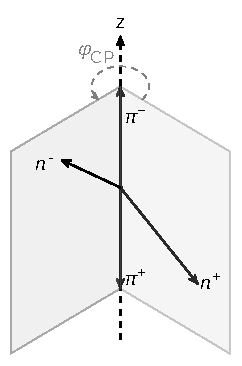
\includegraphics[width=0.4\textwidth]{Figures/Chapter7/Acoplanarity/Diagrams/IP-IP.pdf}
    \caption[Acoplanarity angle $\phi_{CP}$ reconstructed in the $\tauh\tauh \to \pi\pi$ category using the impact parameter method.]
    {Acoplanarity angle $\phi_{CP}$ reconstructed in the $\tauh\tauh \to \pi\pi$ category using the \ac{IP} method.}
    \label{Figure:Chapter7_IP_IP_Method}
\end{figure}

The method reconstructs each $\tau$ decay plane from the spatial momentum of the charged decay product ($\mathbf{q^\pm}$) together with its associated \ac{IP} vector ($\mathbf{n^\pm}$), as defined in Section~\ref{Section:Chapter4_Vertex_reconstruction}. These are expressed as four-vectors: the four-momentum of the charged particle $q^\pm$ and the impact-parameter four-vector $n^\pm = (0,\mathbf{n^\pm})$, both measured in the laboratory frame. The set of four-vectors is then boosted into the rest frame of the two charged particles, \ie the visible ditau \ac{ZMF} (denoted by $_\text{ZMF}$). In the \ac{ZMF}, the boosted \ac{IP} three-vector is normalised and decomposed into components parallel and transverse to the corresponding normalised three-momentum vector of the charged particle. From these, two key observables are defined: $\phi_{\text{ZMF}}$ and $O_{\text{ZMF}}$\footnote{The observable $O_{\text{ZMF}}$ resolves the twofold ambiguity in the angle between decay planes, which would otherwise be confined to the interval $[0,\pi]$. Its sign encodes the relative orientation (clockwise or anticlockwise) of the planes, thereby unfolding the acoplanarity angle to the full range $[0,2\pi]$ and retaining sensitivity to the CP phase of the $\PH\tau\tau$ coupling.}.
\begin{equation_pad}
    \phi_{\text{ZMF}} = \arccos(\hat{\mathbf{n}}_{\text{ZMF},\perp}^{+} \, \, \cdot \, \, \hat{\mathbf{n}}_{\text{ZMF},\perp}^{-})
\end{equation_pad}
\begin{equation_pad}
    O_{\text{ZMF}} = \hat{\mathbf{q}}^-_\text{ZMF} \, \, \cdot \, \,(\hat{\mathbf{n}}_{\text{ZMF},\perp}^{+} \, \, \times \, \, \hat{\mathbf{n}}_{\text{ZMF},\perp}^{-})
\end{equation_pad}

The acoplanarity angle is then defined over the full range $[0,2\pi]$ by:

\begin{equation_pad}
\phi_{CP} \;=\;
\begin{cases}
\phi_{\text{ZMF}} & O_{\text{ZMF}} \ge 0 \\
2\pi - \phi_{\text{ZMF}} & O_{\text{ZMF}} < 0
\end{cases}
\end{equation_pad}

The performance of the \ac{IP} method is illustrated by the reconstructed $\phi_{CP}$ distribution in the $\pi\pi$ category, shown in Fig.~\ref{Figure:CPDist_IPMethod_pipi}.

\begin{figure}[!htbp]
    \centering
    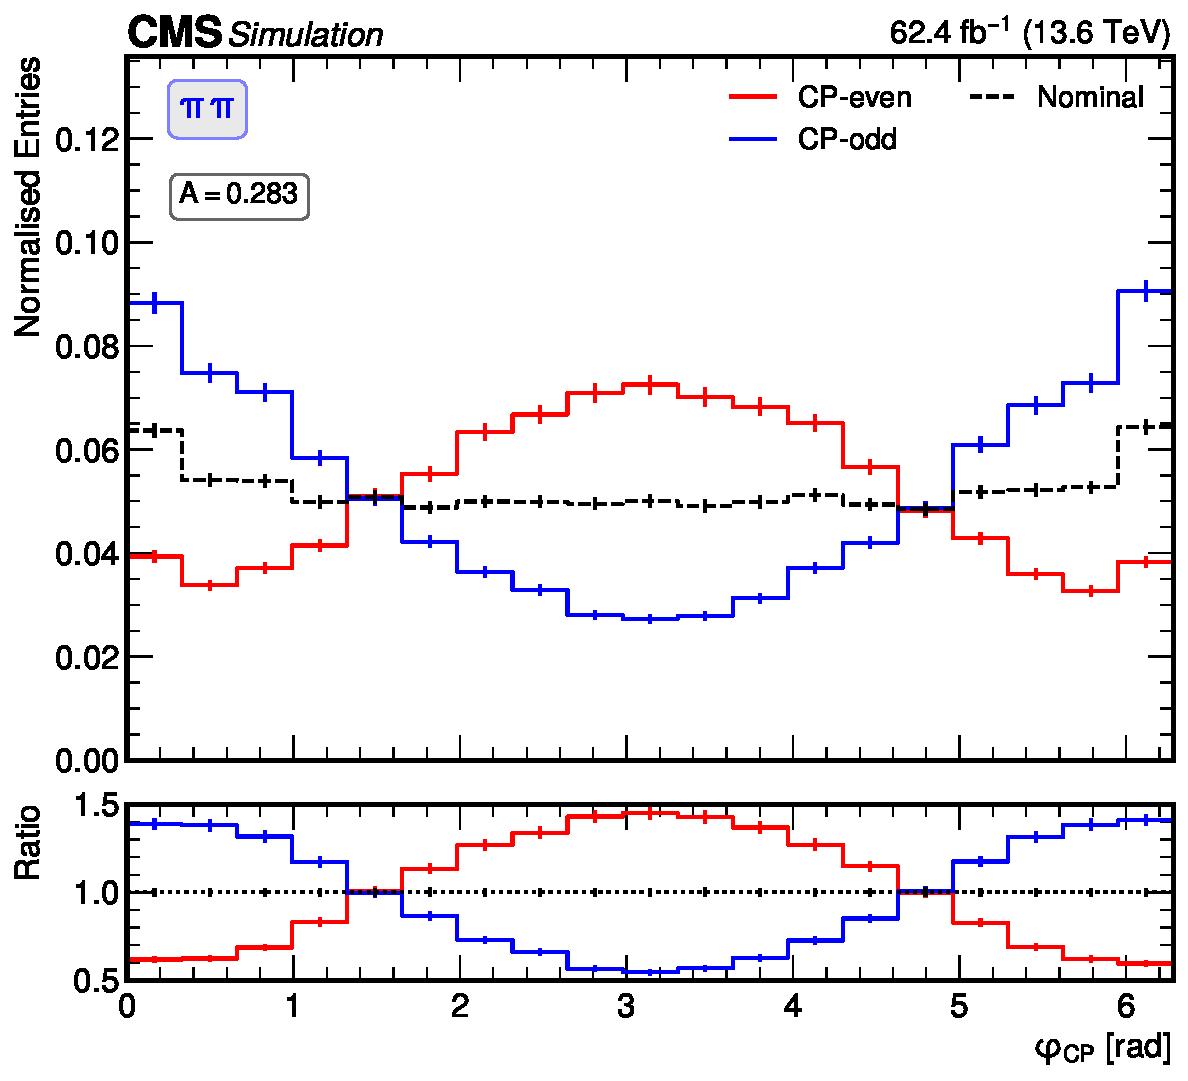
\includegraphics[width=0.6\textwidth]{Figures/Chapter7/Acoplanarity/With_IP/aco_pi_pi.pdf}
    \caption[Reconstructed $\phi_{CP}$ distribution in the $\tauh\tauh \to \pi\pi$ category using the impact parameter method.]
    {Reconstructed distribution of the acoplanarity angle $\phi_{CP}$ in the $\tauh\tauh \to \pi\pi$ category, obtained with the \ac{IP} method. The plots are obtained from the signal samples used in this analysis.}
    \label{Figure:CPDist_IPMethod_pipi}
\end{figure}

\subsection{Neutral-pion method}
\label{Section:NeutralPionMethod}

The \ac{NP} method, also referred to as the \textit{decay-plane method}, is designed for $\tau$ decays via the $\rho^\pm$ resonance, \ie $\tau^\pm \to \rho^\pm \nu_\tau$ with $\rho^\pm \to \pi^\pm \pi^0$. A schematic illustration of this method is shown in Fig.~\ref{Figure:Chapter7_NP_Method}. In this case, the $\tau$ decay plane is reconstructed from the momentum vectors of the charged pion ($\mathbf{q^\pm}$) and the neutral pion ($\mathbf{q^{0\pm}}$). Here, the neutral pion provides the secondary axis defining the plane, replacing the \ac{IP} vector used in the \ac{IP} method (Section~\ref{Section:Chapter7_IP_METHOD}).  

\begin{figure}[!htbp]
    \centering
    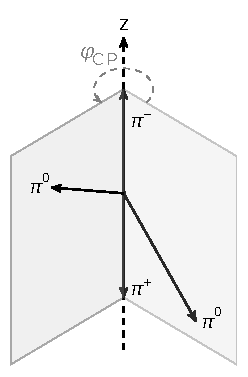
\includegraphics[width=0.4\textwidth]{Figures/Chapter7/Acoplanarity/Diagrams/NP-NP.pdf}
    \caption[Acoplanarity angle $\phi_{CP}$ reconstructed in the $\tauh\tauh \to \rho\rho$ category using the neutral-pion method.]
    {Acoplanarity angle $\phi_{CP}$ reconstructed in the $\tauh\tauh \to \rho\rho$ category using the \ac{NP} method.}
    \label{Figure:Chapter7_NP_Method}
\end{figure}

In analogy with the IP construction, the acoplanarity angle is first defined as,

\begin{equation_pad}
    \phi_{\text{ZMF}} = \arccos(\hat{\mathbf{q}}^{0+}_{\text{ZMF},\perp} \cdot \hat{\mathbf{q}}^{0-}_{\text{ZMF},\perp}),
\end{equation_pad}

where the transverse components of the neutral pion momenta are taken with respect to the associated charged-pion directions in the visible ditau \ac{ZMF}. To resolve the twofold ambiguity, a triple product observable is constructed as,

\begin{equation_pad}
    O_{\text{ZMF}} = \hat{\mathbf{q}}^-_{\text{ZMF}} \cdot (\hat{\mathbf{q}}^{0+}_{\text{ZMF},\perp} \times \hat{\mathbf{q}}^{0-}_{\text{ZMF},\perp}),
\end{equation_pad}

and the sign of $O_{\text{ZMF}}$ unfolds the angle to the full $[0,2\pi]$ range, thereby defining $\phi^\prime_{CP}$ as the signed acoplanarity angle:

\begin{equation_pad}
\phi^{\prime}_{CP} =
\begin{cases}
\phi_{\text{ZMF}}, & O_{\text{ZMF}} \ge 0 \\
2\pi - \phi_{\text{ZMF}}, & O_{\text{ZMF}} < 0
\end{cases}
\end{equation_pad}  

An additional refinement, specific to the $\rho$ channel, exploits the \textit{spin-analyser function},

\begin{equation_pad}
    y_\rho^\pm = \frac{E_{\pi^\pm} - E_{\pi^0}}{E_{\pi^\pm} + E_{\pi^0}},
\end{equation_pad}

where $E_{\pi^\pm}$ and $E_{\pi^0}$ are the energies of the charged and neutral pions in the laboratory frame. The product $y_\rho^+ y_\rho^-$ encodes the relative orientation of the spin-analyser vectors for the two $\tau$ decays and enhances the CP sensitivity. The final observable is thus defined as

\begin{equation_pad}
\phi_{CP} =
\begin{cases}
\phi^\prime_{CP}, & y_\rho^+ y_\rho^- \geq 0 \\
\phi^\prime_{CP} + \pi \; \,(\text{mod } 2\pi), & y_\rho^+ y_\rho^- < 0
\end{cases}
\end{equation_pad}

The performance of the \ac{NP} method is demonstrated in Fig.~\ref{Figure:CPDist_NPMethod}, which shows the reconstructed $\phi_{CP}$ distribution for the $\rho\rho$ category.

\begin{figure}[!htbp]
    \centering
    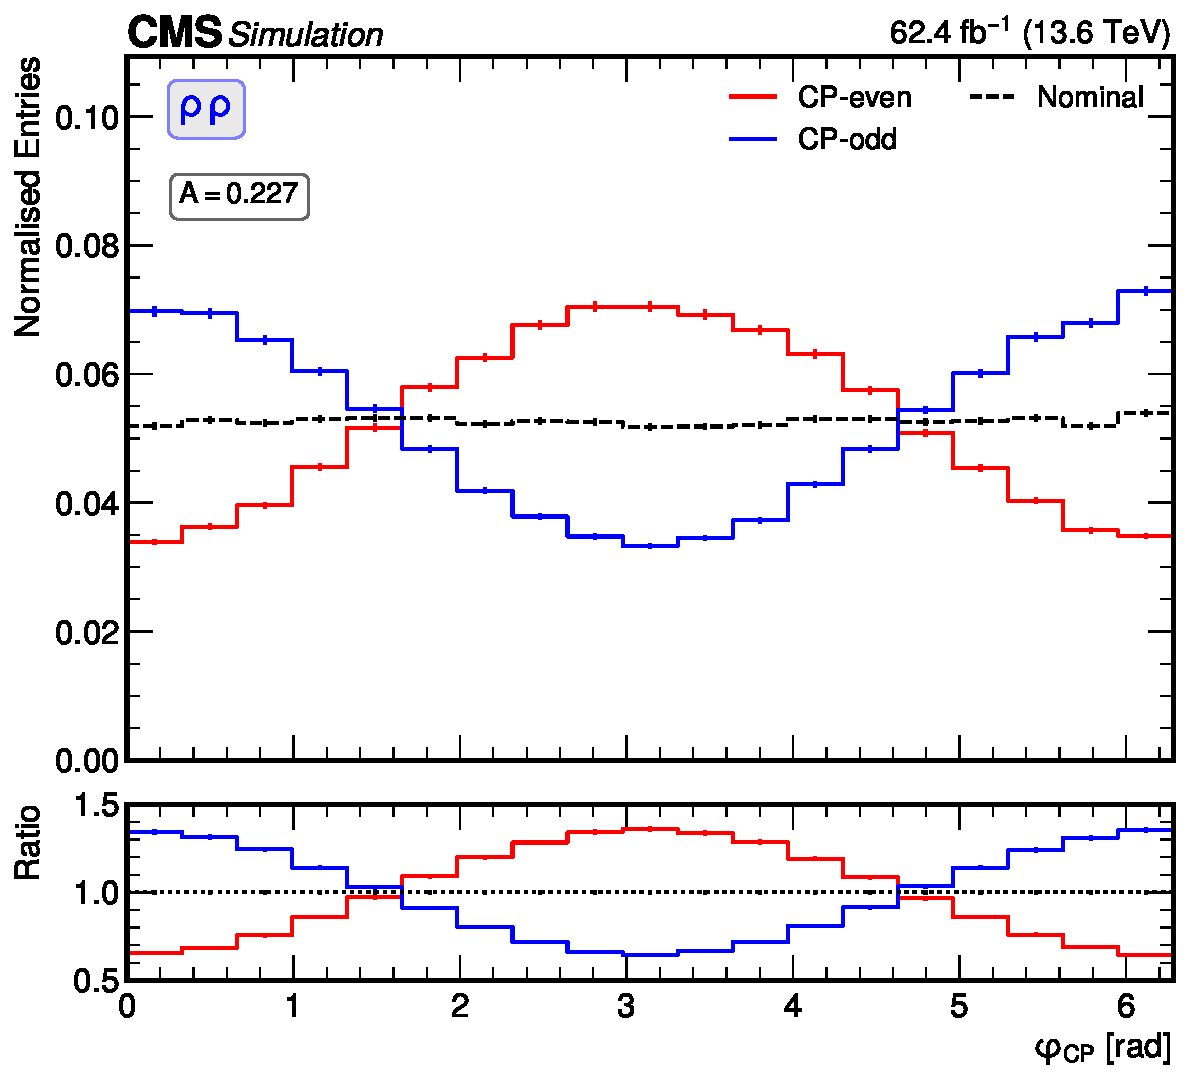
\includegraphics[width=0.6\textwidth]{Figures/Chapter7/Acoplanarity/With_IP/aco_rho_rho.pdf}
    \caption[Reconstructed $\phi_{CP}$ distribution in the $\tauh\tauh\to\rho\rho$ category using the neutral-pion method.]
    {Reconstructed distribution of the acoplanarity angle $\phi_{CP}$ in the $\tauh\tauh \to \rho\rho$ category, obtained with the \ac{NP} method from signal simulation.}
    \label{Figure:CPDist_NPMethod}
\end{figure}

\subsection{Polarimetric vector method in the $a_1^{3\mathrm{pr}}a_1^{3\mathrm{pr}}$ channel}
\label{Section:Chapter7_PV_Method}
The \ac{P.V.} method exploits the fact that, for certain $\tau$ \acp{DM}, the full kinematics of the $\tau$ lepton can be reconstructed with sufficient accuracy. This is the case when both $\tau$ leptons decay via the $a_1^\text{3pr}$ resonance, in which the \acp{SV} can be reconstructed from the three charged tracks of each decay. The $\tau$ lepton momentum direction is taken from the line connecting the \ac{PV} and \ac{SV}. Its magnitude is determined from the two-body decay kinematics $\tau \to a_1\nu_\tau$ under the assumptions of fixed $m_\tau$ and $m_{a_1}$ and a massless neutrino, as follows:

\begin{equation_pad}
|\vec{p}_\tau| = 
\frac{(m_{a_1}^2 + m_\tau^2)\,|\vec{p}_{a_1}| \cos\theta_{\mathrm{GJ}} \;\pm\; 
\sqrt{(m_{a_1}^2 + |\vec{p}_{a_1}|^2)\,\big[(m_{a_1}^2 - m_\tau^2)^2 - 4m_\tau^2 |\vec{p}_{a_1}|^2 \sin^2\theta_{\mathrm{GJ}}\big]}}
{2\,(m_{a_1}^2 + |\vec{p}_{a_1}|^2 \sin^2\theta_{\mathrm{GJ}})}.
\label{Equation:TauPTMag_PV}
\end{equation_pad}

Here $\theta_{\mathrm{GJ}}$ is the Gottfried--Jackson angle~\cite{Cherepanov:2018npf}, defined as the angle between the $\tau$ and $a_1$ momenta in the laboratory frame, and is constrained to lie within a physical maximum $\theta_{\mathrm{GJ}}^{\mathrm{max}}$. In practice, detector resolution effects may lead to $\theta_{\mathrm{GJ}} > \theta_{\mathrm{GJ}}^{\mathrm{max}}$, in which case $\theta_{\mathrm{GJ}}$ is set to $\theta_{\mathrm{GJ}}^{\mathrm{max}}$.  

Equation~\ref{Equation:TauPTMag_PV} admits two possible solutions for the magnitude of the $\tau$ lepton momentum. This ambiguity arises because, in the $\tau$ rest frame, the $a_1$ meson can be emitted either in the same direction as, or opposite to, the $\tau$ momentum in the laboratory frame. The case where the $a_1$ is emitted orthogonally corresponds to the unique solution in which the square root term vanishes. When applied to both $\tau$ decays in an event, this leads in general to up to four candidate solutions for the pair of $\tau$ momenta. The ambiguity is resolved by choosing the solution whose reconstructed ditau mass is closest to the nominal Higgs boson mass.

With the $\tau$ four-momenta determined, the \acp{PV} $\mathbf{h}_1$ and $\mathbf{h}_2$ are computed using the resonance model implemented in \TAUOLA~\cite{Jadach:1990mz,Jezabek:1991qp,Jadach:1993hs}, calibrated with experimental parameters from CLEO~\cite{CLEO:1999rzk}. To build a CP-sensitive observable, $\mathbf{k_{1,2}}$ vectors are defined as,

\begin{equation_pad}
\mathbf{\hat{k}}_{1,2} = \frac{\mathbf{\hat{h}}_{1,2} \times \mathbf{\hat{n}}_{1,2}}{|\mathbf{\hat{h}}_{1,2} \times \mathbf{\hat{n}}_{1,2}|},
\end{equation_pad}

where $\mathbf{\hat{n}}_{1,2}$ denote the unit vectors of the $\tau$ momenta in the Higgs rest frame. From these, the acoplanarity angle $\phi^*$ and the triple product observable $O^*$ are constructed as,  

\begin{equation_pad}
    \phi^* = \arccos(\mathbf{k}_1 \cdot \mathbf{k}_2)
\end{equation_pad}
\begin{equation_pad}
    O^* = - (\mathbf{\hat{h}}_1 \times \mathbf{\hat{h}}_2) \cdot \mathbf{\hat{n}}_1
\end{equation_pad}

with $^*$ denoting quantities in the Higgs rest frame. The final CP-sensitive observable is defined as,

\begin{equation_pad}
\phi_{CP} \;=\;
\begin{cases}
\phi^* & O^* \ge 0 \\
2\pi - \phi^* & O^* < 0
\end{cases}
\end{equation_pad}

An example of the $\phi_{CP}$ distribution reconstructed with the \ac{P.V.} method in the $a_1^{3\mathrm{pr}}a_1^{3\mathrm{pr}}$ category is shown in Fig.~\ref{Figure:CPDist_PVMethod}.

\begin{figure}[!htbp]
    \centering
    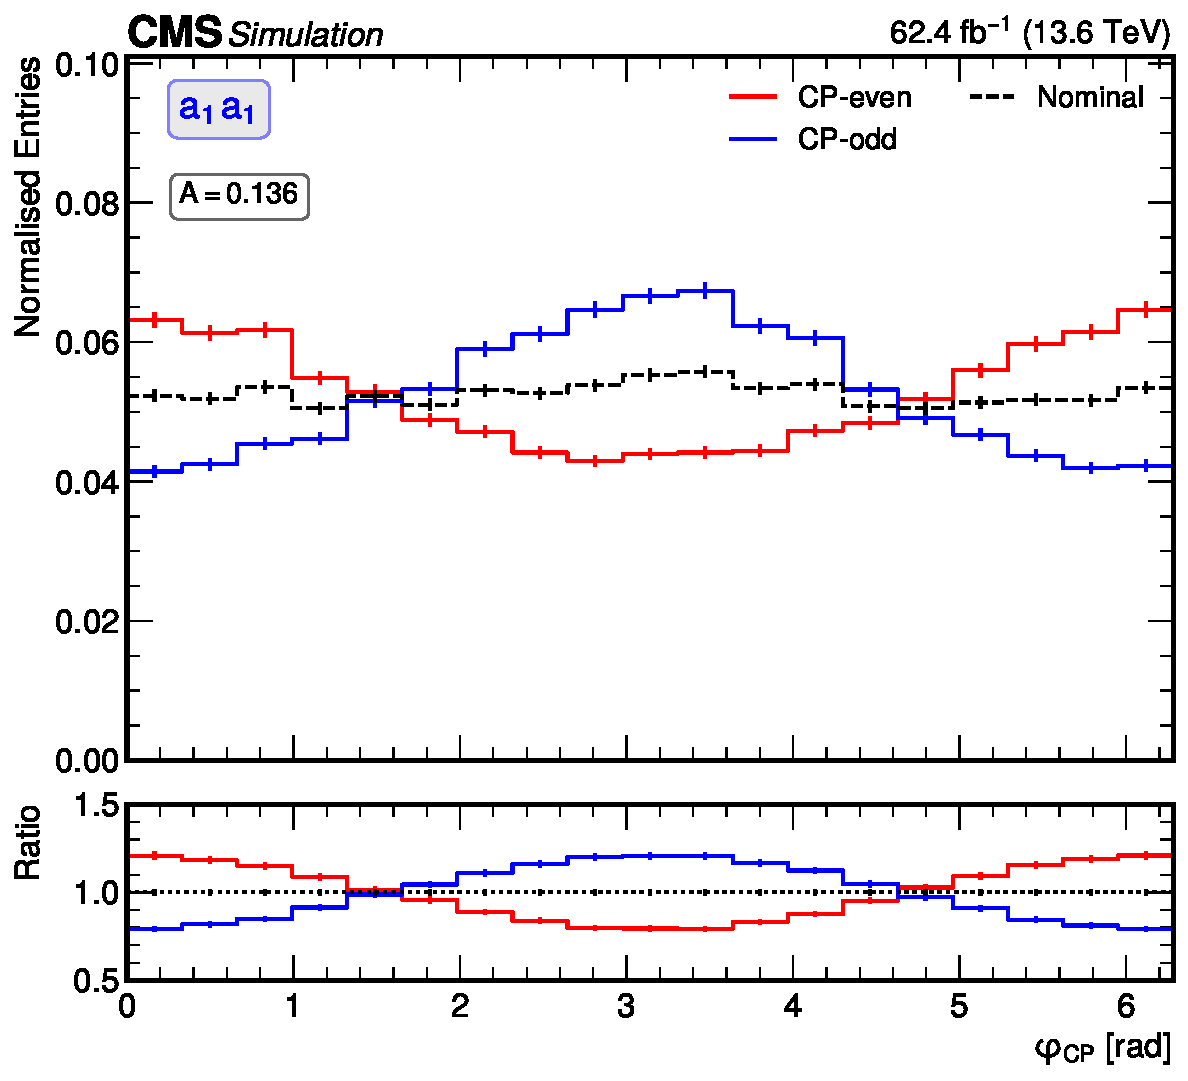
\includegraphics[width=0.6\textwidth]{Figures/Chapter7/Acoplanarity/With_IP/aco_a1_a1.pdf}
    \caption[Reconstructed $\phi_{CP}$ distribution in the $\tauh\tauh\to a_1^\text{3pr}a_1^\text{3pr}$ category using the \ac{P.V.} method.]
    {Reconstructed distribution of the acoplanarity angle $\phi_{CP}$ in the $\tauh\tauh \to a_1^\text{3pr}a_1^\text{3pr}$ category, obtained with the \ac{P.V.} method.}
    \label{Figure:CPDist_PVMethod}
\end{figure}

\subsection{Combined methods}
\label{Section:Chapter7_CombinedMethods}

The first combined method utilises both the \ac{IP} and \ac{NP} techniques, applied in channels where the two $\tau$ leptons decay through different modes. In particular, this strategy is relevant in the $\tauh\tauh \to \rho\pi$ category. In such cases, the decay plane of the $\tau_h\to\rho$ is reconstructed with the \ac{NP} method, while the other is reconstructed with the \ac{IP} method. The two planes are then combined in the visible ditau \ac{ZMF} to define $\phi_{CP}$. A schematic illustration of this method is shown in Fig.~\ref{Figure:Chapter7_IPNP_Method}.

\begin{figure}[!htbp]
    \centering
    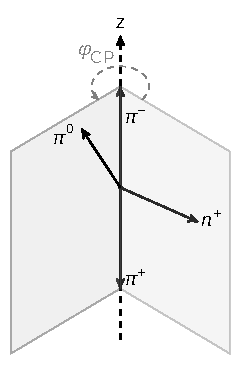
\includegraphics[width=0.4\textwidth]{Figures/Chapter7/Acoplanarity/Diagrams/IP-NP.pdf}
    \caption[Acoplanarity angle $\phi_{CP}$ reconstructed in the $\tauh\tauh \to \rho\pi$ category using the combined neutral-pion \& impact parameter method.]
    {Acoplanarity angle $\phi_{CP}$ reconstructed in the $\tauh\tauh \to \rho\pi$ category using the combined \ac{NP}-\ac{IP} method.}
    \label{Figure:Chapter7_IPNP_Method}
\end{figure}

A subtlety arises because the \ac{NP} method introduces a sign ambiguity, which requires redefining $\phi_{CP}$ as

\begin{equation_pad}
\phi_{CP} =
\begin{cases}
\phi^\prime_{CP} & y_\rho \geq 0 \\
\phi^\prime_{CP} + \pi \; \,(\text{mod } 2\pi) & y_\rho < 0
\end{cases}
\end{equation_pad}

The resulting $\phi_{CP}$ distribution obtained with the \ac{IP}-\ac{NP} combined method is shown in Fig.~\ref{Figure:CPDist_Combined_IP_NP}, illustrating the complementarity of the different approaches across categories.

\begin{figure}[!htbp]
    \centering
    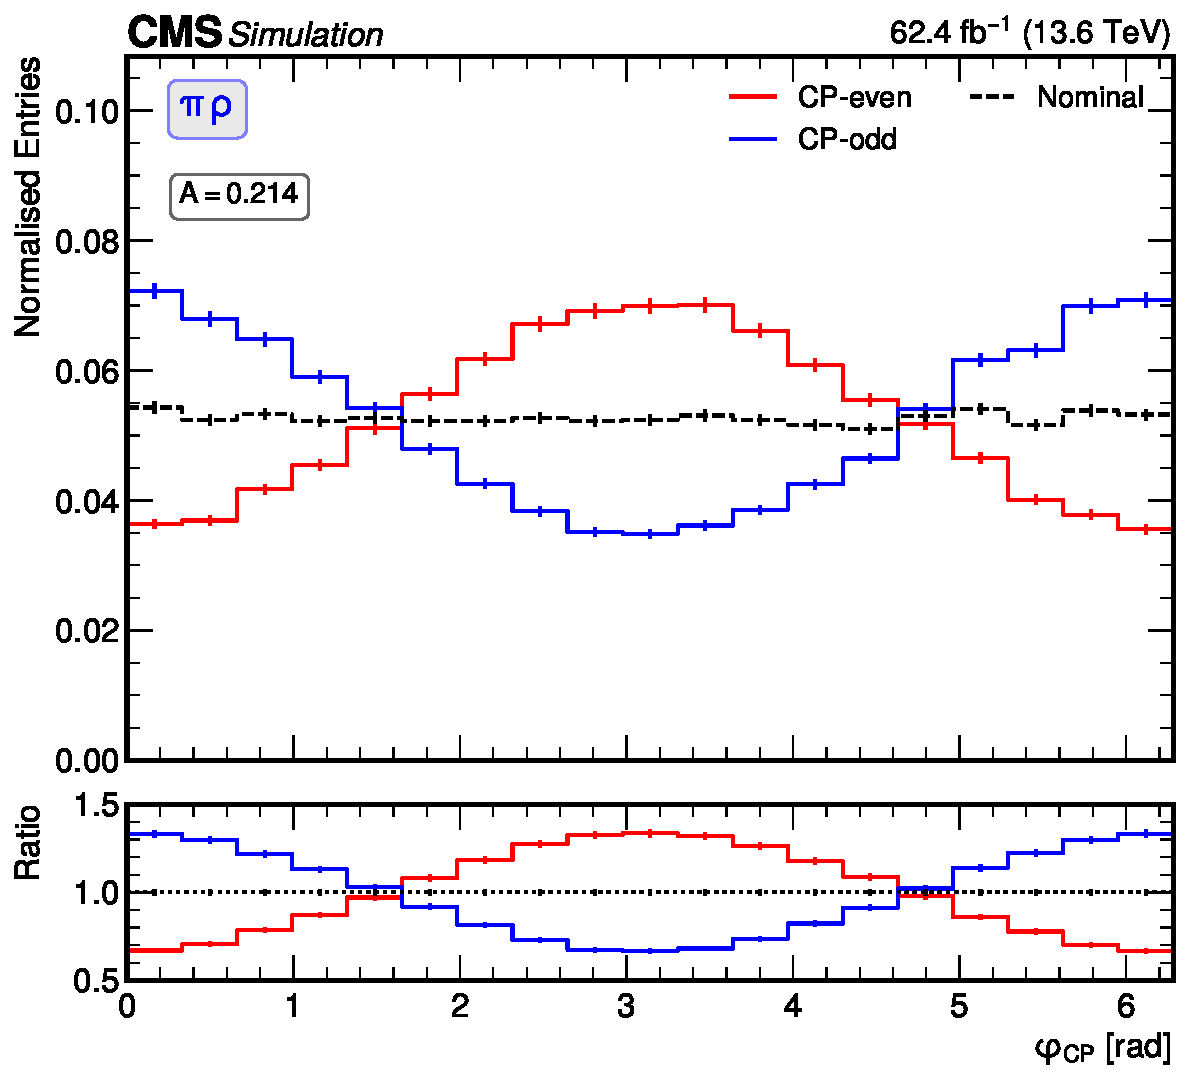
\includegraphics[width=0.5\textwidth]{Figures/Chapter7/Acoplanarity/With_IP/aco_pi_rho.pdf}
    \caption[Reconstructed $\phi_{CP}$ distribution in the $\tau_h\tau_h\to\pi\rho$ category using the IP-NP combined method.]
    {Reconstructed distribution of the acoplanarity angle $\phi_{CP}$ in the $\tauh\tauh \to \pi\rho$ final state, obtained with the \ac{IP}-\ac{NP} combined method. The plots are obtained from the signal samples used in this analysis.}
    \label{Figure:CPDist_Combined_IP_NP}
\end{figure}

The second combined method applies to events where one $\tau$ lepton decays via the $a_1^\text{3pr}$ mode and the other through a single-prong decay ($\pi$ or $\rho$), with the latter reconstructed using the \ac{IP} or \ac{NP} method. The plane associated with the $a_1^\text{3pr}$ leg is reconstructed analogously to the pure $a_1^\text{3pr}$$a_1^\text{3pr}$ \ac{P.V.} method, where the $\tau$ flight direction is approximated by the line between the \ac{SV} and the \ac{PV}. The $\tau$ momentum magnitude is obtained from a kinematic fit. In this analysis, the \textsc{FastMTT} algorithm~\cite{Bianchini:2014vza} is employed, constraining the ditau invariant mass to $m_H$. The resulting four-vector is constructed assuming the nominal $\tau$ mass and truncated to enforce the physical maximum of the Gottfried-Jackson angle. The \ac{P.V.} of the $a_1^\text{3pr}$ leg is then calculated as described in Section~\ref{Section:Chapter7_PV_Method}.

The acoplanarity angle $\phi_{CP}$ is reconstructed by combining the \ac{P.V.} on the $a_1^{3\text{pr}}$ leg with the decay plane from the other $\tau$ leg (either \ac{IP}- or \ac{NP}-based). The same $y_\rho$ sign correction introduced for the first combined method is applied here to resolve the sign ambiguity when the \ac{NP} method is used. The reconstructed $\phi_{CP}$ distributions obtained with the combined \ac{IP}/\ac{NP}--\ac{P.V.} method are shown in Fig.~\ref{Figure:CPDist_Combined_IPNP_PV}.

\begin{figure}[!htbp]
        \centering
        % First row
        \begin{subfigure}[b]{0.49\textwidth}
            \centering
            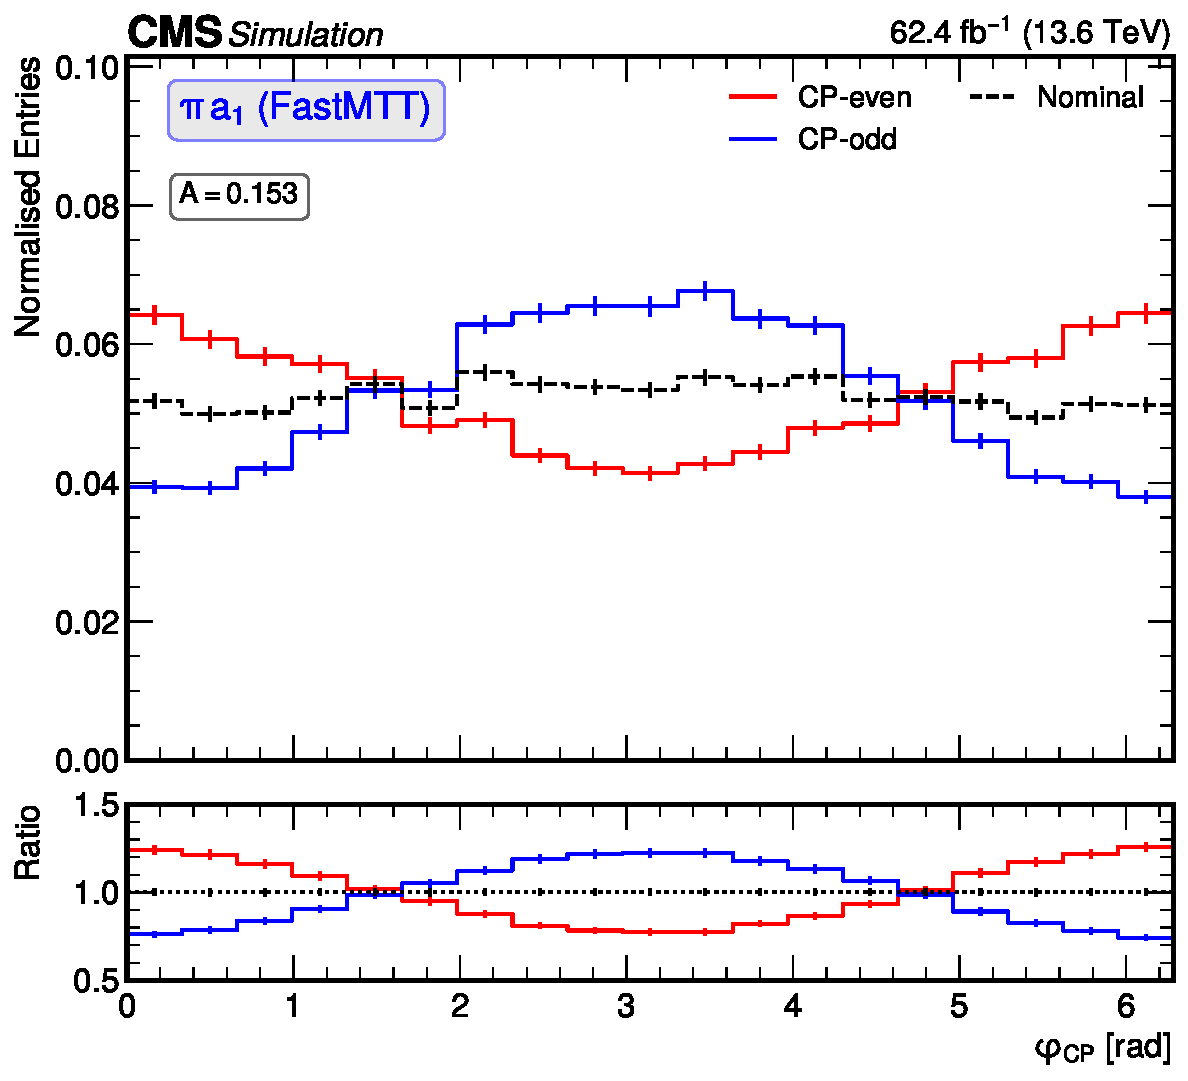
\includegraphics[width=\textwidth]{Figures/Chapter7/Acoplanarity/With_IP/aco_pi_a1_FASTMTT_MassConstraint.pdf}
            \caption{}
        \end{subfigure}
        \begin{subfigure}[b]{0.49\textwidth}
            \centering
            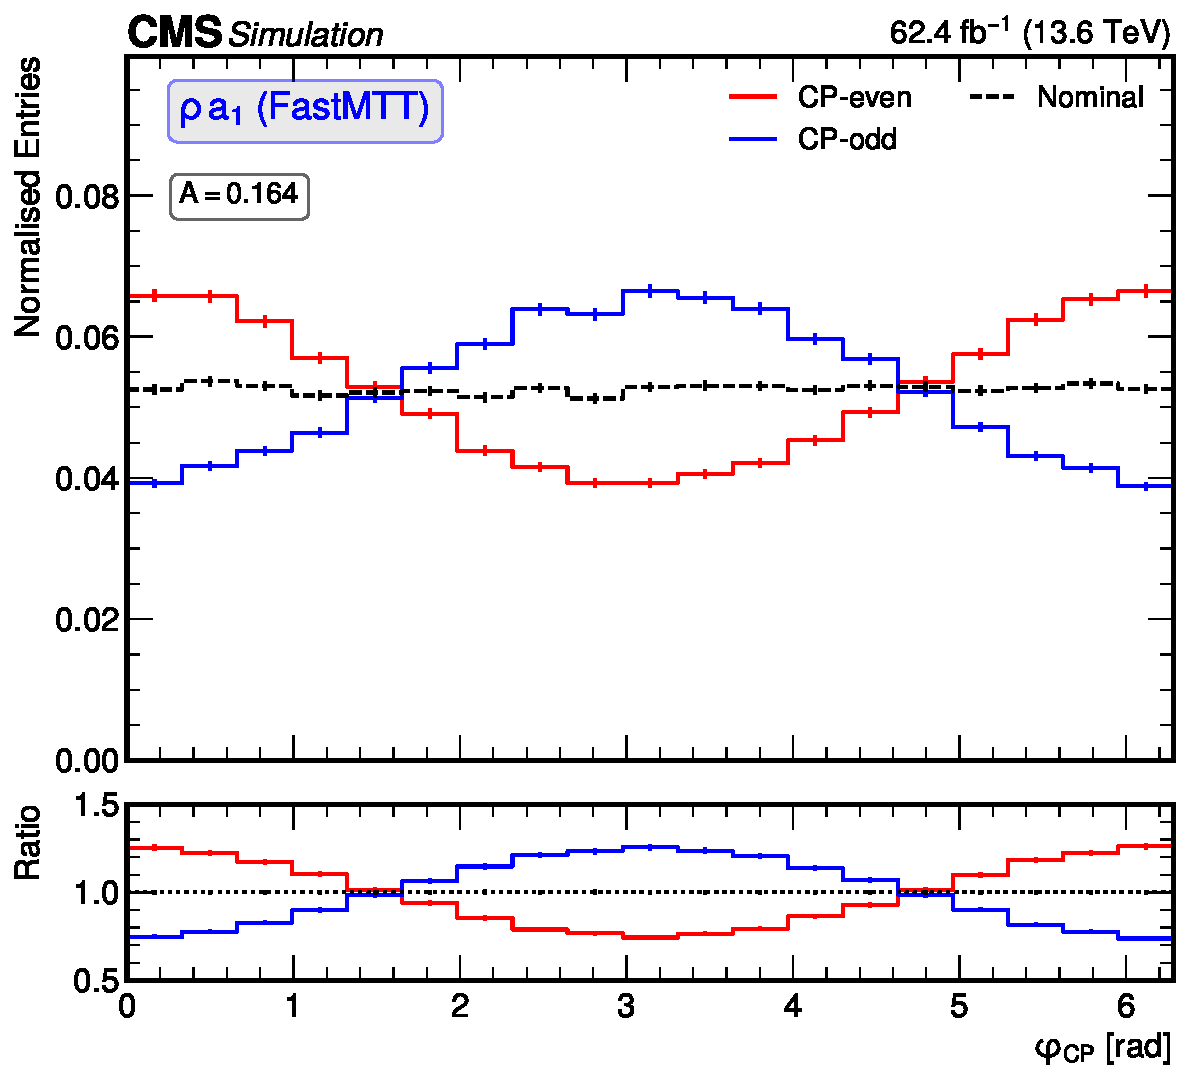
\includegraphics[width=\textwidth]{Figures/Chapter7/Acoplanarity/With_IP/aco_rho_a1_FASTMTT_MassConstraint.pdf}
            \caption{}
        \end{subfigure}
    \caption[Reconstructed $\phi_{CP}$ distributions with the combined IP/NP--PV method.]
    {Reconstructed distributions of the acoplanarity angle $\phi_{CP}$ in categories where one $\tau$ decays via the $a_1^{3\mathrm{pr}}$ resonance and the other through a single-prong decay; \textbf{(a)} $\pi$, \textbf{(b)} $\rho$.}
    \label{Figure:CPDist_Combined_IPNP_PV}
\end{figure}

\subsection{Summary of reconstruction strategy}
\label{Section:Chapter7_MethodSummary}

For each $\tauh\tauh$ category, the acoplanarity angle $\phi_{CP}$ is reconstructed using the method that provides the highest CP sensitivity. The mapping adopted in this analysis is summarised in Table~\ref{Table:Chapter7_ReconstructionMethodSummary}.


\begin{table}[!htbp]
\centering
\renewcommand{\arraystretch}{1.5} % Increase row height
\setlength{\tabcolsep}{10pt} % Increase column width
\arrayrulecolor{black} % Ensure outer border is black
\begin{tabular}{ccc}
\hline
Category & Method Leg$_1$ & Method Leg$_2$\\
\hline
$\pi\pi$       & \ac{IP} & \ac{IP} \\
\arrayrulecolor{lightgray} \hline
$\pi\rho$       & \ac{IP} & \ac{NP} \\
\arrayrulecolor{lightgray} \hline
$\pi a_1^\text{1pr}$       & \ac{IP} & \ac{NP} \\
\arrayrulecolor{lightgray} \hline
$\pi a_1^\text{3pr}$       & \ac{IP} & \ac{P.V.}$^*$ \\
\arrayrulecolor{lightgray} \hline
$\rho\rho$       & \ac{NP} & \ac{NP} \\
\arrayrulecolor{lightgray} \hline
$\rho a_1^\text{1pr}$       & \ac{NP} & \ac{NP} \\
\arrayrulecolor{lightgray} \hline
$\rho a_1^\text{3pr}$       & \ac{IP} & \ac{P.V.}$^*$ \\
\arrayrulecolor{lightgray} \hline
$a_1^\text{1pr} a_1^\text{3pr}$       & \ac{NP} & \ac{P.V.}$^*$ \\
\arrayrulecolor{lightgray} \hline
$a_1^\text{3pr} a_1^\text{3pr}$       & \ac{P.V.} & \ac{P.V.} \\
\arrayrulecolor{black} \hline
\end{tabular}
\caption[Summary of reconstruction methods per $\tauh\tauh$ category.]
{Summary of the reconstruction strategy adopted for each $\tauh\tauh$ category in this analysis. The second column indicates the method applied to the first $\tau$ leg, while the third column indicates the method applied to the second $\tau$ leg. An asterisk ($^*$) marks cases where the reconstruction strategy differs from that used in the Run 2 analysis of Ref.~\cite{HiggsCP_CMS_2021}.}
\label{Table:Chapter7_ReconstructionMethodSummary}
\end{table}

As summarised in Table~\ref{Table:Chapter7_ReconstructionMethodSummary}, for categories involving one $a_1^{3\mathrm{pr}}$ resonance (\ie $X$–$a_1^{3\mathrm{pr}}$), the reconstruction strategy differs from that used in the earlier Run 2 analysis~\cite{HiggsCP_CMS_2021}. In the previous approach, such cases were reconstructed with a modified version of the \ac{NP} method. In the present analysis, this strategy has been superseded by the use of the \ac{P.V.} method, as described in Section~\ref{Section:Chapter7_CombinedMethods}. A direct comparison between the two strategies for the $X$–$a_1^{3\mathrm{pr}}$ channels is provided in Fig.~\ref{Figure:Chapter7_X-a1-Improvement}, using Run 3 signal simulation. This setup ensures that the observed differences reflect only the gain from the updated reconstruction method itself, disentangled from other improvements to the analysis chain summarised in Section~\ref{Section:Chapter7_Introduction}.

\begin{figure}[!htbp]
        \centering
        % First row
        \begin{subfigure}[b]{0.49\textwidth}
            \centering
            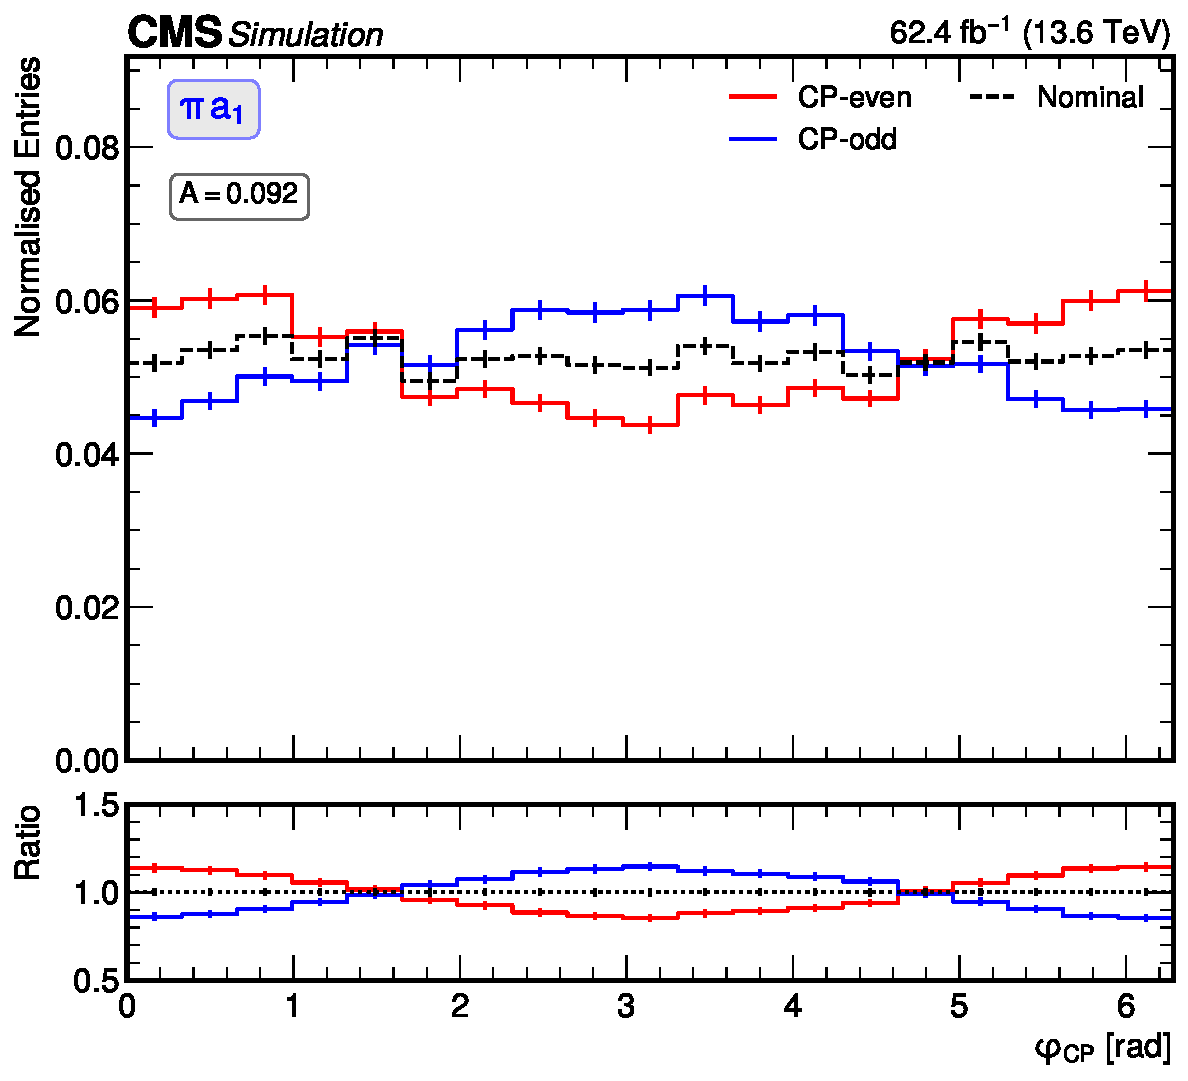
\includegraphics[width=\textwidth]{Figures/Chapter7/Acoplanarity/With_IP/aco_pi_a1.pdf}
            \caption{}
        \end{subfigure}
        \begin{subfigure}[b]{0.49\textwidth}
            \centering
            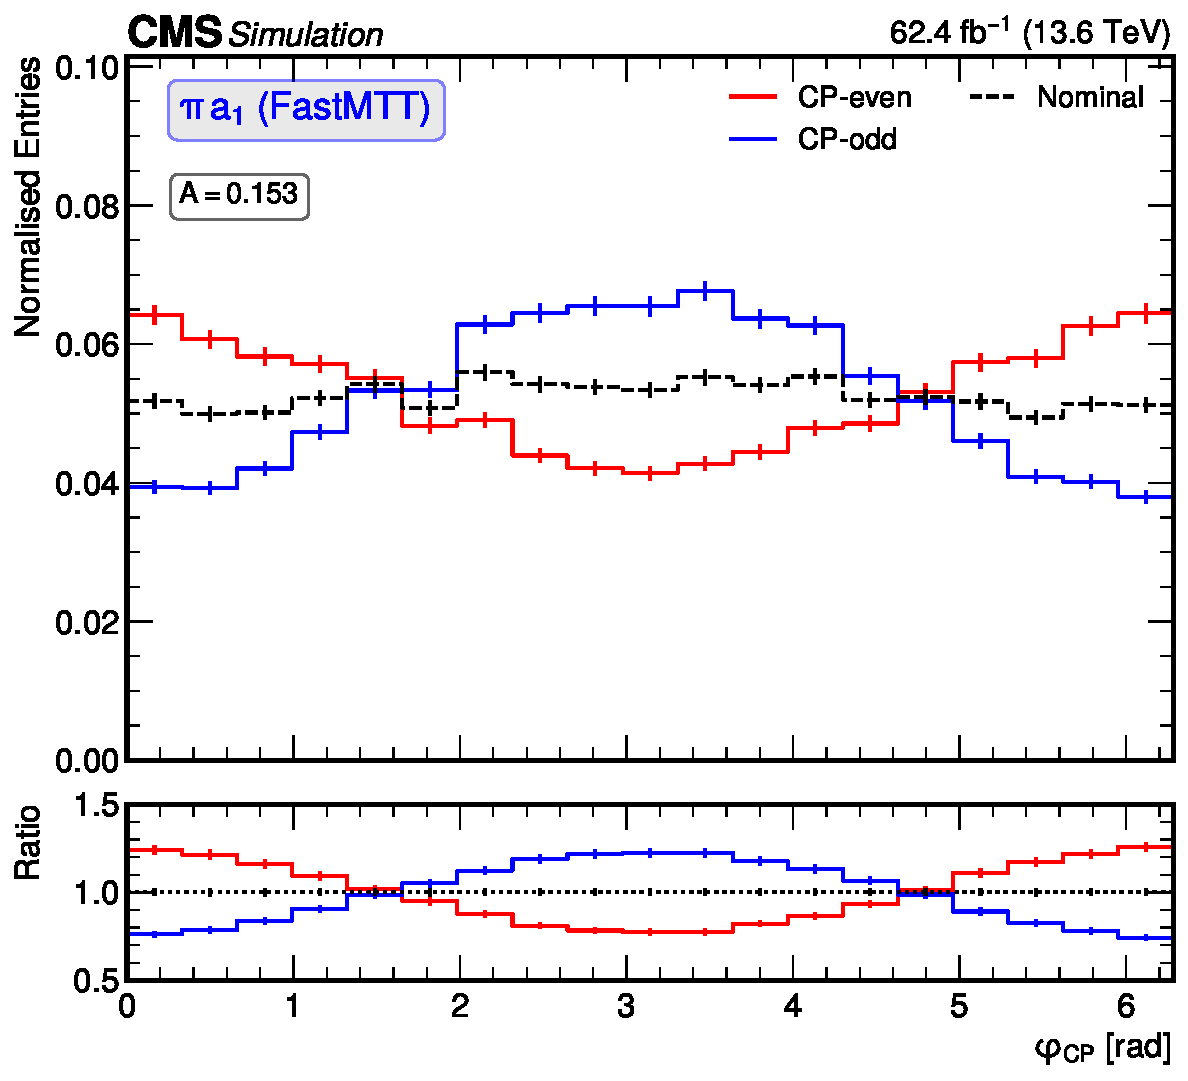
\includegraphics[width=\textwidth]{Figures/Chapter7/Acoplanarity/With_IP/aco_pi_a1_FASTMTT_MassConstraint.pdf}
            \caption{}
        \end{subfigure}
        \begin{subfigure}[b]{0.49\textwidth}
            \centering
            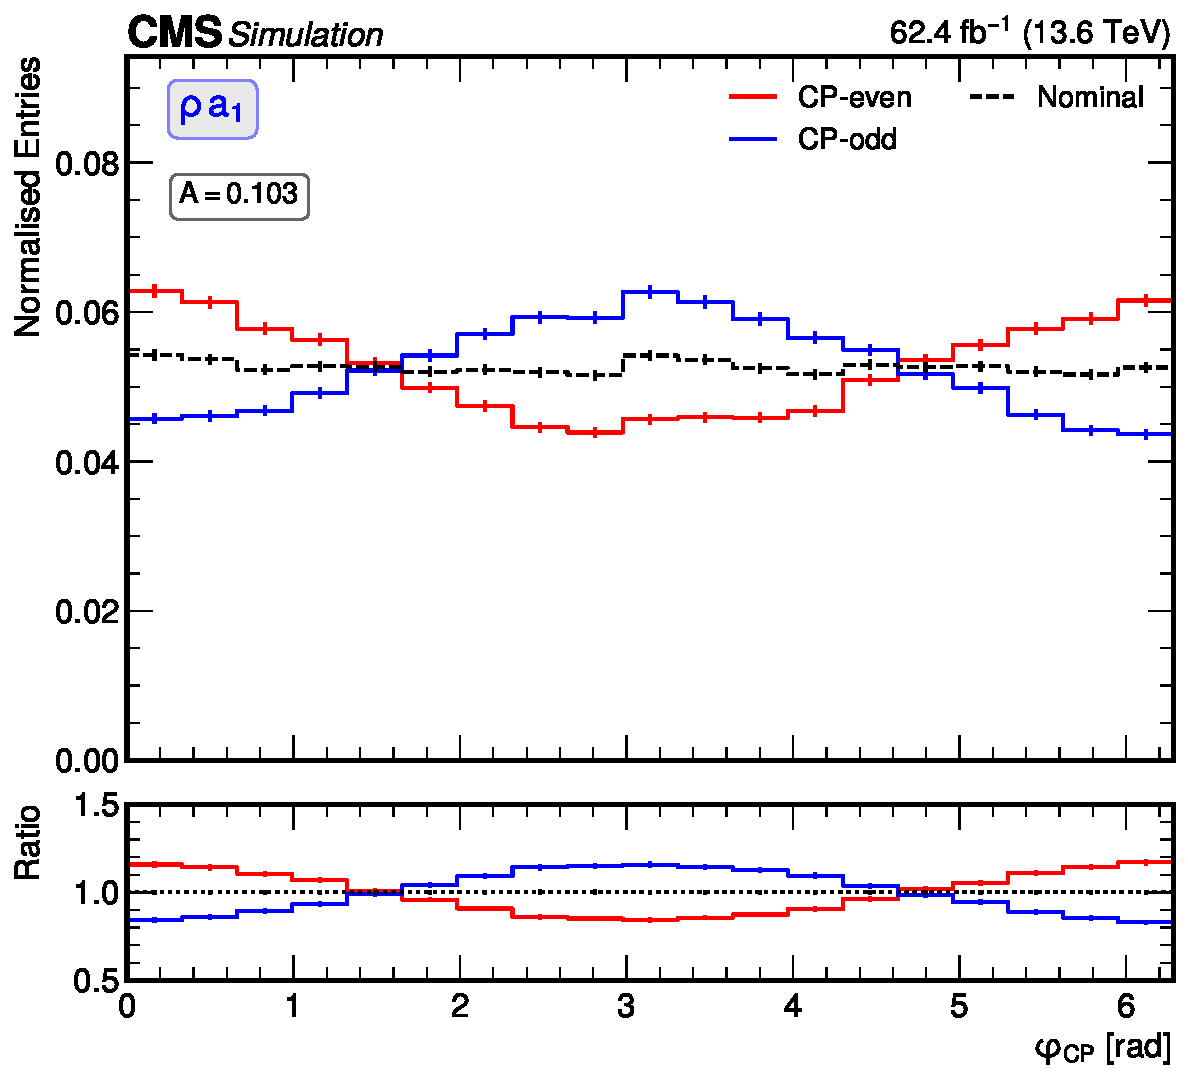
\includegraphics[width=\textwidth]{Figures/Chapter7/Acoplanarity/With_IP/aco_rho_a1.pdf}
            \caption{}
        \end{subfigure}
        \begin{subfigure}[b]{0.49\textwidth}
            \centering
            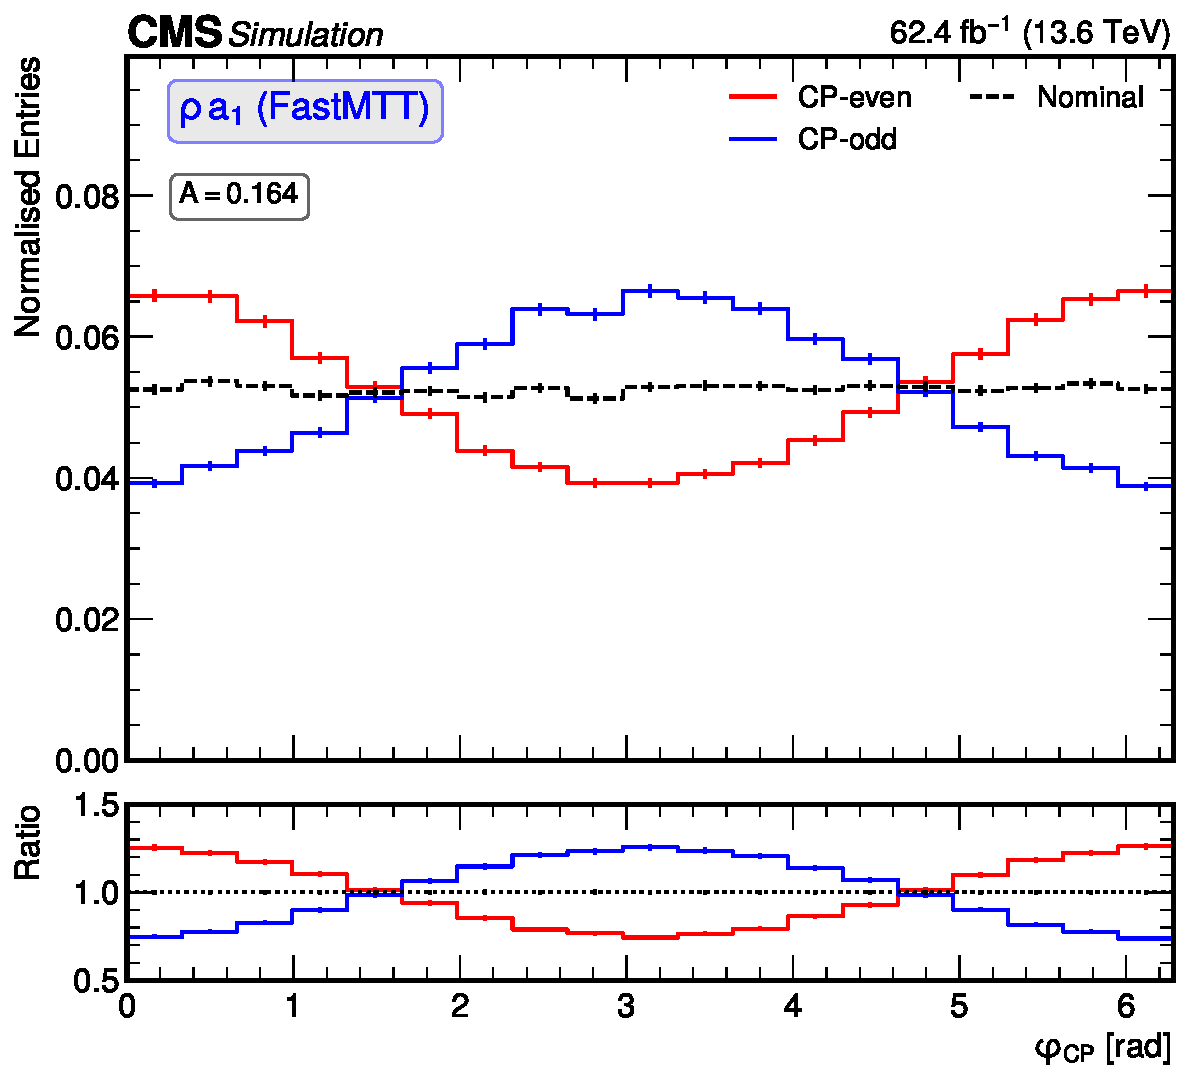
\includegraphics[width=\textwidth]{Figures/Chapter7/Acoplanarity/With_IP/aco_rho_a1_FASTMTT_MassConstraint.pdf}
            \caption{}
        \end{subfigure}
    \caption[Comparison of reconstruction strategies for $X$–$a_1^{3\mathrm{pr}}$ categories.]
    {Reconstructed $\phi_{CP}$ distributions in $X$–$a_1^{3\mathrm{pr}}$ categories. \textbf{(a,c)} show the Run 2 strategy using a modified \ac{NP} method for the $a_1$ leg, while \textbf{(b,d)} show the updated Run 3 strategy employing the \ac{P.V.} method. The comparison isolates the improvement from the new reconstruction approach.}
    \label{Figure:Chapter7_X-a1-Improvement}
\end{figure}

\section{Event selection strategy}
\label{Section:Chapter7_EventSelectionStrategy}

This analysis targets $\PH \to \tau\tau$ decays in the fully hadronic channel ($\tauh\tauh$), which accounts for the largest branching fraction among all ditau topologies ($\sim$42\%). The categories considered are those listed in Table~\ref{Table:Chapter7_ReconstructionMethodSummary}. In this section, the trigger requirements, offline object selections, and event-level selections are described.

\subsection{Triggering}
Events are selected online using two complementary triggers: a dedicated double-$\tau_h$ trigger and a double-$\tau_h$+jet trigger. The corresponding online $p_\text{T}$ thresholds are summarised in Table~\ref{Table:Chapter7_Triggers_TauhTauh}.

\begin{table}[!htbp]
\centering
\renewcommand{\arraystretch}{1.5}
\setlength{\tabcolsep}{12pt} % Increase column width
\begin{tabular}{|c|ccc|}
\hline
\multirow{3}{*}{Trigger}
  & \multicolumn{3}{c|}{$p_\text{T}$ (GeV)} \\ \cline{2-4}
  & \multicolumn{3}{c|}{2022--2023} \\ \cline{2-4}
  & Obj$_1$ & Obj$_2$ & Jet$_1$ \\ \hline\hline
Double-Tau ($\tau\tau$) & 35 & 35 & -- \\
\arrayrulecolor{lightgray}\hline
Double-Tau + jet ($\tau\tau$ + jet) & 30 & 30 & 60 \\
\arrayrulecolor{black}\hline
\end{tabular}
\caption{Table of the minimum online $p_\text{T}$ thresholds for the triggers used in the analysis.}
\label{Table:Chapter7_Triggers_TauhTauh}
\end{table}

The double-$\tau_h$ trigger provides the baseline selection, while the additional double-$\tau_h$+jet path extends acceptance to events with lower-$p_\text{T}$ $\tau_h$ candidates and enhances sensitivity in jet-rich topologies such as \ac{VBF}. Although the two triggers could be used in an orthogonal manner, the analysis instead employs their logical OR. This increases the complexity of efficiency determination, as overlaps must be handled carefully, but ensures maximal signal acceptance and prevents losses in the transition region between the two triggers. 

\subsection{Offline object and event-level selections}
\label{Section:Chapter7_OfflineSelections}
The offline object selections closely follow those employed in the four-tau analysis described in Section~\ref{Section:Chapter6_ObjectSelection}, and are summarised in Table~\ref{Table:Chapter7_Tauh_SelectionSummary}. To maintain consistency between trigger and offline definitions, selected $\tau_h$ candidates are required to match the corresponding trigger objects within a cone of $\Delta R < 0.5$, with offline $p_\text{T}$ thresholds set 5\GeV above the online thresholds. At the event level, at least two $\tau_h$ candidates are required, with the leading pair chosen to form the $\tauh\tauh$ system. The pair must carry opposite charge and be separated by $\Delta R > 0.5$. Events containing isolated electrons or muons are vetoed ($\mathcal{N}_e = 0$, $\mathcal{N}_\mu = 0$) to ensure orthogonality with leptonic channels. 

{
\setlength{\arrayrulewidth}{1pt}

\begin{table}[!htbp]
\centering
\caption[Summary of baseline selection criteria for $\tau_h$ candidates in the $\tau_h\tau_h$ channel.]{
Summary of baseline selection criteria applied to hadronically decaying tau candidates in the $\tau_h\tau_h$ final state. Trigger-matched $p_\text{T}$ thresholds are defined relative to the online values of the double-$\tau_h$ trigger.}
\label{Table:Chapter7_Tauh_SelectionSummary}

\renewcommand{\arraystretch}{1.5}
\setlength{\tabcolsep}{12pt}
\arrayrulecolor{black}

\begin{tabular}{lc}
\hline
Criteria & Hadronic Tau ($\tau_h$) \\
\hline
$p_\text{T}$ (baseline) &  $> 35 \GeV$\\
\arrayrulecolor{lightgray} \hline

$p_\text{T}^{\text{Trigger}}$ & $ > \text{Table~\ref{Table:Chapter7_Triggers_TauhTauh}} + [5\GeV]$ \\
\arrayrulecolor{lightgray} \hline

$|\eta|$ & $< 2.1$ \\
\arrayrulecolor{lightgray} \hline

$|d_z|$ & $< 0.2\unit{cm}$ (see Chapter~\ref{Section:Chapter4}) \\
\arrayrulecolor{lightgray} \hline

Identification 
& \makecell{
\normalfont\footnotesize$D_{\text{jet}} \geq$ VTight\hyperlink{Alternative-FFcut_CP}{$^1$} \\
\normalfont\footnotesize$D_{e} \geq$ VVLoose \\
\normalfont\footnotesize$D_{\mu} \geq$ Tight
} \\ 
\arrayrulecolor{black} \hline
\end{tabular}
\vspace{0.5em}
\begin{minipage}{0.95\linewidth}
\raggedright
\footnotesize
\hypertarget{Alternative-FFcut_CP}{}$^{1}$\,The VTight \ac{WP} is referred to as the \texttt{Nominal} tau identification in the fake factor method (see Section~\ref{Section:Chapter7_FF}). An \texttt{Alternative} selection, defined as $D_{\text{jet}} >$ Loose, is used to construct control regions.

\end{minipage}
\end{table}
}

As discussed in Section~\ref{Section:Chapter7_PhiCP_Reconstruction}, the sensitivity of this analysis depends critically on the accurate classification of the $\tau$ \acp{DM}. In the previous iteration of this analysis, a dedicated \ac{MVA} was developed to improve upon the performance of the \ac{HPS} \ac{DM} classification (see Fig.~\ref{Figure:Chapter4_HPS_ConfusionMatrix}). In Run 3, this was superseded by \textsc{ParticleNet}~\cite{Qu:2019gqs}, which provides substantially improved classification performance and is therefore adopted throughout this analysis.  

In addition to the baseline selections, further refinements are introduced to enhance CP sensitivity in specific \acp{DM}. In modes relying on the \ac{IP} method, events with poorly measured \acp{IP} yield reduced discriminating power. To mitigate this, a requirement is imposed on the transverse \ac{IP} significance, IP$_\text{sig}$. This preferentially selects events where the \ac{IP}-based reconstruction is most effective. Similarly, in channels reconstructed with the \ac{NP} method, events with large values of $|y_\rho^+ y_\rho^-|$ provide stronger CP sensitivity\footnote{Here $y_\rho^\pm$ act as spin-analyser functions: values close to $\pm 1$ correspond to kinematic configurations where the $\tau$ spin information is maximally transferred to the visible $\pi^\pm\pi^0$ system.}. Hence, $|y_\rho|$ is also exploited to preferentially select such events. The refined selections used for each \ac{DM} are summarised in Table~\ref{Table:Chapter7_RefinedSelections_perDM}.  

\begin{table}[!htbp]
\centering
\renewcommand{\arraystretch}{1.5}
\setlength{\tabcolsep}{12pt}
\arrayrulecolor{black}

\begin{tabular}{ccc}
\hline
Decay mode & $\text{IP}_\text{sig}$ & $|y_\rho|$ \\
\hline
$\pi$ &  $> 1.25$ & -- \\
\arrayrulecolor{lightgray} \hline
$\rho$ &  -- & $> 0.2$ \\
\arrayrulecolor{lightgray} \hline
$a_1^\text{1pr}$ &  -- & $> 0.2$ \\
\arrayrulecolor{lightgray} \hline
$a_1^\text{3pr}$ &  -- & -- \\
\arrayrulecolor{black} \hline
\end{tabular}
\caption[Refined selection criteria per $\tau$ decay mode in the $\tauh\tauh$ channel.]{
Refined selection criteria per $\tau$ \ac{DM} in the $\tauh\tauh$ channel. The optimisation of these thresholds is described in Section~\ref{Section:Chapter7_OptimisingSelectionCriteria}.}
\label{Table:Chapter7_RefinedSelections_perDM}
\end{table}

\section{Object and event corrections}

This section summarises the object- and event-level corrections applied to simulation in this analysis. A subset of these follow directly from the procedures described for the four-tau analysis in Section~\ref{Section:Chapter6_Corrections}. The following corrections are derived and applied in the same way as in that analysis:

\begin{itemize}
    \item Pileup reweighting (Section~\ref{Section:Chapter6_PU})
    \item Hadronic tau misidentification rates (Section~\ref{Section:Chapter6_Lepton_MisID_SF})
\end{itemize}

However, not all corrections from Section~\ref{Section:Chapter6_Corrections} are transferable. Certain elements must be re-derived or adapted to account for the selections specific to this analysis. In particular, the hadronic tau identification, energy scale, and trigger efficiencies were re-derived. This was required because ParticleNet is used for \ac{DM} classification (instead of the \ac{HPS} algorithm), together with the optimised \ac{DM}-dependent selections summarised in Table~\ref{Table:Chapter7_RefinedSelections_perDM}. Despite these changes, the procedures for deriving the corrections remain unchanged from those described in Sections~\ref{Section:Chapter6_Tau_ID_ES}-\ref{Section:Chapter6_HadronicTauTrigger_Efficiencies}. The only distinction is that, in this analysis, the corrections are determined in bins of ParticleNet \ac{DM} and derived for $\tauh$ candidates passing the optimised \ac{DM}-dependent selections.

The remaining corrections that differ from the four-tau analysis are detailed in the following subsections.

\subsection{\texorpdfstring{$\PZ \, \, p_\text{T}$-mass reweighting}{Z pT-mass reweighting}}

\ac{DY} events generated at \ac{NLO} with $\MADGRAPH$ do not accurately describe the kinematic regime in which the $\PZ/\gamma^*$ boson has high transverse momentum ($p_\text{T}$) or large invariant mass. This limitation is particularly relevant for extended Higgs sector searches, which are sensitive to such mismodelling due to the tight $p_\text{T}$ cuts imposed on the visible $\PGt$ decay products. These cuts preferentially select boosted $\PZ/\gamma^*$ events. While \ac{NLO} samples improve the description of the high-$p_\text{T}$ boson spectrum relative to lower orders, residual mismodelling remains. To mitigate these effects, a dedicated reweighting procedure is applied.

The reweighting is derived from a control region enriched in $Z/\gamma^* \to \mu\mu$ events. Events are selected by requiring a pair of oppositely charged muons, separated by $\Delta R > 0.5$, that satisfy the baseline criteria summarised in Table~\ref{Table:Chapter6_ObjectSelectionSummary}. Additionally, the leading muon must pass the single-muon trigger at both the online and offline reconstruction levels.

The weights are measured in a two-dimensional histogram of the dimuon transverse momentum ($p_\text{T}^{\ell\ell}$) and invariant mass ($m_{\ell\ell}$). In each ($p_\text{T}^{\ell\ell}, m_{\ell\ell}$) bin, the weight is defined as

\begin{equation_pad}
    w(p_\text{T}^{\ell\ell},m_{\ell\ell}) = \frac{N_\text{data}(p_\text{T}^{\ell\ell},m_{\ell\ell}) - N_\text{MC}^\text{non-DY}(p_\text{T}^{\ell\ell},m_{\ell\ell})}{N_\text{MC}^\text{DY}(p_\text{T}^{\ell\ell},m_{\ell\ell})}
\end{equation_pad}

where $N_\text{data}$ is the observed yield in data, $N_\text{MC}^\text{non-DY}$ is the estimated contribution from non-\ac{DY} backgrounds, and $N_\text{MC}^\text{DY}$ is the yield from the simulated \ac{DY} samples.

To preserve the overall \ac{DY} normalisation, the weights are normalised such that the average weight across the full $p_\text{T}$-$m_{\ell\ell}$ plane equals unity. This ensures that the total \ac{DY} cross section remains unchanged, while correcting only the shape of the phase space. The correction is applied at generator level, using the true $Z/\gamma^*$ boson $p_\text{T}$ and invariant mass, and therefore relies on the assumption that reconstructed and generator-level dimuon kinematics agree within resolution.

The performance of the reweighting is illustrated in Fig.~\ref{Figure:Chapter6_ZPT_Reweighting}, which shows the reconstructed dimuon $p_\text{T}$ and mass distributions before and after reweighting. In the dimuon channel, these correspond to the visible transverse momentum ($p_\text{T}^\text{vis}$) and visible mass ($m_\text{vis}$) of the dilepton system. The method shows good closure in $Z/\gamma^* \to \mu\mu$ events, validating the reconstructed–generator level agreement. Additional cross-checks in $Z/\gamma^* \to ee$ events provide orthogonal validation, though with reduced precision due to the comparatively poorer resolution of the \ac{CMS} \ac{ECAL}. A representative closure test in the $ee$ channel is shown in Fig.~\ref{Figure:Chapter6_ZPT_Reweighting_ee}.

\begin{figure}[!htbp]
        \centering
        % First row
        \begin{subfigure}[b]{0.49\textwidth}
            \centering
            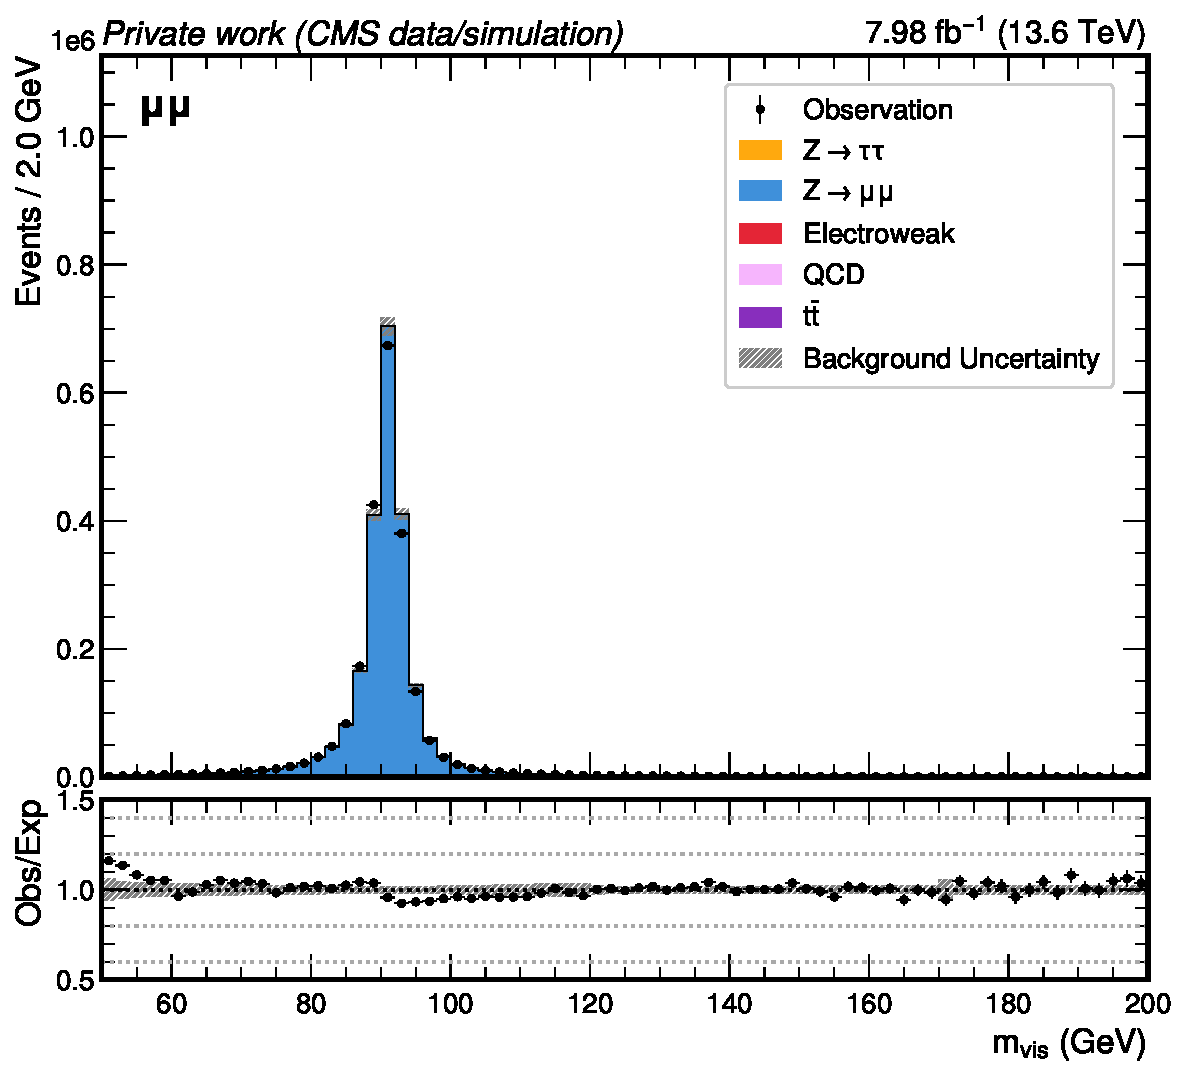
\includegraphics[width=\textwidth]{Figures/Chapter7/zpt_mvis_without.pdf}
            \caption{}
        \end{subfigure}
        \begin{subfigure}[b]{0.49\textwidth}
            \centering
            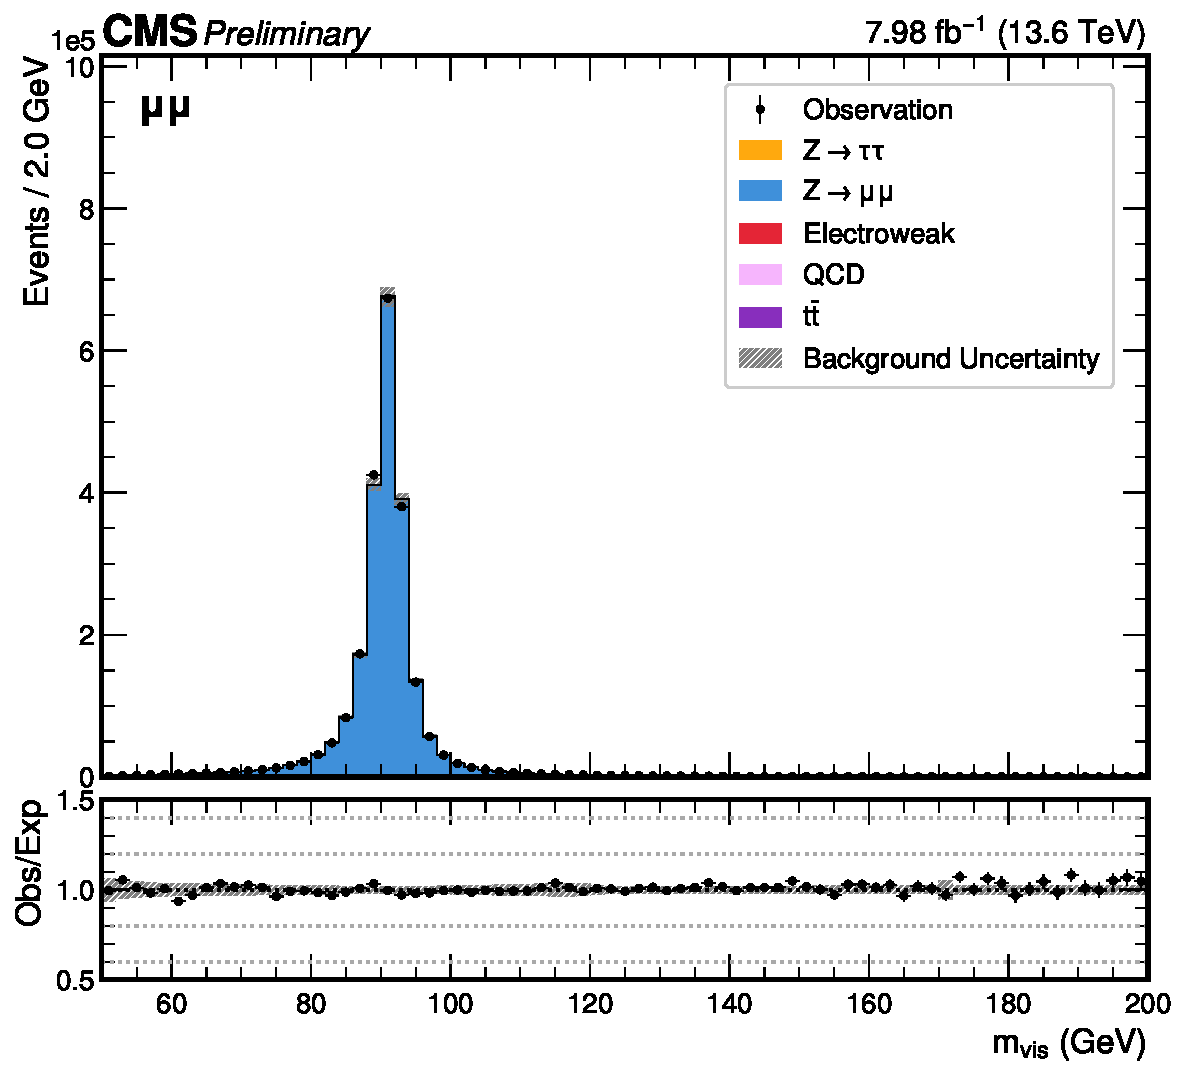
\includegraphics[width=\textwidth]{Figures/Chapter7/zpt_mvis_with.pdf}
            \caption{}
        \end{subfigure}

        \vspace{0.5cm}

        \begin{subfigure}[b]{0.49\textwidth}
            \centering
            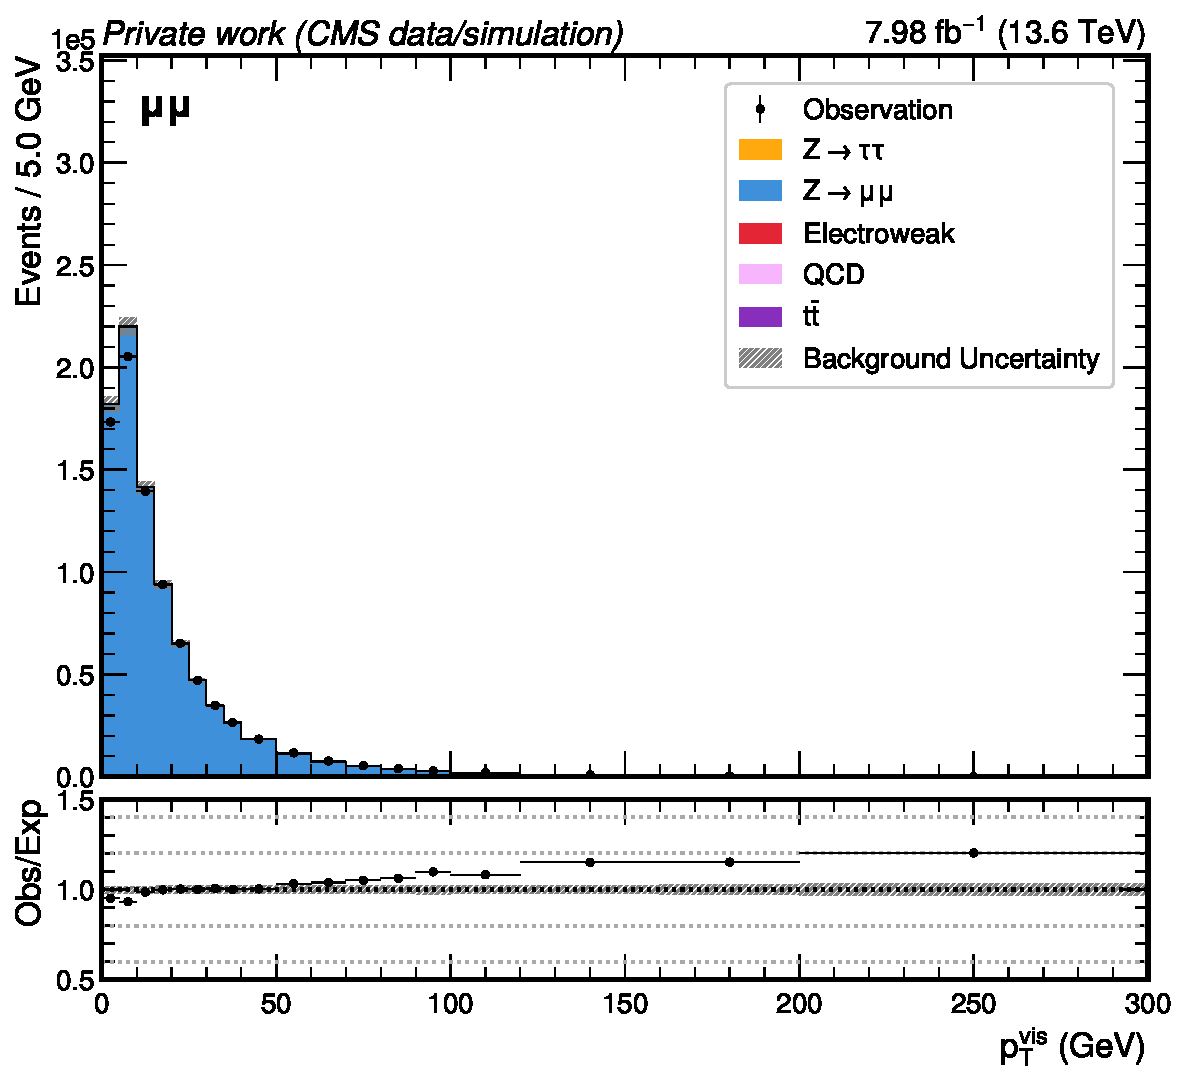
\includegraphics[width=\textwidth]{Figures/Chapter7/zpt_ptvis_without.pdf}
            \caption{}
        \end{subfigure}
        \begin{subfigure}[b]{0.49\textwidth}
            \centering
            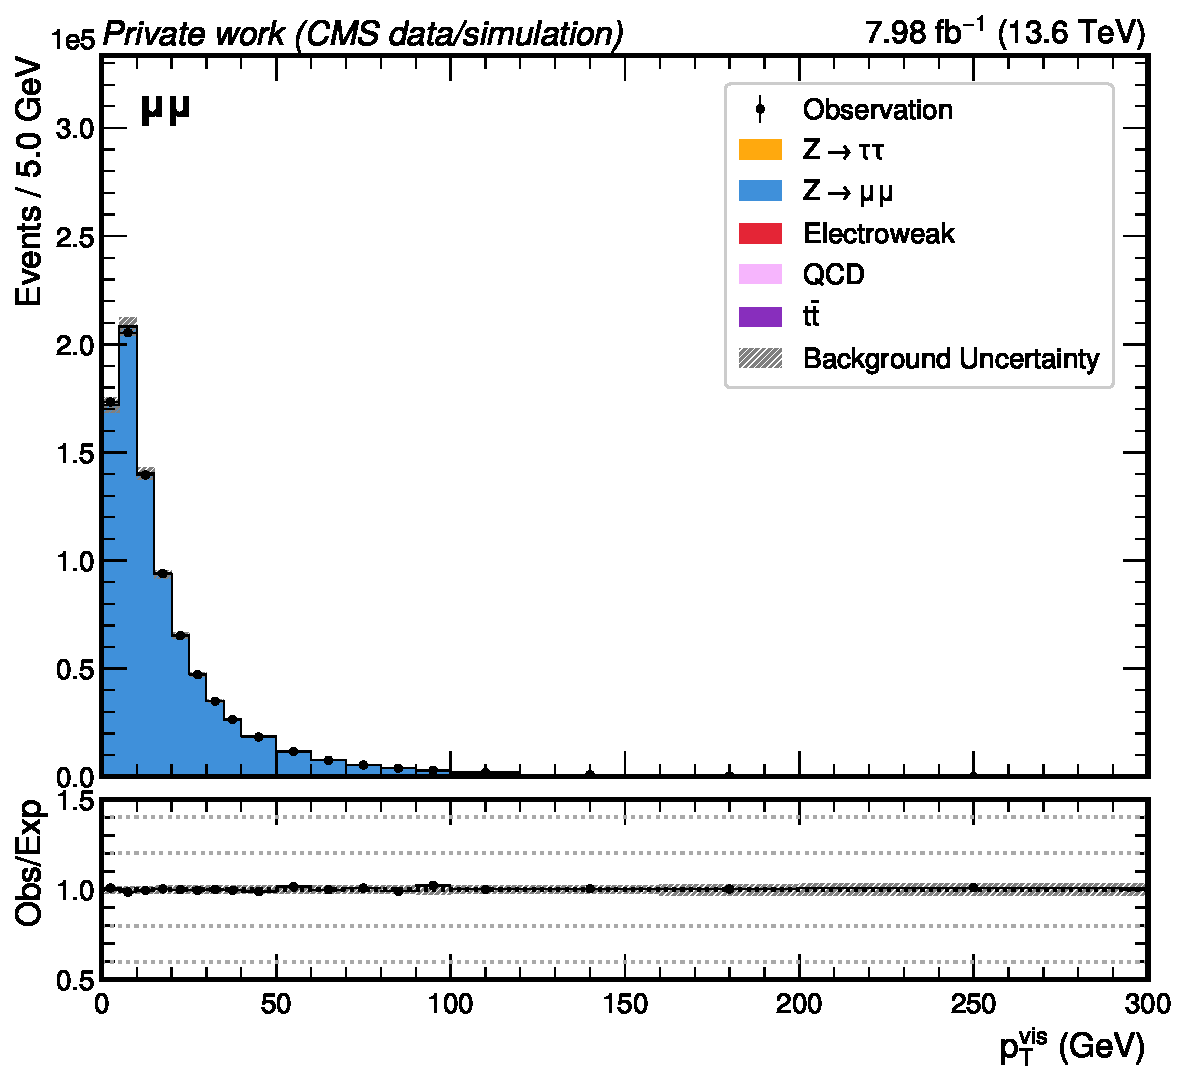
\includegraphics[width=\textwidth]{Figures/Chapter7/zpt_ptvis_with.pdf}
            \caption{}
        \end{subfigure}
    \caption[Reweighting validation in $Z/\gamma^* \to \mu\mu$ events.]{Validation of the $\PZ \, \, p_\text{T}$-mass reweighting in $Z/\gamma^* \to \mu\mu$ events. Shown are $m_\text{vis}$ distributions \textbf{(a)} before and \textbf{(b)} after reweighting, and $p_\text{T}^\text{vis}$ distributions \textbf{(c)} before and \textbf{(d)} after reweighting.}

    \label{Figure:Chapter6_ZPT_Reweighting}
\end{figure}

\begin{figure}[!htbp]
        \centering
        % First row
        \begin{subfigure}[b]{0.49\textwidth}
            \centering
            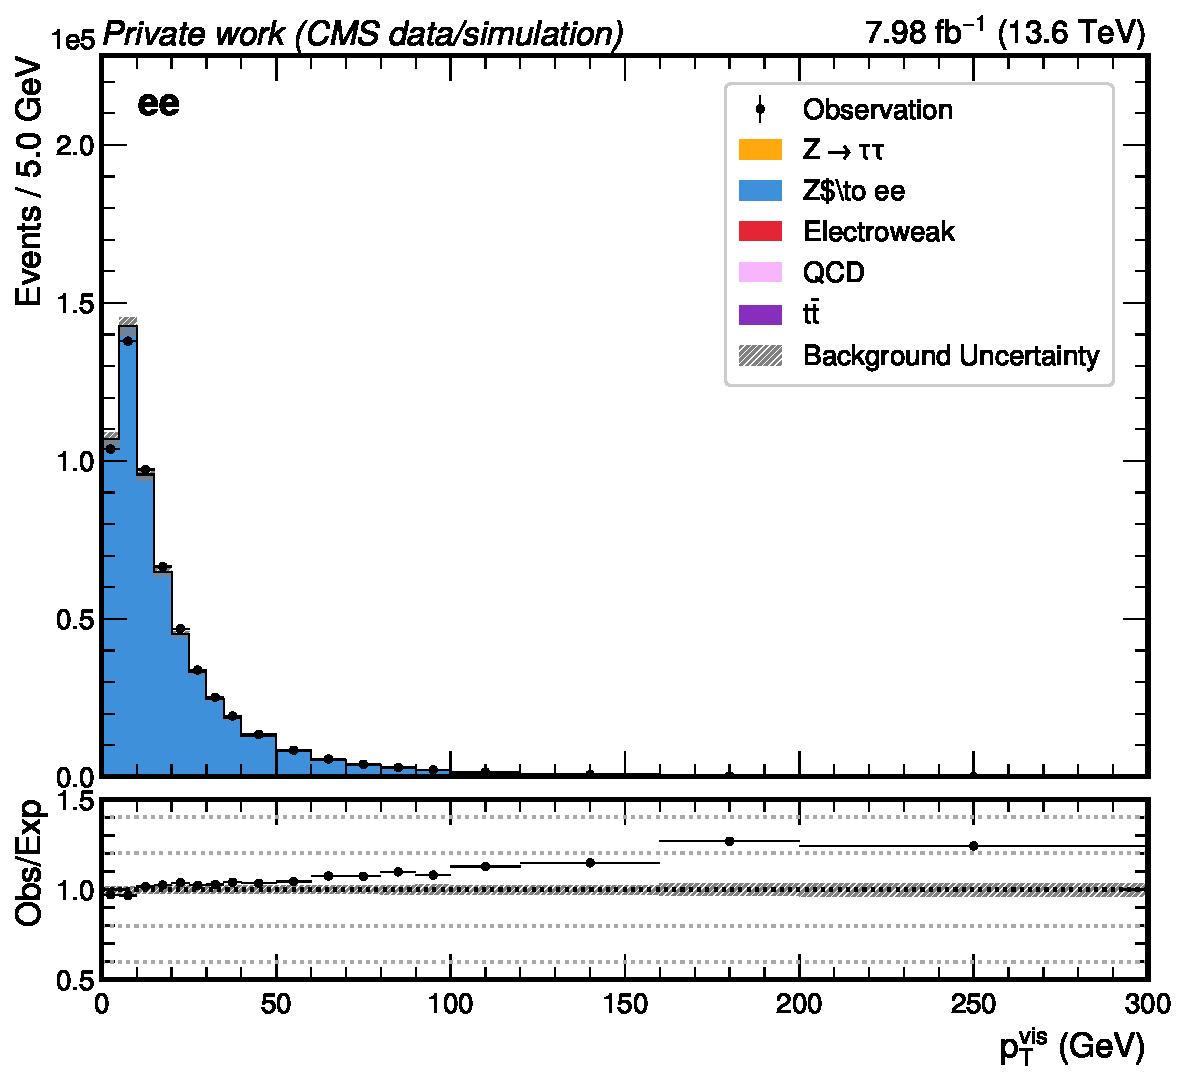
\includegraphics[width=\textwidth]{Figures/Chapter7/zpt_ee_ptvis_without.pdf}
            \caption{}
        \end{subfigure}
        \begin{subfigure}[b]{0.49\textwidth}
            \centering
            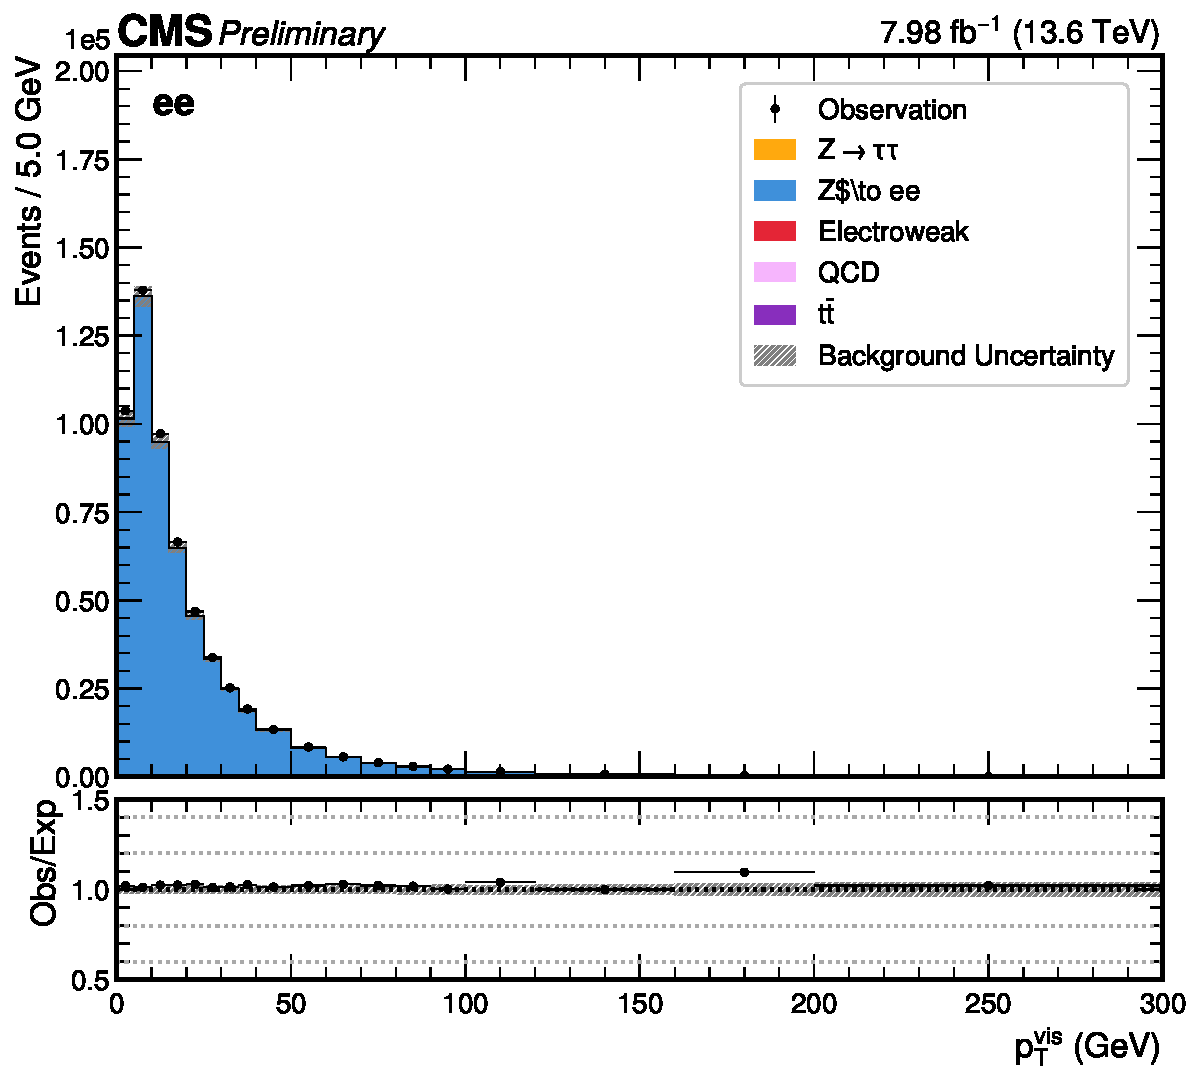
\includegraphics[width=\textwidth]{Figures/Chapter7/zpt_ee_ptvis_with.pdf}
            \caption{}
        \end{subfigure}
    \caption[Closure test of $\PZ \, \, p_\text{T}$-mass reweighting in $Z/\gamma^* \to ee$ events.]{Closure test of the $\PZ \, \, p_\text{T}$-mass reweighting in $Z/\gamma^* \to ee$ events. Distributions of $p_\text{T}^\text{vis}$ are shown \textbf{(a)} before and \textbf{(b)} after reweighting.}

    \label{Figure:Chapter6_ZPT_Reweighting_ee}
\end{figure}

\subsection{Top-quark \texorpdfstring{p$_\text{T}$}{pT} reweighting}

The simulation of $\ttbar$ production does not accurately reproduce the top-quark $p_\text{T}$ spectrum observed in data. To improve the agreement, dedicated event weights are applied. The weight is defined as

\begin{equation_pad}
    w = \sqrt{\text{SF}(p_\text{T}^{t}) \cdot \text{SF}(p_\text{T}^{\bar{t}})}
\end{equation_pad}
\begin{equation_pad}
    \text{SF}(p_\text{T}) = a \cdot e^{-b \cdot p_\text{T}} - c \cdot p_\text{T} + d,
\end{equation_pad}

where the parameters were determined from Run~2 data as $a = 0.103$, $b = 0.0118$, $c = 0.000134$, and $d = 0.973$~\cite{Czakon:2017wor}.

Since this parametrisation was derived at $\sqrt{s} = 13\TeV$, it must be extrapolated to the 13.6\TeV collision energy of Run 3. This is achieved by fitting the ratio of generator-level top-quark $p_\text{T}$ spectra between 13 and 13.6\TeV, resulting in an additional correction factor applied multiplicatively to the Run 2 parametrisation:

\begin{equation_pad}
    \text{SF}(p_\text{T}) = 0.991 + 0.000075 \, p_\text{T}
\end{equation_pad}

\subsection{IP Calibration}

As discussed in Section~\ref{Section:Chapter7_IP_METHOD}, the \ac{IP} vector is a key ingredient in reconstructing the $\PGt$ decay plane and, consequently, the CP-sensitive acoplanarity angle $\phi_{CP}$. Accurate modelling of the IP vector in simulation is therefore essential. Because the \ac{IP} vector is not perfectly modelled, a dedicated calibration is performed using clean samples of $Z \to \mu\mu$ and $Z \to ee$ events. 

Discrepancies between data and simulation in the Cartesian components of the \ac{IP} vector are corrected using the quantile mapping method. In this approach, the cumulative distribution of the uncalibrated simulation is mapped to that of the data, such that the corrected component of the \ac{IP} vector is defined as

\begin{equation_pad}
\mathrm{IP}_i^{\mathrm{corr}} = F^{-1}_{\mathrm{Data}}\!\left( F_{\mathrm{MC}}(\mathrm{IP}_i) \right)
\label{Equation:Chapter7_IP_Corr_1}
\end{equation_pad}

where $\mathrm{IP}_i^{\mathrm{corr}}$ and $\mathrm{IP}_i$ denote the corrected and uncorrected components of the IP vector, $F_{\mathrm{MC}}$ is the \ac{CDF} in simulation, and $F^{-1}_{\mathrm{data}}$ is the quantile function (inverse \ac{CDF}) in data. The procedure is illustrated schematically in Fig.~\ref{Figure:IP_QuantileMapping}.

\begin{figure}[!htbp]
    \centering
    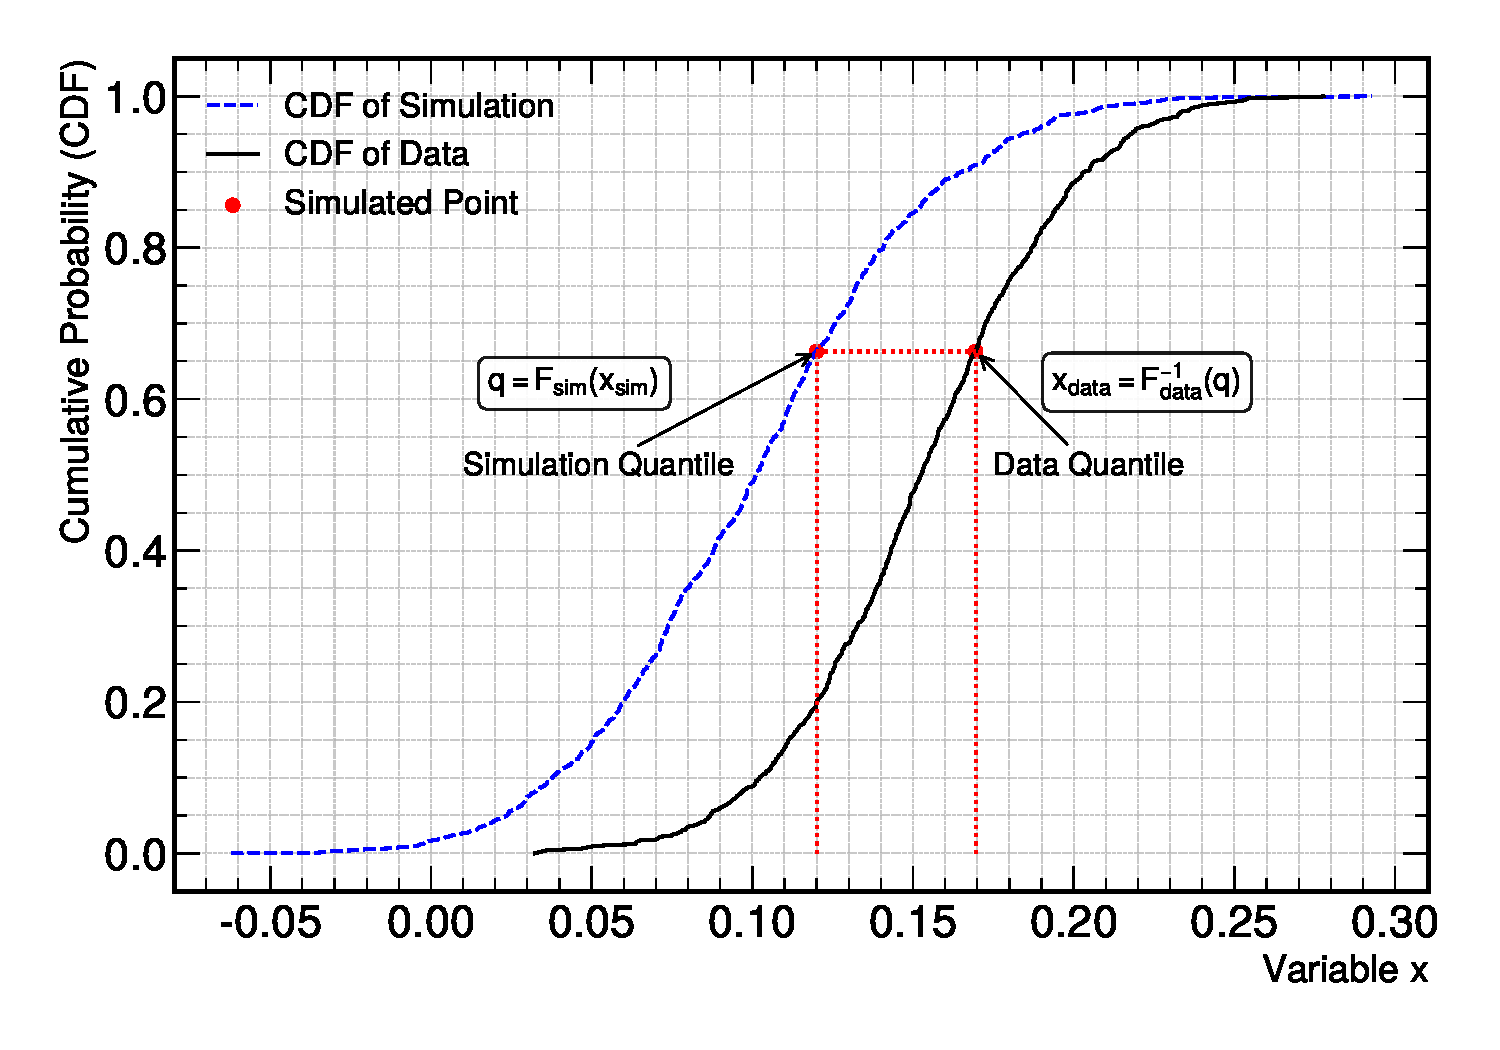
\includegraphics[width=0.7\textwidth]{Figures/Chapter7/quantile_mapping.pdf}
    \caption{Schematic representation of the quantile mapping procedure.}
    \label{Figure:IP_QuantileMapping}
\end{figure}

Because the IP resolution depends on track $\eta$, the correction is performed in bins of $|\eta|$ for both $Z \to \mu\mu$ and $Z \to ee$ events. An additional subtlety arises in the treatment of non-prompt particles. Equation~\ref{Equation:Chapter7_IP_Corr_1} is designed for prompt tracks, where the true \ac{IP} at generator level vanishes. Applying the same correction to non-prompt particles (\eg those from $\PGt$ decays) would distort their genuine decay length. To avoid this, the calibration is instead applied to the residual between the reconstructed and generator-level \ac{IP} vectors:


\begin{equation_pad}
\mathrm{IP}_i^{\mathrm{corr}} = \mathrm{IP}_i^{\mathrm{gen}} + F^{-1}_{\mathrm{Data}}\left( F_{\mathrm{MC}}\big(\mathrm{IP}_i - \mathrm{IP}_i^{\mathrm{gen}}\big) \right)
\end{equation_pad}

where $\mathrm{IP}_i^{\mathrm{gen}}$ is the generator-level component of the \ac{IP} vector.
This procedure ensures that the correction accounts for detector effects without biasing the genuine lifetime signatures of non-prompt particles. For prompt tracks, where $\mathrm{IP}_i^{\mathrm{gen}}=0$, the formula naturally reduces to the simpler form of Eq.~\ref{Equation:Chapter7_IP_Corr_1}. 

The effectiveness of the calibration is demonstrated in Fig.~\ref{Figure:IPvector_Corrections}, which compares data and simulation before and after applying the correction. Good closure is observed in both $Z\to ee$ and $Z\to\mu\mu$ control samples.

\begin{figure}[!htbp]
        \centering
        % First row
        \begin{subfigure}[b]{0.49\textwidth}
            \centering
            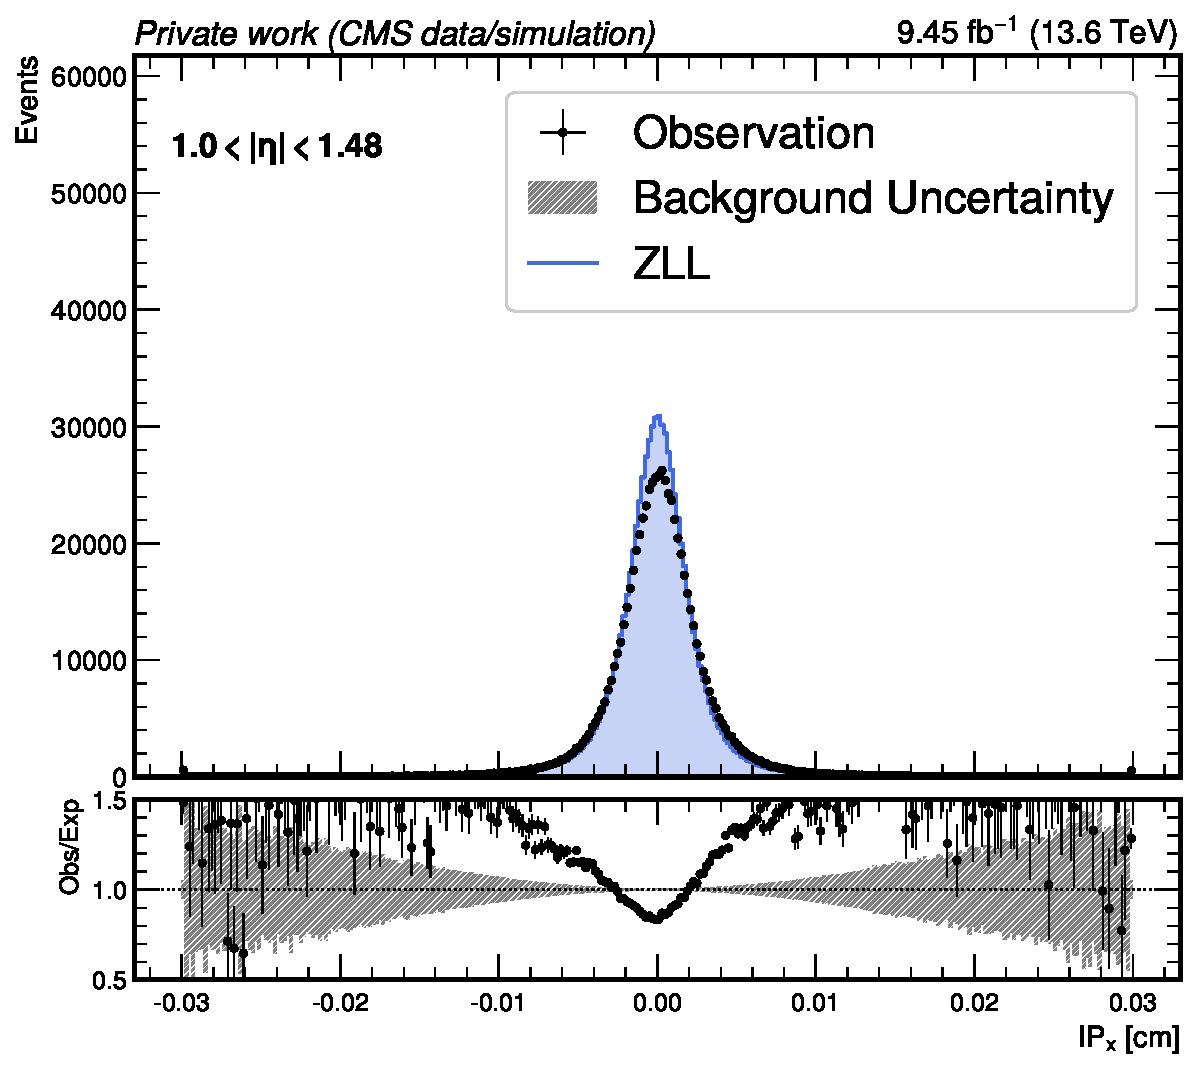
\includegraphics[width=\textwidth]{Figures/Chapter7/IP_Corrections/Before/ee/ip_x_1p0to1p48_comparison_with_ratio.pdf}
            \caption{}
        \end{subfigure}
        \begin{subfigure}[b]{0.49\textwidth}
            \centering
            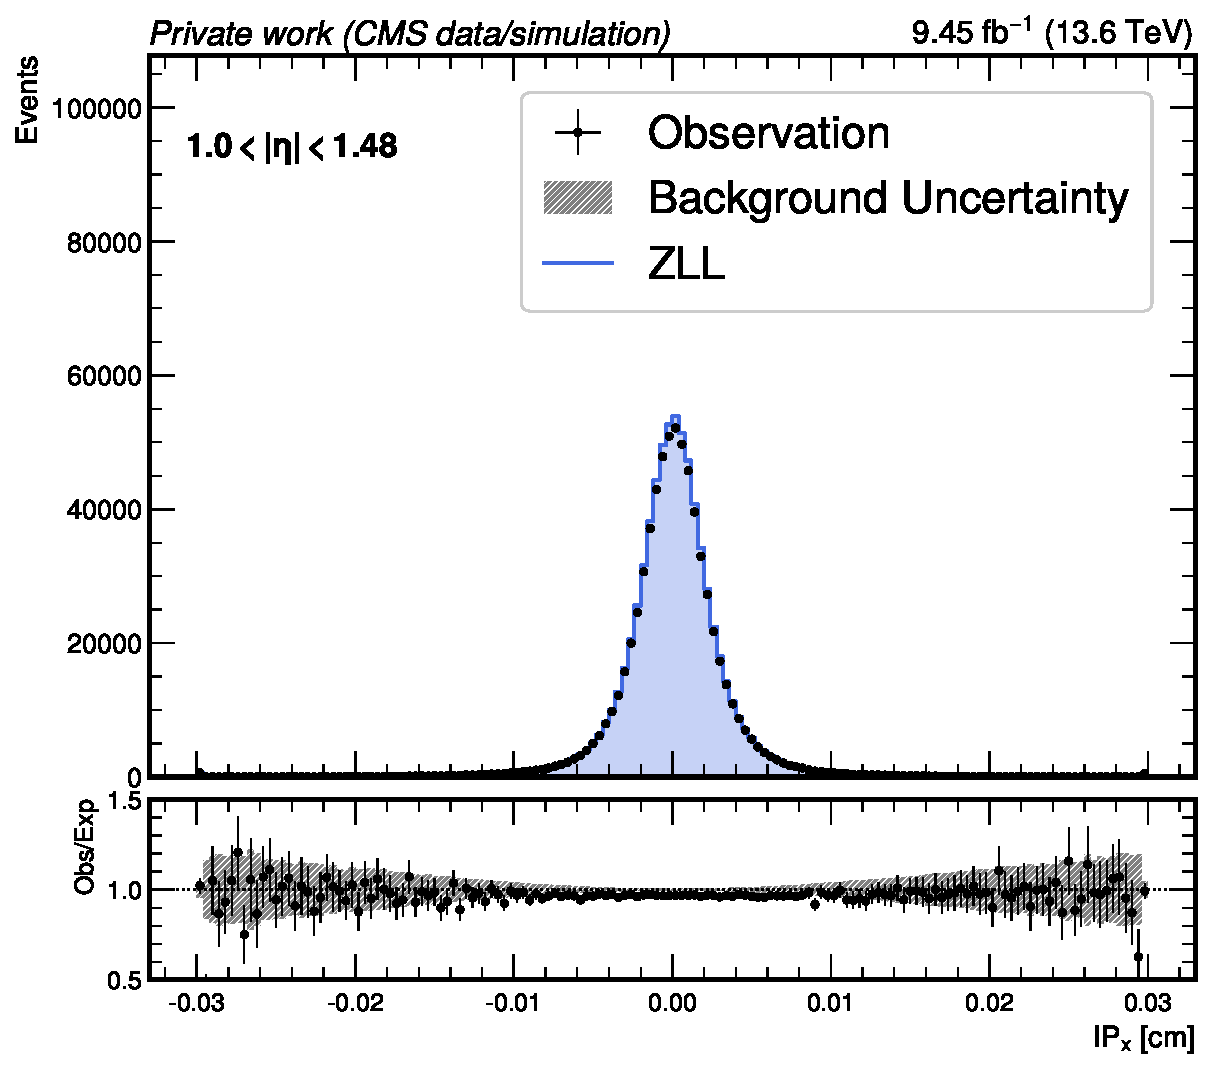
\includegraphics[width=\textwidth]{Figures/Chapter7/IP_Corrections/After/ee/ip_x_1p0to1p48_comparison_with_ratio.pdf}
            \caption{}
        \end{subfigure}

        \vspace{0.5cm}

        \begin{subfigure}[b]{0.49\textwidth}
            \centering
            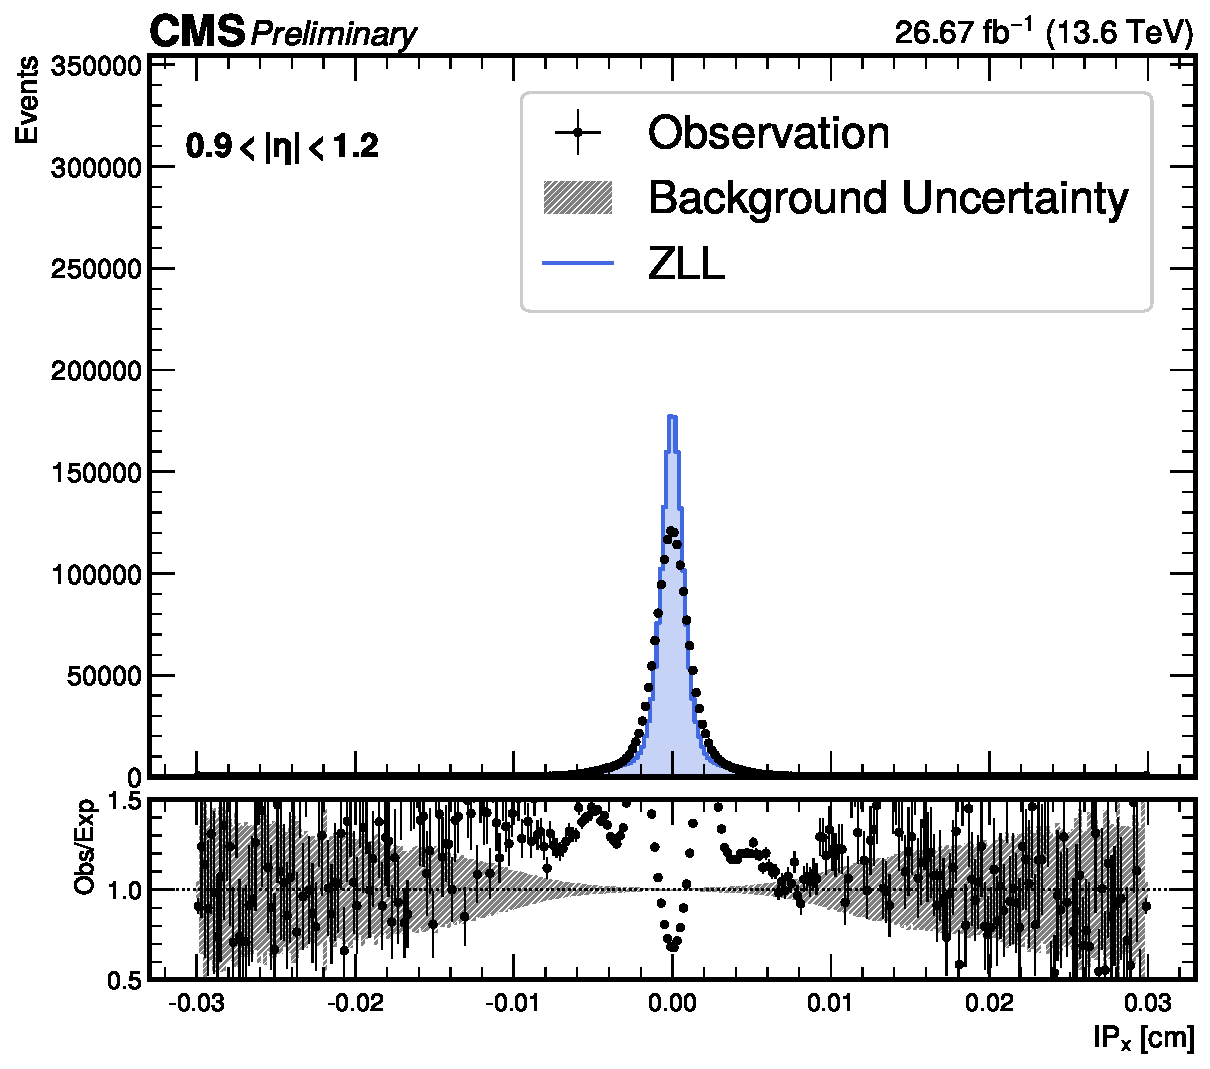
\includegraphics[width=\textwidth]{Figures/Chapter7/IP_Corrections/Before/mumu/ip_x_0p9to1p2_comparison_with_ratio.pdf}
            \caption{}
        \end{subfigure}
        \begin{subfigure}[b]{0.49\textwidth}
            \centering
            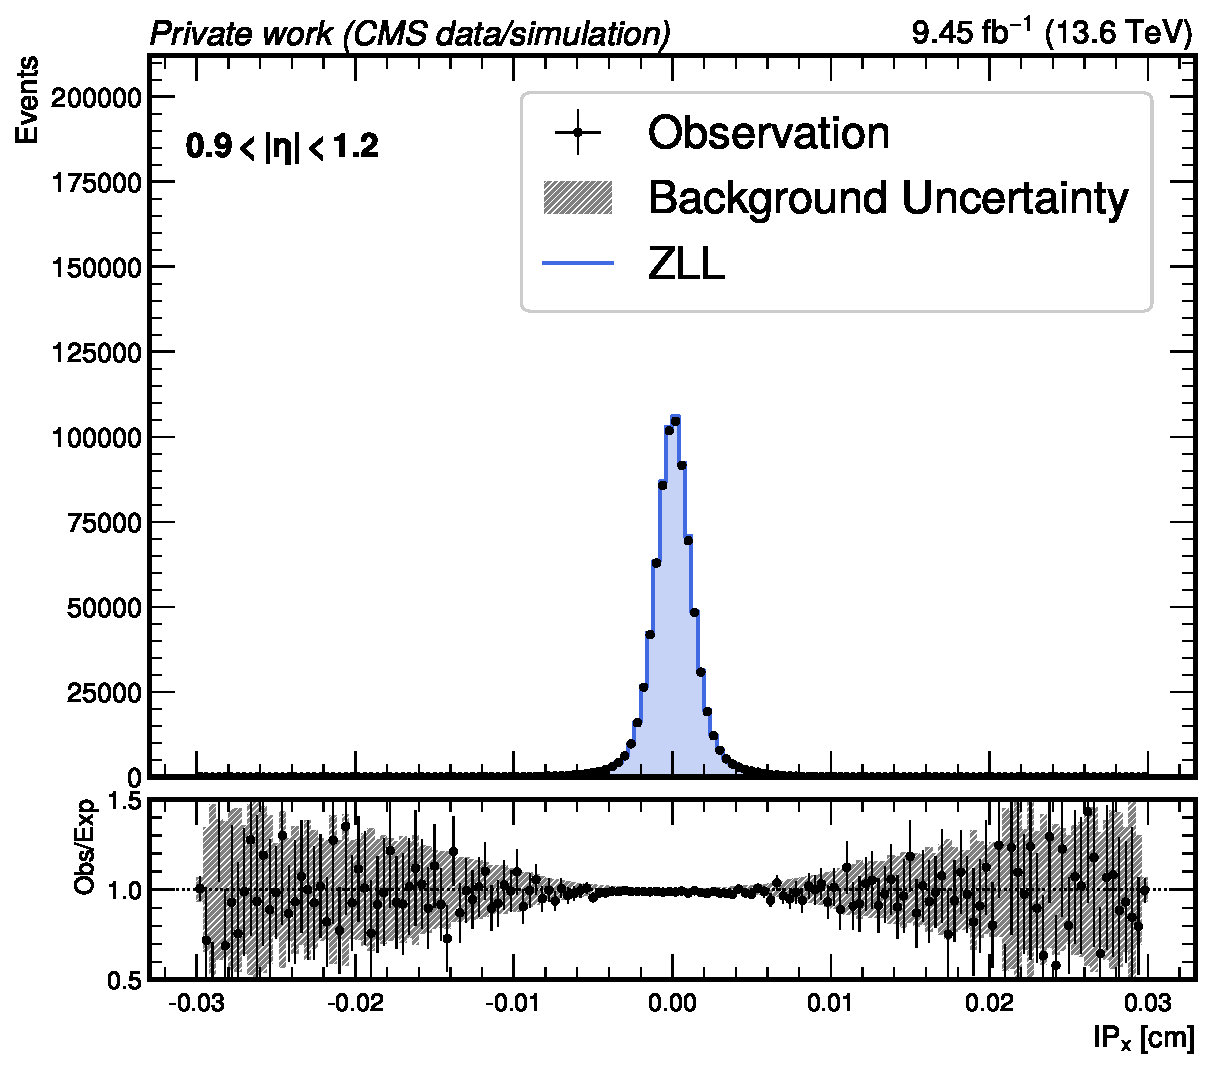
\includegraphics[width=\textwidth]{Figures/Chapter7/IP_Corrections/After/mumu/ip_x_0p9to1p2_comparison_with_ratio.pdf}
            \caption{}
        \end{subfigure}
    \caption[Validation of the IP calibration in $Z\to ee$ and $Z\to\mu\mu$ events.]
    {Validation of the \ac{IP} calibration using background-subtracted control samples of $Z\to ee$ and $Z\to\mu\mu$ events. 
    Distributions of the $x$ component of the IP vector are shown: \textbf{(a)} before and \textbf{(b)} after calibration in $Z\to ee$, 
    and \textbf{(c)} before and \textbf{(d)} after calibration in $Z\to\mu\mu$. }

    \label{Figure:IPvector_Corrections}
\end{figure}

The impact of the \ac{IP} calibration on the discriminating power of the acoplanarity angle observable is illustrated in Fig.~\ref{Figure:Chapter7_IPCalibration_Impact}. A slight reduction in the asymmetry between the CP-even and CP-odd scenarios is observed after applying the corrections, indicating that, prior to calibration, simulation overestimated the IP resolution.

\begin{figure}[!htbp]
        \centering
        % First row
        \begin{subfigure}[b]{0.49\textwidth}
            \centering
            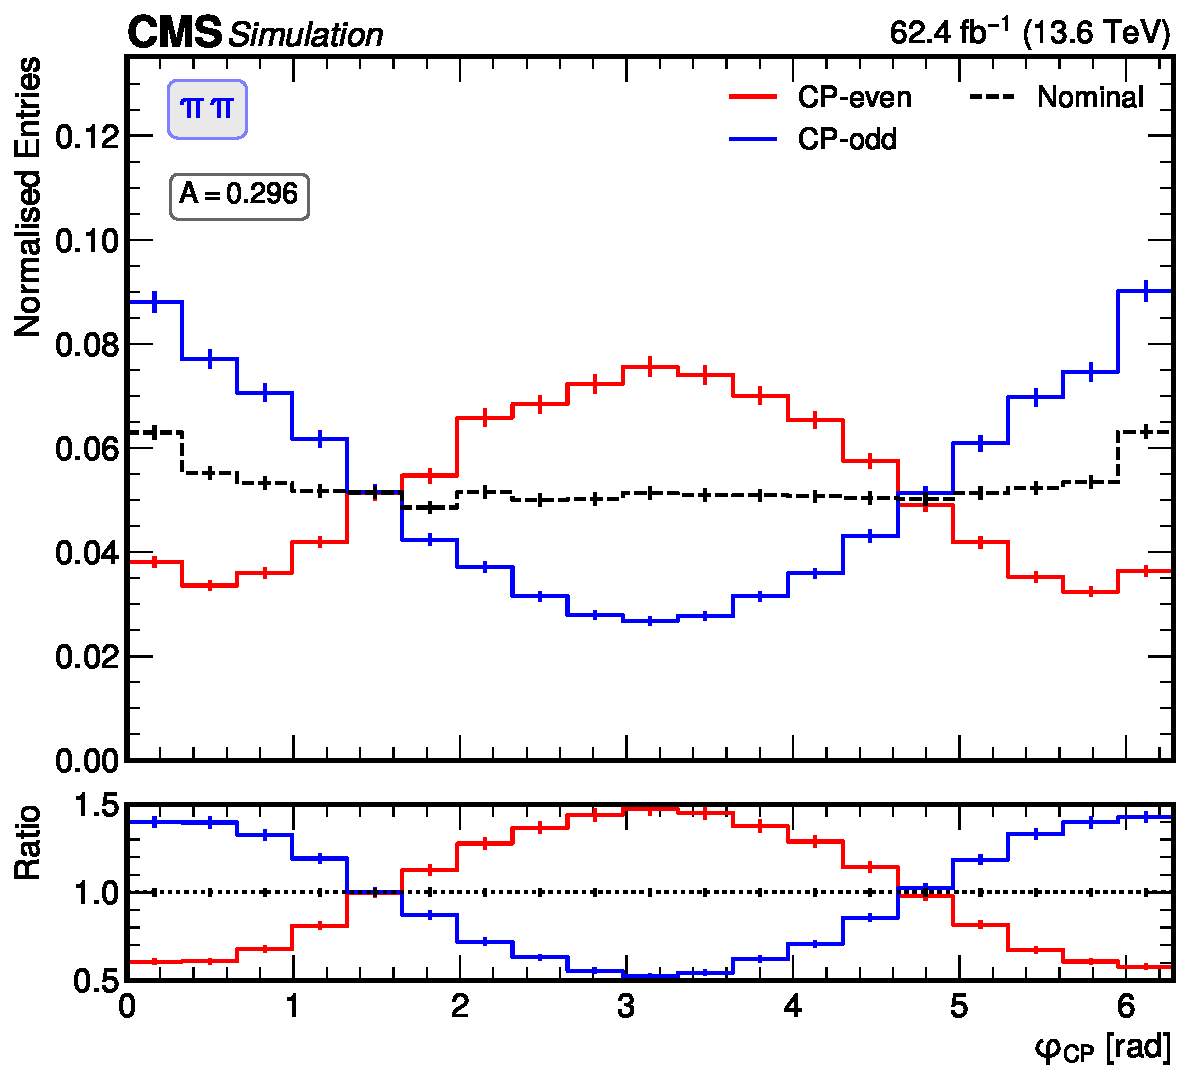
\includegraphics[width=\textwidth]{Figures/Chapter7/Acoplanarity/Without_IP/aco_pi_pi.pdf}
            \caption{}
        \end{subfigure}
        \begin{subfigure}[b]{0.49\textwidth}
            \centering
            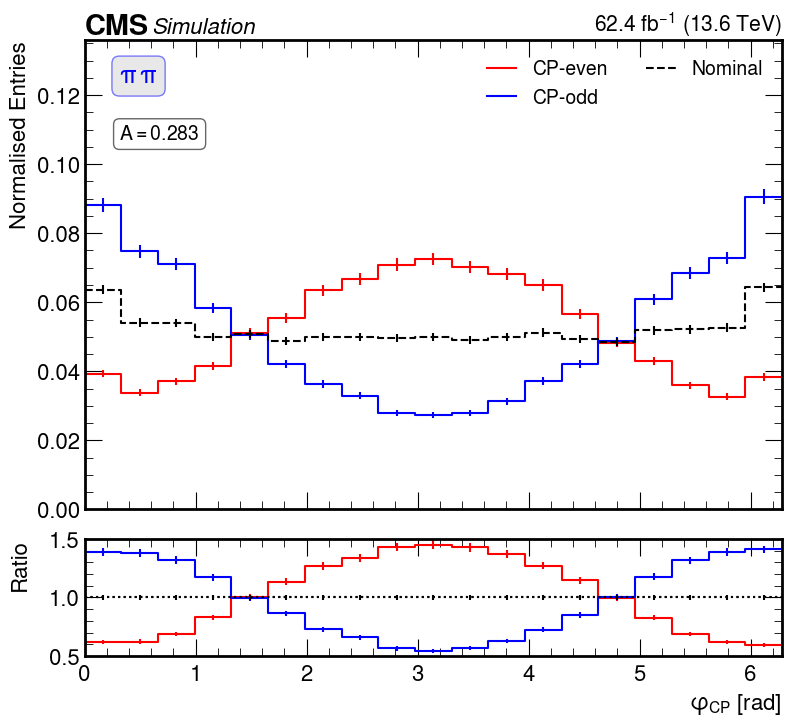
\includegraphics[width=\textwidth]{Figures/Chapter7/Acoplanarity/With_IP/aco_pi_pi.png}
            \caption{}
        \end{subfigure}

    \caption[Impact of the IP calibration on $\phi_{CP}$ reconstruction in $\pi\pi$ final states.]
    {Impact of the \ac{IP} calibration on the reconstructed $\phi_{CP}$ in the $\tauh\tauh \to \pi\pi$ final state. 
    Distributions are shown \textbf{(a)} before and \textbf{(b)} after applying the calibration to the IP vector.}
    \label{Figure:Chapter7_IPCalibration_Impact}
\end{figure}

\subsection{\texorpdfstring{$\vec{E}^{\text{miss}}_\text{T}$}{ET miss} recoil}

To improve the modelling of $\vec{E}_T^\text{miss}$, recoil corrections are applied to selected simulated samples. A source of mismodelling arises from the hadronic recoil, defined as

\begin{equation_pad}
    \vec{U}_\text{T} =  \vec{E}_T^\text{miss} - \sum_\nu p_\text{T}^\nu
\end{equation_pad}

where the sum runs over all neutrinos in the event. The hadronic recoil is determined using a sample of $Z \to \mu\mu$ events by measuring the $p_\text{T}$ of the $Z$ boson, $p_\text{T}^\PZ$, and the total transverse momentum of the recoiling jets, $\vec{H}_\text{T}$. In this case, no neutrinos are present, so the hadronic recoil coincides with the reconstructed $\vec{E}_T^\text{miss}$ and can be written as

\begin{equation_pad}
    \vec{U}_\text{T} = -\vec{H}_T - p_\text{T}^\PZ \equiv \vec{E}_T^\text{miss}
\end{equation_pad}

The recoil is decomposed into components parallel and perpendicular to the $\PZ$ boson direction in the transverse plane, and distributions of $U_\parallel$ and $U_\perp$ are constructed in bins of $p_\text{T}^\PZ$ and jet multiplicity, both in data and simulation. From these histograms, the corresponding \acp{CDF} are derived:

\begin{equation_pad}
F_\text{Data/MC}(U_{\parallel/\perp}) = \int_{-\infty}^{U_{\parallel/\perp}} f_\text{Data/MC}(x) \,\, dx
\end{equation_pad}

A simulated recoil value $U$ is then corrected by quantile mapping:

\begin{equation_pad}
U_{\parallel/\perp}^\prime = F_\text{data}^{-1}\big(F_\text{MC}(U)\big)
\end{equation_pad}

This procedure transforms the simulated recoil distribution to match that observed in data. The corrected parallel and perpendicular components are propagated back into the computation of $\vec{E}_T^\text{miss}$, leading to improved agreement between data and simulation in observables sensitive to $\vec{E}_T^\text{miss}$.

\subsection{ggH quark-mass effects}

Corrections for finite top-quark mass effects are applied to account for the limitations of the large-$m_t$ approximation in gluon-fusion Higgs production. In this approximation, the top-quark loop is replaced by an effective pointlike interaction, which provides an accurate description of the inclusive cross section but fails to capture the correct $m_t$ dependence at high Higgs transverse momentum. At $p_\text{T}^H \gtrsim m_t$, the internal loop structure becomes resolved, and the approximation tends to overestimate the cross section. To recover the correct kinematic behaviour, differential reweighting factors are obtained using \textsc{HRes}~\cite{deFlorian:2012mx,Grazzini:2013mca}, which computes the Higgs $p_\text{T}$ spectrum both in the large-$m_t$ limit and with exact top-mass dependence. The ratio of the two predictions is used to reweight simulated events, thereby restoring the correct mass dependence in the high-$p_\text{T}$ region.

\section{Background modelling}
\label{Section:Chapter7_Background_Modelling}

Background contributions in the $\tauh\tauh$ channel are categorised into three classes:

\begin{enumerate}[label=(\roman*)]
\item \textbf{Genuine-$\PGt$ backgrounds:} Events with two genuine $\tauh$ candidates. This class is dominated by $\PZ/\gamma^*\!\to\!\tau\tau$, with smaller contributions from $\ttbar$ and diboson production. These processes are estimated using simulation.
\item \textbf{Jet$\to\tauh$ misidentification:} Events in which one or more jets are misidentified as $\tauh$. This background is estimated with a data-driven $F_F$ method.
\item \textbf{Lepton$\to\tauh$ misidentification:} Events in which electrons or muons are misidentified as $\tauh$. This contribution is largely suppressed by the dedicated anti-$e/\mu$ discriminators and is subdominant. It is estimated from simulation.
\end{enumerate}

\subsection{\texorpdfstring{Background from Jets Misidentified as $\PGt_h$ (Jet $\to \PGt_h$)}{Background from Jets Misidentified as hadronic taus}}
\label{Section:Chapter7_FF}

As discussed in Section~\ref{Section:Chapter6_JetToTauBackground}, MC simulation does not provide a reliable description of the jet$\to\tauh$ misidentification rate. Therefore, a $F_F$ method is employed. In this channel, a simplified implementation, closer to the Classical $F_F$ approach (Section~\ref{Section:Chapter6_FakeFactors_Classical}), is adopted instead of the \ac{ML}-based reweighting strategy of Section~\ref{Section:Chapter6_FakeFactors_BDT}. 

In brief, the method estimates the jet$\to\tauh$ contribution in the \ac{SR} by extrapolating from a sideband region defined by looser $\tauh$ identification criteria. The raw $F_F$ is computed as the ratio of events passing the nominal ID to those failing the nominal ID but passing a looser selection (Equation~\ref{Equation:Chapter6_FF}). The \ac{WP} used to define these regions are summarised in Table~\ref{Table:Chapter7_Tauh_SelectionSummary}.

Once derived, the $F_F$ is corrected using dedicated closure and extrapolation factors. These account for differences between the signal and determination regions, as well as the limited parameterisation of the misidentification rate. The corrected $F_F$ is then applied to events in the \ac{SR} that fail the nominal ID but pass the alternative ID, yielding an estimate of the jet$\to\tauh$ background. As noted in Section~\ref{Section:Chapter6_FakeFactors_Classical}, the $F_F$ is measured only for the leading $\tauh$ candidate. As a result, events where the leading $\tauh$ is genuine but the subleading candidate is a misidentified jet are not captured by the method. These subdominant contributions are taken from simulation and added to the estimate.

\section{Uncertainty model}
\label{Section:Chapter7_UncertaintyModel}

The treatment of uncertainties in this chapter follows the same principles as in Section~\ref{Section:Chapter6_Uncertainty_Model}, with modifications reflecting the specifics of this analysis. Some sources are treated identically and are only listed here for completeness, with references to the corresponding sections for details:

\begin{itemize}
  \item \textbf{Luminosity:} For the combined data-taking eras, the highest uncertainty across years (1.4\%) is used. It is implemented as a normalisation-only uncertainty.
  \item \textbf{Hadronic tau efficiencies:} Identification and energy scale efficiencies are treated identically to Section~\ref{Section:Chapter6_UModel_HadronicTau}.
  \item \textbf{Jet energy scale and resolution:} Treated as in Section~\ref{Section:Chapter6_UModel_Jets}. The energy scale of the unclustered component of $E_{\mathrm{T}}^{\text{miss,PF}}$ is not considered in this analysis.
\end{itemize}


\subsection{Trigger efficiencies}

Uncertainties for the $\tau\tau$ and $\tau\tau$+jet triggers are implemented as shape variations. For the $\tauh$ legs, per-DM and per-era uncertainties are assigned independently for each trigger. For the $\tauh{+}$jet path, an additional independent jet-leg shape uncertainty is included, which is also decorrelated across data-taking eras. 

\subsubsection{Top- and Z-boson reweighting}
For both the $t\bar{t}$ and $\PZ/\gamma^\ast \to \ell^+\ell^-$ backgrounds, uncertainties are assigned to the applied reweighting corrections.  
Each is implemented as shape variations, corresponding to omitting the correction entirely or applying it twice, which represents a conservative 100\% uncertainty in the reweighting procedure.

\subsubsection{IP Calibration}
A systematic uncertainty is assigned to the correction of the \ac{IP} vector.  
The corrected value, $\mathrm{IP}^{\text{corr}}_{\text{sig}}$, is shifted up and down by one quarter of the difference between the corrected and uncorrected values, $\mathrm{IP}^{\text{uncorr}}_{\text{sig}}$:  
\begin{align}
\mathrm{IP}^{\text{up}}_{i}   &= \mathrm{IP}^{\text{corr}}_{i} + 0.25 \, \left(\mathrm{IP}^{\text{corr}}_{i} - \mathrm{IP}^{\text{uncorr}}_{i}\right) \\
\mathrm{IP}^{\text{down}}_{i} &= \mathrm{IP}^{\text{corr}}_{i} - 0.25 \, \left(\mathrm{IP}^{\text{corr}}_{i} - \mathrm{IP}^{\text{uncorr}}_{i}\right)
\end{align}

This uncertainty accounts for residual mismodelling observed in the distributions of the \ac{IP} components between simulation and data in $Z \to ee/\mu\mu$ events. It is implemented as a shape variation, but its impact on the $\phi_{\text{CP}}$ distribution is expected to be small, as illustrated in Fig.~\ref{Figure:CPDist_IPCalibration_Unc}.

\begin{figure}[!htbp]
    \centering
    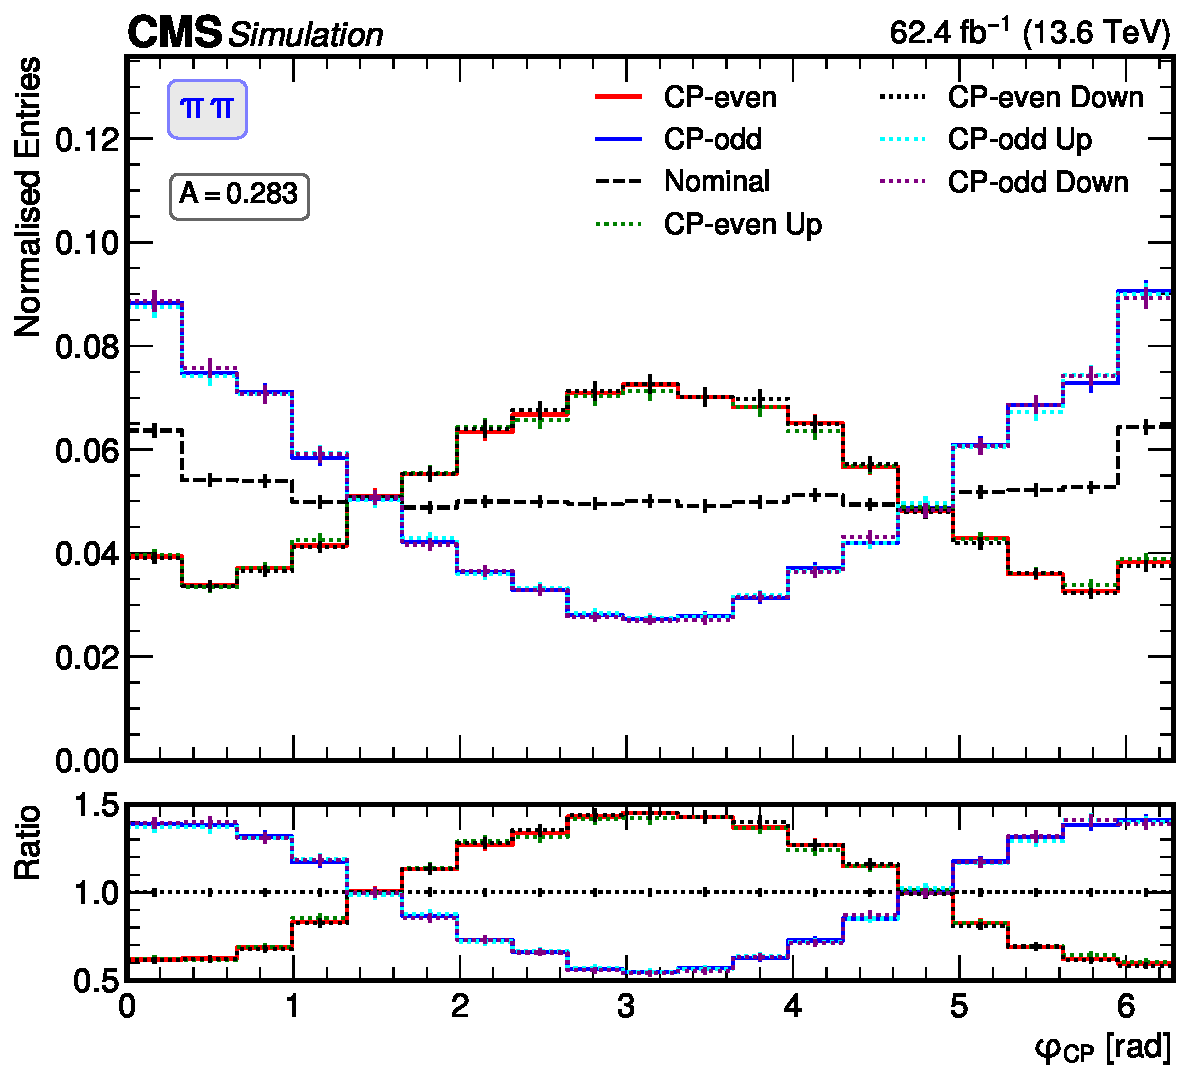
\includegraphics[width=0.6\textwidth]{Figures/Chapter7/Acoplanarity/Angular_Systematics/aco_pi_pi.pdf}
    \caption{Impact of IP vector calibration uncertainty on $\phi_{CP}$ distribution in the $\pi\pi$ category.}
    \label{Figure:CPDist_IPCalibration_Unc}
\end{figure}

\subsubsection{Secondary vertex reconstruction}

A systematic uncertainty is assigned to account for potential mis-reconstruction of the \ac{SV}, which can bias the acoplanarity angle $\phi_{\text{CP}}$.  
To evaluate this effect, an alternative value of $\phi_{\text{CP}}$ is computed by rotating the \ac{SV} towards or away from the generator-level position.  
Based on the variations observed from this procedure, a conservative 20\% uncertainty is assigned.  Its impact on the $\phi_{\text{CP}}$ distribution is, however, found to be minimal, as illustrated in Fig.~\ref{Figure:CPDist_SVCalibration_Unc}.  
This uncertainty is implemented as a shape variation.

\begin{figure}[!htbp]
    \centering
    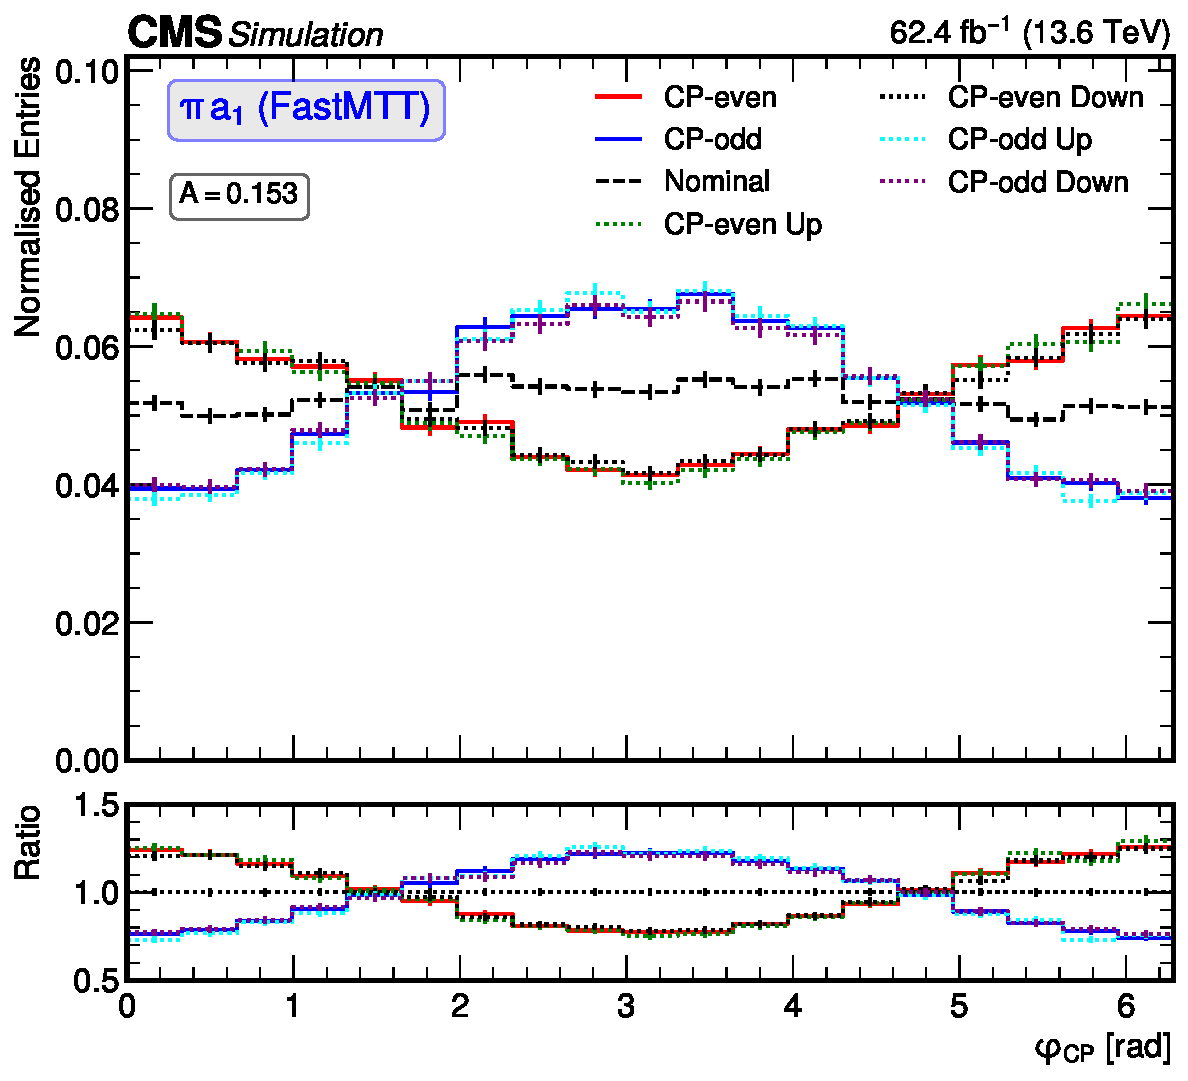
\includegraphics[width=0.6\textwidth]{Figures/Chapter7/Acoplanarity/Angular_Systematics/aco_pi_a1_FASTMTT_MassConstraint.pdf}
    \caption{Impact of SV calibration uncertainty on $\phi_{CP}$ distribution in the $\pi a_1^\text{3pr}$ category.}
    \label{Figure:CPDist_SVCalibration_Unc}
\end{figure}

\subsection{\texorpdfstring{$\vec{E}^{\text{miss}}_\text{T}$}{ET miss} recoil}

Uncertainties in the recoil corrections are derived from residual differences between data and simulation in $\PZ \to ee$ control samples. After the nominal recoil corrections are applied, two components are considered:  

\begin{itemize}
  \item \textbf{Response:} Projection of the hadronic recoil along the boson direction, normalised to the boson $p_\text{T}$.  
  \item \textbf{Resolution:} Projection of the hadronic recoil perpendicular to the boson direction, again normalised to the boson $p_\text{T}$.  
\end{itemize}

The uncertainties are obtained by comparing the mean of the response distribution and the width of the resolution distribution in data and simulation.  
The observed differences are taken as systematic variations and propagated to the reconstructed $\vec{E}^{\text{miss}}_\text{T}$. These variations are applied as shape uncertainties to all processes for which recoil corrections are used.

\subsection{Cross-section uncertainties}
Uncertainties in the production cross sections of major background processes are treated as normalisation-only effects and are summarised in Table~\ref{Table:Chapter7_XS_Uncertainties}.  

\begin{table}[!htbp]
\centering
\renewcommand{\arraystretch}{1.5}
\setlength{\tabcolsep}{12pt} % Increase column width
\begin{tabular}{l c c}
\hline
Process & Source & Uncertainty \\
\hline
DY & QCD scale + PDF + Scheme & --1.6\% / +1.3\%~\cite{Grazzini:2017mhc} \\
$t\bar{t}$ & QCD scale + PDF + $\alpha_s$ & --5.1\% / +4.4\%~\cite{Czakon:2011xx,Botje:2011sn} \\
Diboson, rare & QCD scale + PDF + Scheme & $\pm$5\%~\cite{Grazzini:2017mhc} \\
\arrayrulecolor{lightgray}\hline
\multirow{6}{*}{Higgs production} 
& \multirow{3}{*}{QCD scale} 
  & $\pm$3.9\% (ggH)~\cite{Karlberg:2024zxx} \\
&  & --0.7\% / +0.4\% (WH)~\cite{Karlberg:2024zxx} \\
&  & --3.2\% / +3.8\% (ZH)~\cite{Karlberg:2024zxx} \\
& \multirow{3}{*}{PDF} 
  & $\pm$3.2\% (ggH, VBF)~\cite{Karlberg:2024zxx} \\
&  & $\pm$1.6\% (WH)~\cite{Karlberg:2024zxx} \\
&  & $\pm$1.3\% (ZH)~\cite{Karlberg:2024zxx} \\
\arrayrulecolor{lightgray}\hline
\multirow{3}{*}{Higgs BR ($H\to\tau\tau$)} 
& Theoretical & --1.6\% / +1.7\%~\cite{MelladoGarcia:2150771}\\
& \multirow{2}{*}{Parametric} & $\pm$1.0\% ($m_q$)~\cite{MelladoGarcia:2150771} \\
&  & $\pm$0.6\% ($\alpha_s$)~\cite{MelladoGarcia:2150771} \\
\arrayrulecolor{black}\hline
\end{tabular}
\caption{Summary of cross-section and branching ratio uncertainties.}
\label{Table:Chapter7_XS_Uncertainties}
\end{table}

\subsubsection{Signal theory uncertainties}
In this analysis, theoretical uncertainties in the signal modelling are limited to QCD scale and \ac{PDF} variations. Both are implemented as shape uncertainties.

\subsection{Jets \texorpdfstring{$\to \PGt_h$}{to hadronic tau} background}

The following uncertainty components are assigned to the jet$\to \PGt_h$ estimate:
\begin{itemize}
    \item \textbf{Statistical:} Fitted parameters of the $F_F$ are propagated as shape variations, decorrelated by \ac{DM}.
    \item \textbf{Alternative validation region:} A dedicated validation region is defined by inverting the ID requirement on the subleading $\tauh$. The associated uncertainties are separated into the following components:
    \begin{enumerate}
        \item \textbf{Overall normalisation:} Derived in a distribution binned simultaneously by \ac{BDT} score\footnote{Here the \ac{BDT} score refers to the output of the signal-background classifier introduced in Section~\ref{Section:Chapter7_EventCategorisation}.} and $\phi_{CP}$. This accounts for residual differences observed between data and prediction in the validation region. 
        \item \textbf{\ac{BDT} score:} Shape uncertainty assigned since the $F_F$ is not derived as a function of the \ac{BDT} discriminant.  
        \item \textbf{$\phi_{CP}$:} Shape uncertainty assigned since the $F_F$ is not derived as a function of the acoplanarity angle.  
    \end{enumerate}
    \item \textbf{Subtracted real-$\tau$ contamination:} A shape uncertainty is assigned to account for the subtraction of genuine-$\tau$ backgrounds in the control regions. In addition, a 30\% normalisation uncertainty is applied to the simulated contribution in events where the subleading $\tau$ candidate is misidentified and the leading $\tau$ candidate is genuine.
\end{itemize}

\section{Statistical procedure}
\label{Section:Chapter7_StatisticalProcedure}
The extraction of the CP effective mixing angle $\alpha_{\PH\tau\tau}$ is performed via a simultaneous binned maximum-likelihood fit to the distribution of the discriminating observable in all categories. The likelihood function, denoted by $\mathcal{L}$, is defined as,

\begin{equation}
\mathscr{L}(\text{data} \,|\, \mu_{\tau\tau}, \alpha_{\PH\tau\tau}, \theta) 
= \prod_{i=1}^{N_\text{c}} 
\text{Poisson}\!\left( 
n_i \,\middle|\,  S_i(\mu_{\tau\tau}, \alpha_{\PH\tau\tau}, \theta)
+ B_i(\theta) 
\right) \cdot p(\hat{\theta} \,|\, \theta),
\label{eq:likelihood_alpha}
\end{equation}

where:
\begin{itemize}
    \item $n_i$ is the number of observed events in bin $i$ of the fit, with $i$ running over all bins in all categories.
    \item $\mu_{\tau\tau}$ is a signal strength parameter, scaling the total Higgs boson production cross section multiplied by the branching fraction $\text{B}_f(H\to\tau\tau)$ relative to the \ac{SM} prediction. This parameter $\mu_{\tau\tau}$ is left unconstrained in the fit, such that the normalisation of the signal is determined from data. 
    This ensures that the extraction of $\alpha_{\PH\tau\tau}$ relies solely on the shape of the $\phi_{\mathrm{CP}}$ distribution, rather than on the absolute rate.
    \item $S_i(\mu_{\tau\tau}, \alpha_{\PH\tau\tau}, \theta)$ and $B_i(\theta)$ denote the expected signal and background yields in bin $i$, respectively. 
    \item $\theta$ is the set of nuisance parameters, corresponding to the systematic uncertainties described in Section~\ref{Section:Chapter7_UncertaintyModel}.
    \item $p(\hat{\theta} \,|\, \theta)$ encodes the set of \acp{P.D.F} constraining the nuisance parameters to their nominal values (see discussion in Section~\ref{Section:Chapter6_NuisanceParameters}).
\end{itemize}

The best-fit value of $\alpha_{\PH\tau\tau}$ is obtained by maximising the likelihood. 
Confidence intervals are constructed using the negative log-likelihood ratio,

\begin{equation}
-2\Delta\ln\mathscr{L}(\alpha_{\PH\tau\tau}) = -2\ln\frac{\mathscr{L}(\alpha_{\PH\tau\tau})}{\mathscr{L}(\hat{\alpha}_{\tau\tau})}
\end{equation}

where $\hat{\alpha}_{\tau\tau}$ denotes the best-fit value of the parameter of interest $\alpha_{\PH\tau\tau}$
The values of $-2\Delta\ln\mathcal{L}$ equal to 1.00, 4.02, and 8.81 correspond to the $68.3\%$, $95.5\%$, and $99.7\%$ CL, respectively.

\section{Measurement optimisation}
\label{Section:Chapter7_Optimisation}
The sensitivity of the measurement is maximised through a series of optimisation studies. These studies include the choice of event categorisation, the selection criteria applied to the reconstructed events, and the binning of the final histograms used in the statistical inference. Each optimisation step is described in this section.

\subsection{Event categorisation}
\label{Section:Chapter7_EventCategorisation}
The categorisation strategy in this analysis is based on a multivariate classifier trained to distinguish signal from background processes. 
A \ac{BDT} is employed as a multi-class classifier with three target categories, using a softmax activation to output probabilities: 

\begin{enumerate}[label=(\roman*)]
    \item \textbf{Higgs}: ggH, VBF and VH production mode samples.
    \item \textbf{Genuine $\tau$ background:} Background processes involving two genuine $\tau$ leptons
    \item \textbf{Misidentified $\tau$ background (jet$ \to \tauh$):} Background process involving at least one jet misidentified as $\tauh$.
\end{enumerate}

The training is performed inclusively across the early Run 3 data-taking eras, and all simulated samples are scaled by integrated luminosity, cross section, and the number of generated events. Only events satisfying the baseline selections defined in Section~\ref{Section:Chapter7_EventSelectionStrategy} are considered for training and evaluation. This ensures that the classifier is exposed to a clean and well-defined input space, consistent with the signal region used in the statistical inference. Furthermore, to prevent the training from being dominated by the most abundant background processes, the event weights are also normalised such that the three categories contribute equally to the loss function.  

The feature set used for training consists of high-level observables characterising the $\tauh\tauh$ system, jets, and $\vec{E}^{\text{miss}}_\text{T}$. These features are chosen to provide strong discrimination across the three target classes, while avoiding observables that are overly sensitive to CP effects or detector-specific conditions ($\eg$ $\Delta\phi$ between the two leading jets). These features are grouped into the following categories: 

\begin{enumerate}[label=(\roman*)]
    \item Individual tau kinematics
    \item MET information
    \item Ditau pair quantities
    \item Transverse mass variables
    \item Individual jet kinematics
    \item Dijet quantities
    \item Global jet information
\end{enumerate}

To maximise the use of available statistics while ensuring independence between training and evaluation, events are split by event number into two subsets: EVEN and ODD. 
Two independent \acp{BDT} are then trained: one on EVEN and validated on ODD, and vice versa. 
This approach reduces the risk of overfitting and ensures statistical independence between training and testing samples. The BDT hyperparameters are tuned using the Bayesian optimisation framework \textsc{Optuna}~\cite{akiba2019optunanextgenerationhyperparameteroptimization}. The optimisation objective is designed to favour models with both high sensitivity and consistent performance between the EVEN and ODD training samples, by maximising

\begin{equation}
    (\mathrm{AMS}_{\text{even}} + \mathrm{AMS}_{\text{odd}}) - |\mathrm{AMS}_{\text{even}} - \mathrm{AMS}_{\text{odd}}|
\end{equation}

where the \ac{AMS} is computed in five bins flat in weighted signal yield. To ensure stability and consistency, the final models are required to use identical hyperparameters and to satisfy the condition
\begin{equation}
\frac{|\mathrm{AMS}_{\text{even}} - \mathrm{AMS}_{\text{odd}}|}{\mathrm{AMS}_{\text{even}} + \mathrm{AMS}_{\text{odd}}} < 0.04
\end{equation}

which enforces agreement between the EVEN and ODD trainings. For completeness, the set of hyperparameters scanned includes: 
\begin{enumerate}[label=(\roman*)]
    \item Number of estimators (trees)  
    \item Learning rate  
    \item Maximum tree depth  
    \item L2 regularisation strength  
    \item Subsampling (global and per tree)  
    \item Minimum child weight  
\end{enumerate}

\subsection{\texorpdfstring{$\phi_\text{CP}$}{phicp} distributions in windows of the BDT score}

The output score of the event categorisation BDT provides a partial separation between signal and background processes, as described in Section~\ref{Section:Chapter7_EventCategorisation}. 
To exploit this separation in this analysis, the $\phi_{\mathrm{CP}}$ distributions are evaluated in windows of increasing BDT score, corresponding to regions with progressively higher signal-to-background ratios. 
This procedure results in two-dimensional distributions in $(\text{BDT score},\,\phi_{\mathrm{CP}})$, which serve as the final input to the statistical inference.  

A careful treatment of the background templates is required to mitigate statistical fluctuations. Backgrounds containing two genuine $\tau$ leptons are expected to be flat in $\phi_{\mathrm{CP}}$ at generator level~\cite{Berge:2014sra}, and experimental smearing does not introduce significant modulation for categories where the \ac{NP} method is applied to at least one $\tau$. In these cases, the corresponding templates are flattened by merging the bins. By contrast, jet$\to\tauh$ backgrounds are not flat due to the kinematic properties of the events. However, these distributions are symmetric around $\phi_{\mathrm{CP}} = 180^\circ$, and this symmetry is enforced by explicitly symmetrising the templates.

For categories where either the \ac{IP} or the \ac{P.V.} method is used for the $\tau$ leptons (including mixed cases), the situation is different. Here, smearing effects in the reconstruction of the \ac{PV} are correlated between the two decay planes, leading to a depletion around $\phi_{\mathrm{CP}} = 180^\circ$ and an excess around $\phi_{\mathrm{CP}} = 0 \,\,\text{or}\,\,360^\circ$~\cite{Berge:2014sra}. 
As a result, the shape of these background distributions tends to resemble either the CP-even or CP-odd signal hypothesis. 
Nevertheless, these templates remain symmetric around $\phi_{\mathrm{CP}} = 180^\circ$, and are symmetrised accordingly. Signal templates are also subject to similar considerations. 
For certain categories, statistical fluctuations in the signal templates are also non-negligible, and therefore both the CP-even and CP-odd templates are symmetrised around $\phi_{\mathrm{CP}} = 180^\circ$. 

\subsection{Selection criteria}
\label{Section:Chapter7_OptimisingSelectionCriteria}

The second optimisation step concerns the choice of analysis cuts. The goal is to identify the set of kinematic and identification requirements that maximise the expected sensitivity to $\alpha_{\PH\tau\tau}$ while retaining sufficient statistics. 
The key ingredients explored in this study are:

\begin{itemize}
    \item The \ac{WP} of the DeepTau identification against jets 
    \item A requirement on $IP_\text{sig}$, as defined in Section~\ref{Section:Chapter7_OfflineSelections}
    \item A cut on $|y_\rho|$, similarly defined in Section~\ref{Section:Chapter7_OfflineSelections}
\end{itemize}

The optimisation is performed using Asimov datasets, following the same procedure as in the four-tau analysis described in Section~\ref{Section:Chapter6_Search_Optimisation}. For each choice of cuts, the event categorisation \ac{BDT} is retrained to ensure that the categorisation remains consistent and that the impact of the cuts is evaluated rigorously. The figure of merit is the expected exclusion significance of the pure CP-odd scenario. The first set of optimisation studies investigates the IP significance (IP$_\text{sig}$) requirement, evaluated in combination with three DeepTau $D_\text{jet}$ working points (Medium, Tight, and VTight). The results are summarised in Table~\ref{Table:Chapter7_IPsignificance_Optimisation}.
 
\begin{table}[!htbp]
\centering
\renewcommand{\arraystretch}{1.5} % Increase row height
\setlength{\tabcolsep}{10pt} % Increase column width
\arrayrulecolor{black} % Ensure outer border is black
\begin{tabular}{c c c c}
\hline
IP$_\text{sig}$ & Medium & Tight & VTight \\
\hline
$>0.0$           & 1.65 & 1.87 & 1.96 \\
\arrayrulecolor{lightgray} \hline
$>0.5$           & 1.68 & 1.90 & 2.00 \\
\arrayrulecolor{lightgray} \hline
$>1.0$           & 1.73 & 1.95 & 2.03 \\
\arrayrulecolor{lightgray} \hline
$>1.25$          & 1.77 & 1.98 & 2.03 \\
\arrayrulecolor{lightgray} \hline
$>1.5$ & 1.80 & 1.99 & 2.04 \\
\arrayrulecolor{black} \hline
\end{tabular}
\caption{Expected exclusion significance of the CP-odd scenario for different IP significance thresholds and DeepTau $D_{\text{jet}}$ working points.}
\label{Table:Chapter7_IPsignificance_Optimisation}
\end{table}

Irrespective of the $\tau$ identification working point, Table~\ref{Table:Chapter7_IPsignificance_Optimisation} shows that the $>1.25$ and $>1.5$ IP$\text{sig}$ thresholds consistently yield the best sensitivity. With this in mind, complementary scans are performed to determine the optimal value of $|y_\rho|$, fixing IP$\text{sig}$ to either 1.25 or 1.5 in each case. The results for the latter are presented in Table~\ref{Table:Chapter7_yrho_Optimisation}. The sensitivity increases with tighter $|y_\rho|$ thresholds up to $>0.2$, beyond which the performance deteriorates, likely due to reduced event yields in the high-purity region.

\begin{table}[!htbp]
\centering
\renewcommand{\arraystretch}{1.5} % Increase row height
\setlength{\tabcolsep}{10pt} % Increase column width
\arrayrulecolor{black} % Ensure outer border is black
\begin{tabular}{c c c c}
\hline
$|y_\rho|$ & Medium & Tight & VTight \\
\hline
$>0.0$ & 1.80 & 1.99 & 2.04 \\
\arrayrulecolor{lightgray} \hline
$>0.1$           & 1.91 & 2.10 & 2.15 \\
\arrayrulecolor{lightgray} \hline

$>0.2$           & 1.93 & 2.13 & 2.17 \\
\arrayrulecolor{lightgray} \hline

$>0.3$           & 1.87 & 2.04 & 2.08 \\
\arrayrulecolor{lightgray} \hline

$>0.4$           & 1.72 & 1.86 & 1.93 \\
\arrayrulecolor{black} \hline
\end{tabular}
\caption{Expected exclusion significance of the CP-odd scenario for different $|y_\rho|$ thresholds, with IP length significance fixed at $>1.5$.}
\label{Table:Chapter7_yrho_Optimisation}
\end{table}

The results obtained with IP$\text{sig}>1.25$ are nearly identical to those shown in Table~\ref{Table:Chapter7_yrho_Optimisation} for the $>1.5$ case. As the performance is nearly identical, the IP$\text{sig}>1.25$ requirement is preferred as it retains more events. In combination with a $|y_\rho|$ threshold of $>0.2$, this choice yields the best overall sensitivity. Among the $\tau$ identification \acp{WP}, the VTight $D_{\text{jet}}$ option is selected, as it consistently delivers the highest sensitivity across all configurations. The corresponding sensitivity scan is shown in Fig.~\ref{Figure:Chapter7_WP_Optimisation}, where the IP$\text{sig}$ and $|y_\rho|$ cuts are fixed to their optimal values, and the three curves represent the Medium, Tight, and VTight \acp{WP}.

\begin{figure}[!htbp]
    \centering
    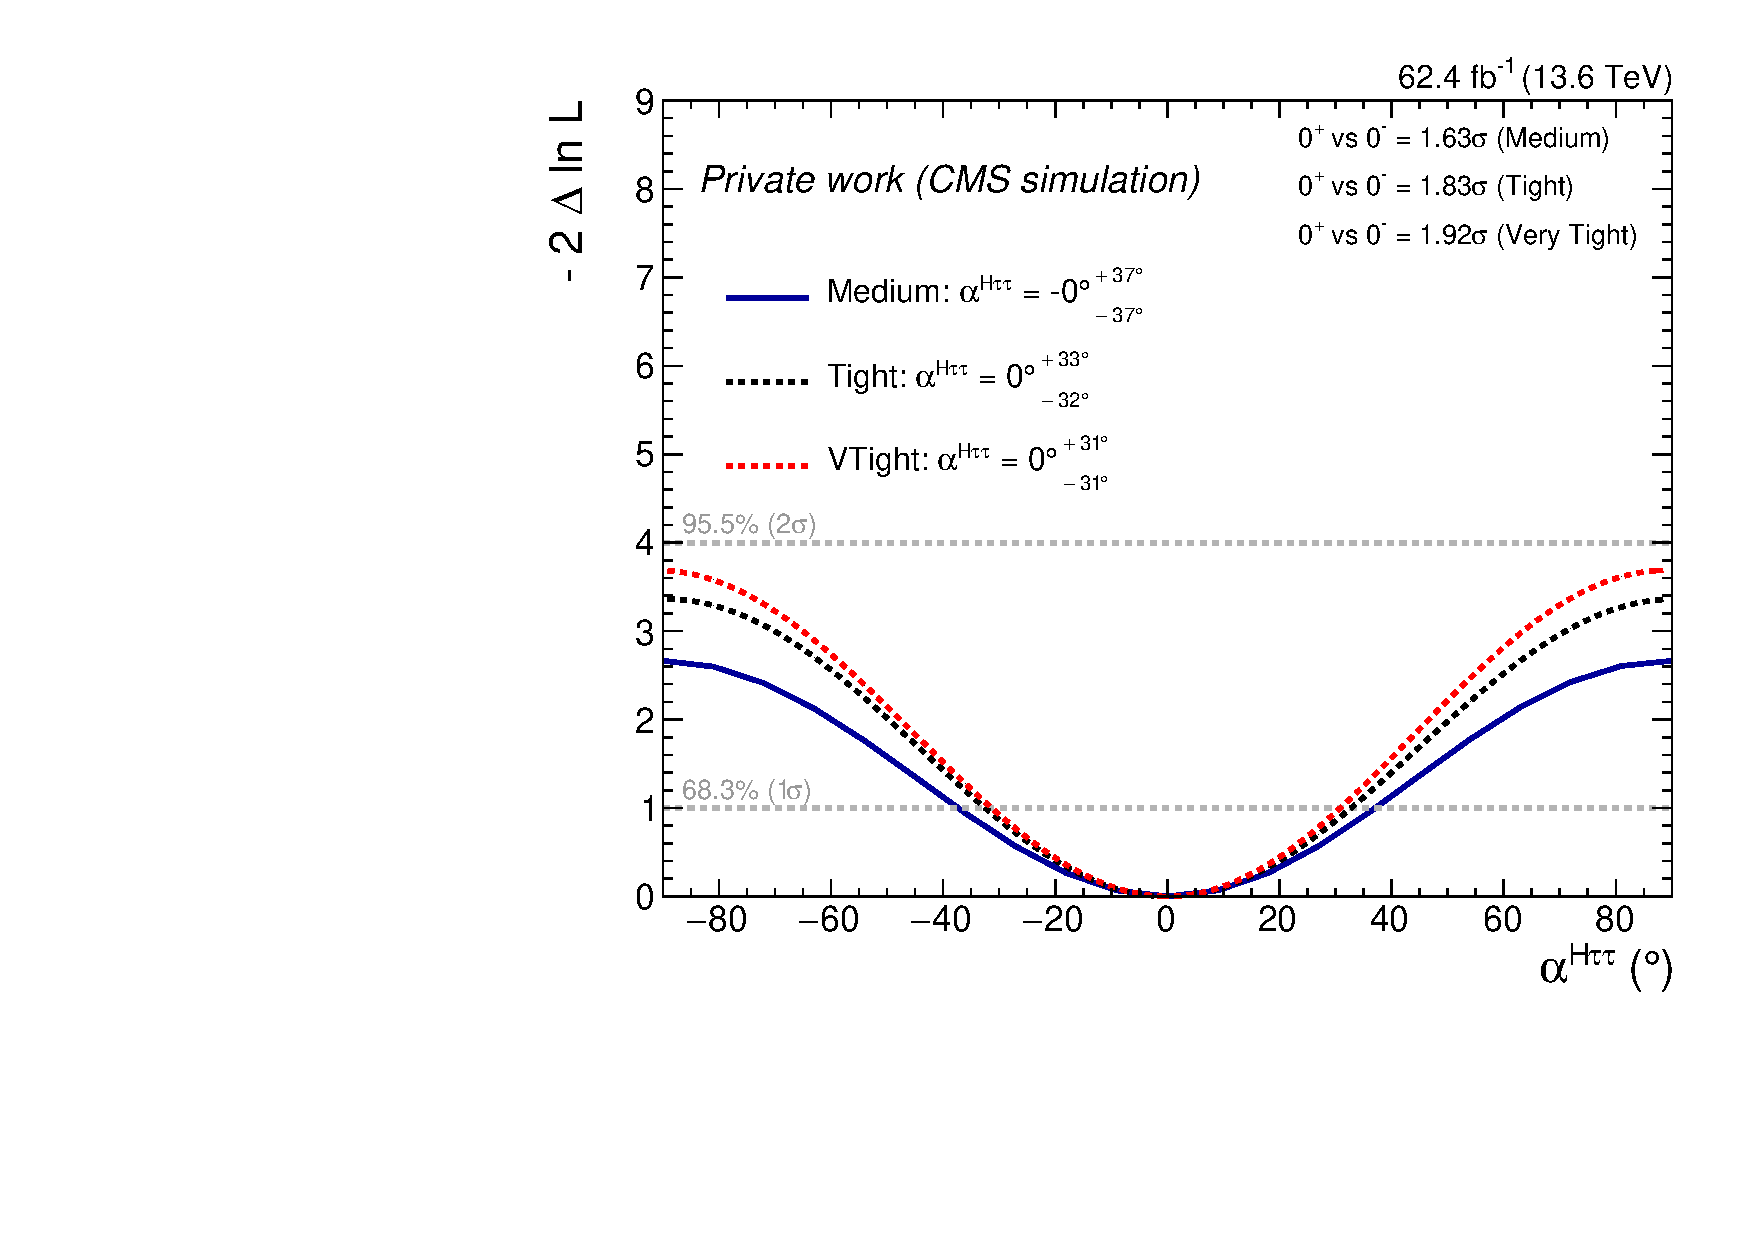
\includegraphics[width=0.8\textwidth]{Figures/Chapter7/alpha/alpha_WP.pdf}
    \caption[Expected sensitivity scan for different $D_{\text{jet}}$ working points.]
    {Expected exclusion sensitivity of the pure CP-odd scenario for three $D_{\text{jet}}$ working points (Medium, Tight, and VTight). The sensitivities shown here differ slightly from those in Tables~\ref{Table:Chapter7_IPsignificance_Optimisation}-~\ref{Table:Chapter7_yrho_Optimisation}, as the figure includes the impact of nuisance parameters, which are not considered in the table results. The overall conclusions, however, remain unchanged.}
    \label{Figure:Chapter7_WP_Optimisation}
\end{figure}

\section{Results}

Building on the methodology and analysis framework established in the previous sections, this section presents the results of this analysis. The discussion begins with postfit distributions of the relevant observables, followed by likelihood scans of the CP-sensitive variable. The sensitivity achieved in each category is then compared to that of the precursor analysis~\cite{HiggsCP_CMS_2021}, highlighting the gains from the current strategy. Finally, the outcome of the statistical combination of this analysis with its predecessor is presented.

\subsection{Postfit distributions}

Postfit distributions are presented following the simultaneous fit to the data, performed across all categories of the analysis. The background contributions are split into three groups, in accordance with the definitions introduced in Section~\ref{Section:Chapter7_Background_Modelling}:

\begin{enumerate}
    \item \textbf{Genuine $\tauh$ leptons:} Events with two genuine $\tauh$ candidates, dominated by the \ac{DY} process.
    \item \textbf{Jet$\to \tauh$:} Events containing one or more jets misidentified as $\tauh$ candidates.
    \item \textbf{Others:} Contributions from processes such as $\ttbar$, single-top, diboson, and \ac{DY}, in which one $\tauh$ candidate is genuine and the other is a misidentified lepton, or in which both $\tauh$ candidates are misidentified leptons.
\end{enumerate}

In addition, the $H\to\tau\tau$ signal is shown, with contributions from \ac{ggH}, \ac{VBF}, and \ac{VH}.

Postfit distributions of the BDT score in the Genuine and Mis-identified (Mis-ID) categories are shown first in Fig.~\ref{Figure:Chapter7_Postfit_BDT}. As expected, events from the genuine ditau and jet\textrightarrow$\tauh$ backgrounds populate high BDT scores in the Genuine and Mis-ID categories, respectively. This demonstrates the effectiveness of the \ac{BDT} classifier in separating the dominant background types. The data and simulated expectations agree within uncertainties. While these distributions do not carry direct sensitivity to the CP structure of the Higgs boson coupling, their inclusion in the fit is crucial for constraining background normalisations and associated uncertainties. Signal templates corresponding to a purely CP-odd ($\mathrm{PS}$) coupling and to the best-fit result are overlaid for comparison.

\begin{figure}[!htbp]
        \centering
        % First row
        \begin{subfigure}[b]{0.7\textwidth}
            \centering
            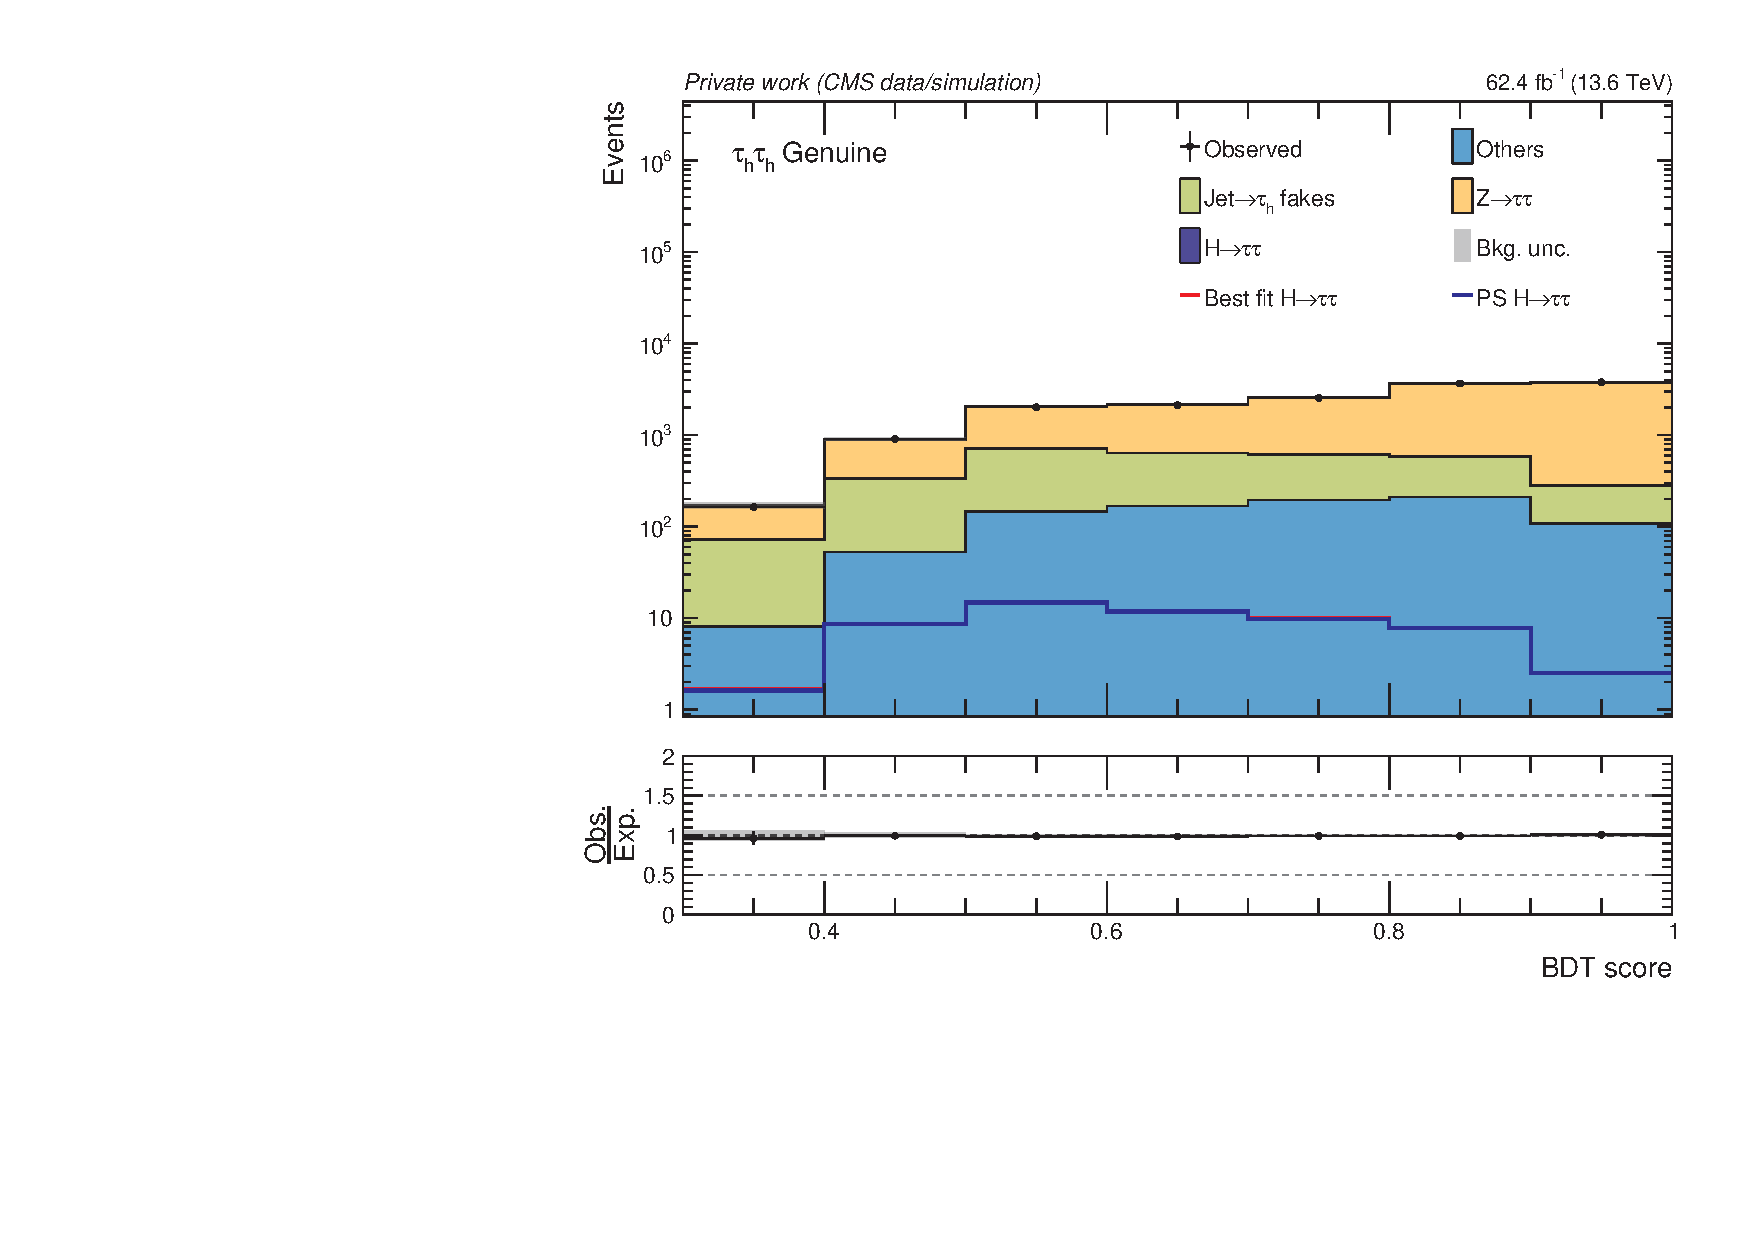
\includegraphics[width=\textwidth]{Figures/Chapter7/postfit/htt_tt_1_13p6TeV.pdf}
            \caption{}
        \end{subfigure}
        \begin{subfigure}[b]{0.7\textwidth}
            \centering
            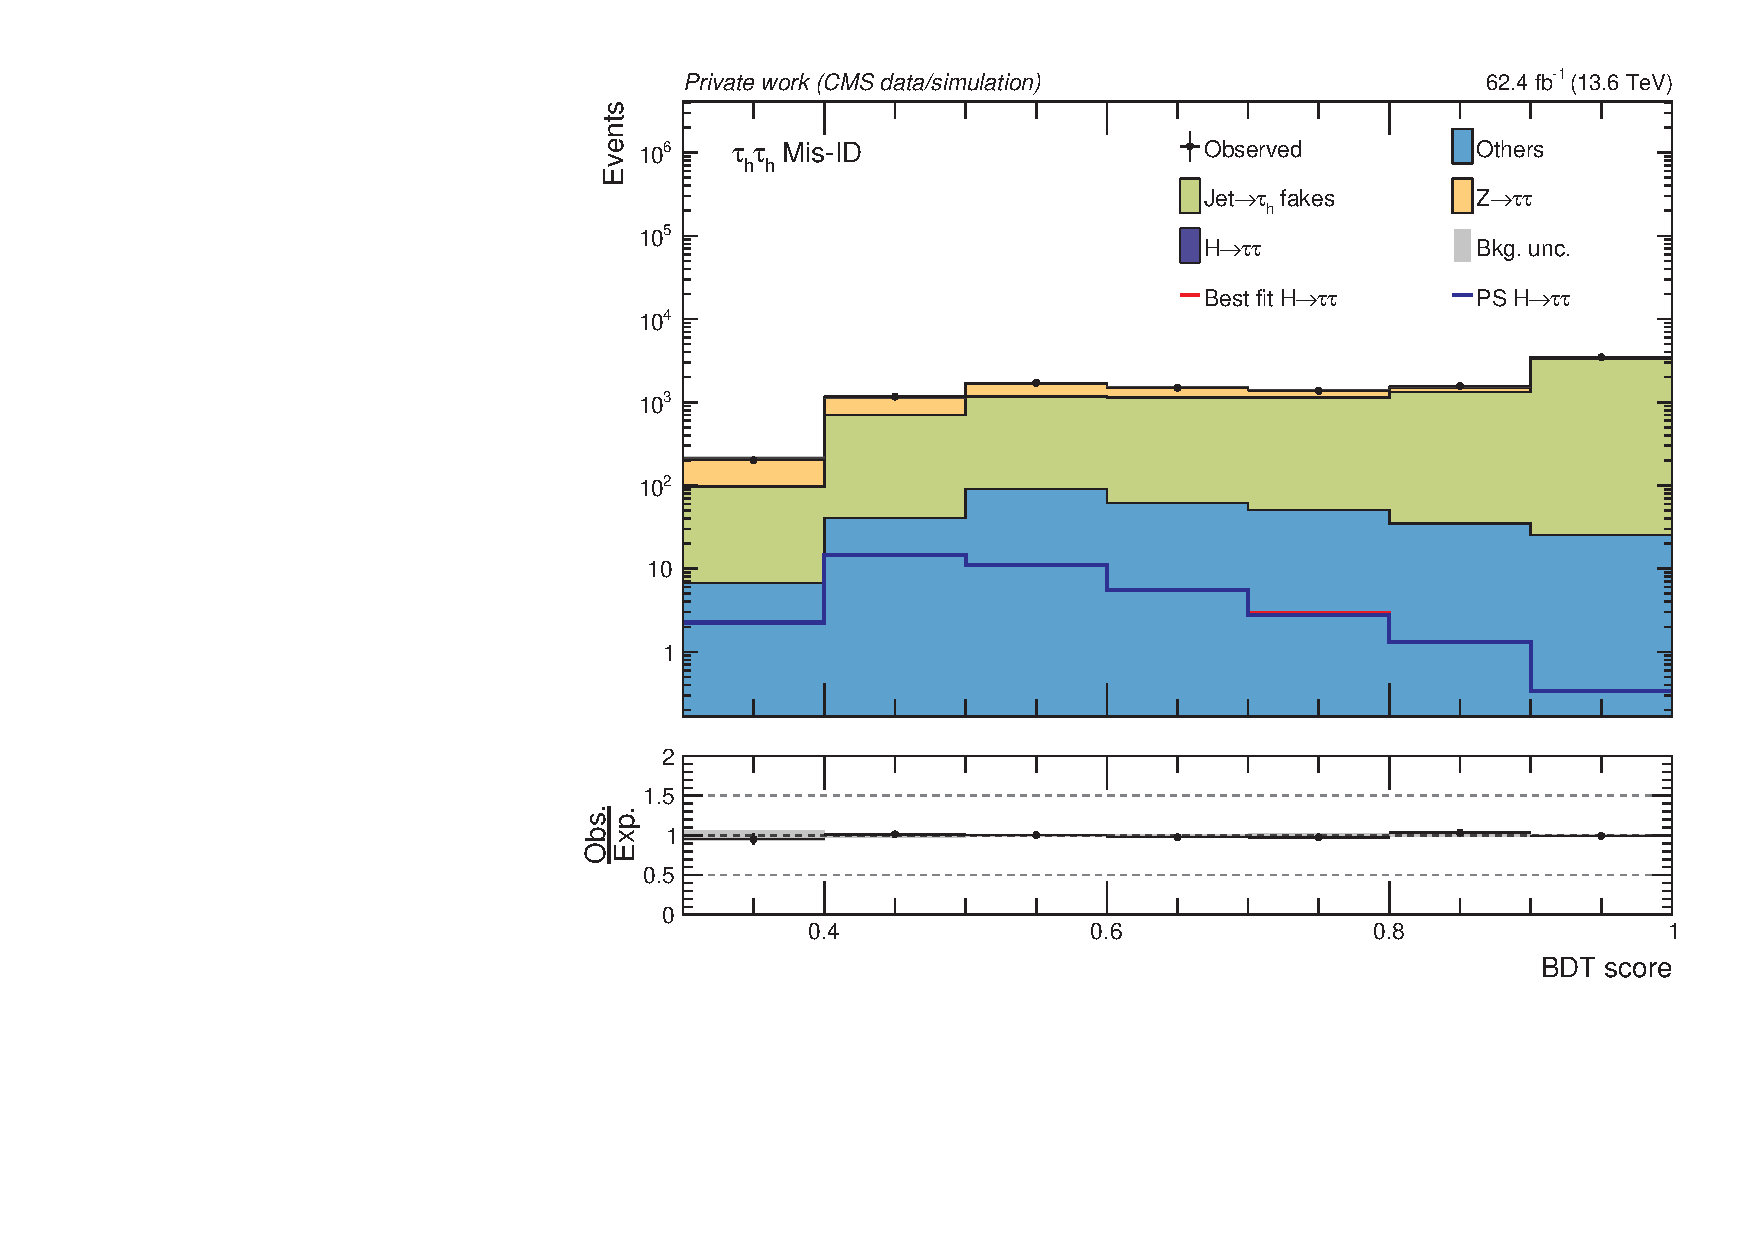
\includegraphics[width=\textwidth]{Figures/Chapter7/postfit/htt_tt_2_13p6TeV.pdf}
            \caption{}
        \end{subfigure}
    \caption{Postfit BDT score distributions in the \textbf{(a)} Genuine $\tau_h$ and \textbf{(b)} Mis-ID categories.}
    \label{Figure:Chapter7_Postfit_BDT}
\end{figure}

Subsequently, the unrolled two-dimensional discriminants are shown after the fit. In these figures, the binning of the acoplanarity angle, defined in the range $[0,2\pi]$, is indicated along the horizontal axis, while the binning of the BDT score is displayed through the broken vertical lines, with labels indicating the corresponding intervals. These distributions, shown in Fig.~\ref{Figure:Chapter7_Postfit_Unrolled_1}--\ref{Figure:Chapter7_Postfit_Unrolled_9}, highlight the ability of the analysis to separate signal from background, with the \ac{BDT} effectively assigning large scores to signal-like events and low scores to background-dominated regions.

\begin{figure}[!htbp]
    \centering
    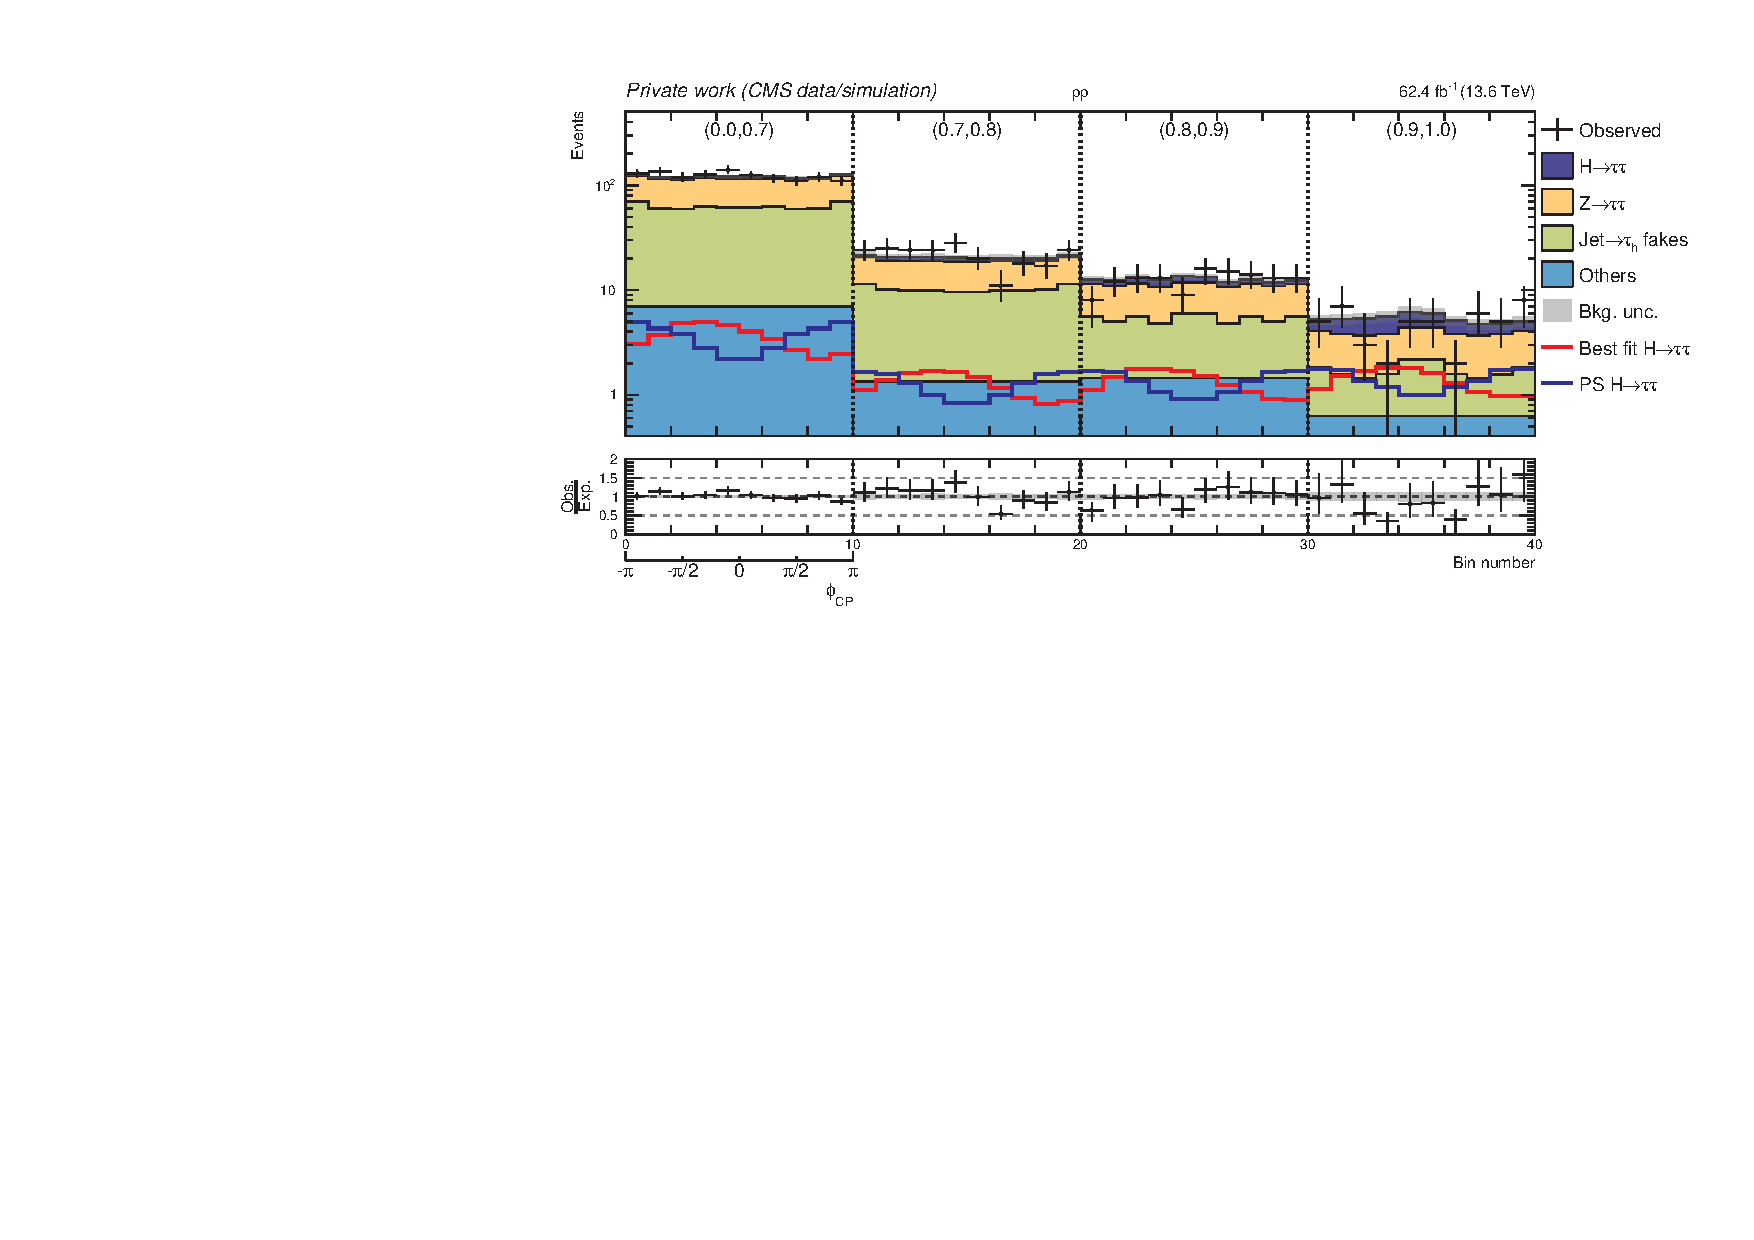
\includegraphics[width=1\textwidth]{Figures/Chapter7/postfit/htt_tt_3_13p6TeV.pdf}
    \caption[Postfit $\phi_{CP}$ distribution in the $\rho\rho$ category.]
    {Postfit $\phi_{CP}$ distribution in the $\rho\rho$ category, shown in bins of \ac{BDT} score. Overlaid are the signal distributions for a purely CP-odd coupling and for the best-fit result. The binning of the BDT score is displayed through the broken vertical lines, with labels indicating the corresponding intervals.}
    \label{Figure:Chapter7_Postfit_Unrolled_1}
\end{figure}

\begin{figure}[!htbp]
    \centering
    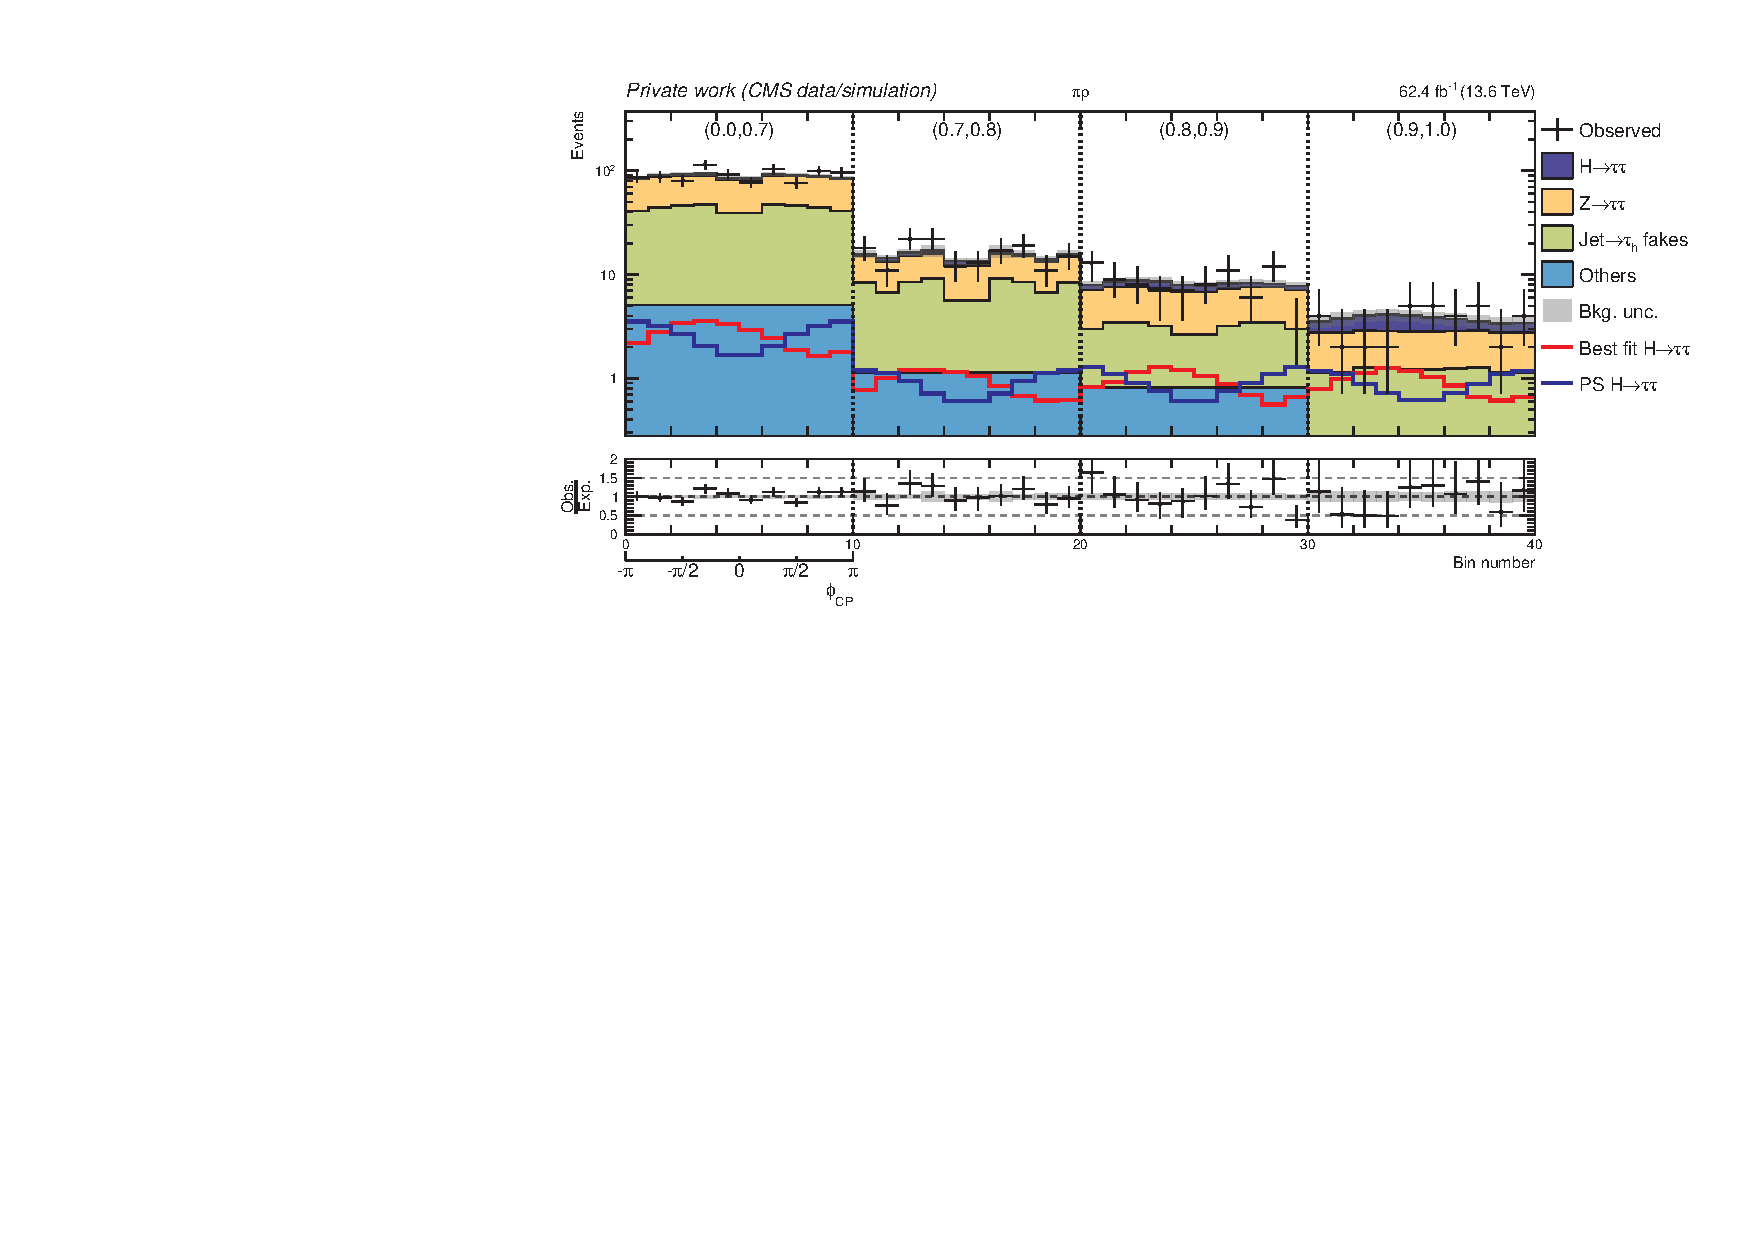
\includegraphics[width=1\textwidth]{Figures/Chapter7/postfit/htt_tt_7_13p6TeV.pdf}
    \caption[Postfit $\phi_{CP}$ distribution in the $\pi\rho$ category.]
    {Postfit $\phi_{CP}$ distribution in the $\pi\rho$ category, shown in bins of \ac{BDT} score. Overlaid are the signal distributions for a purely CP-odd coupling and for the best-fit result. The binning of the BDT score is displayed through the broken vertical lines, with labels indicating the corresponding intervals.}
    \label{Figure:Chapter7_Postfit_Unrolled_2}
\end{figure}

\begin{figure}[!htbp]
    \centering
    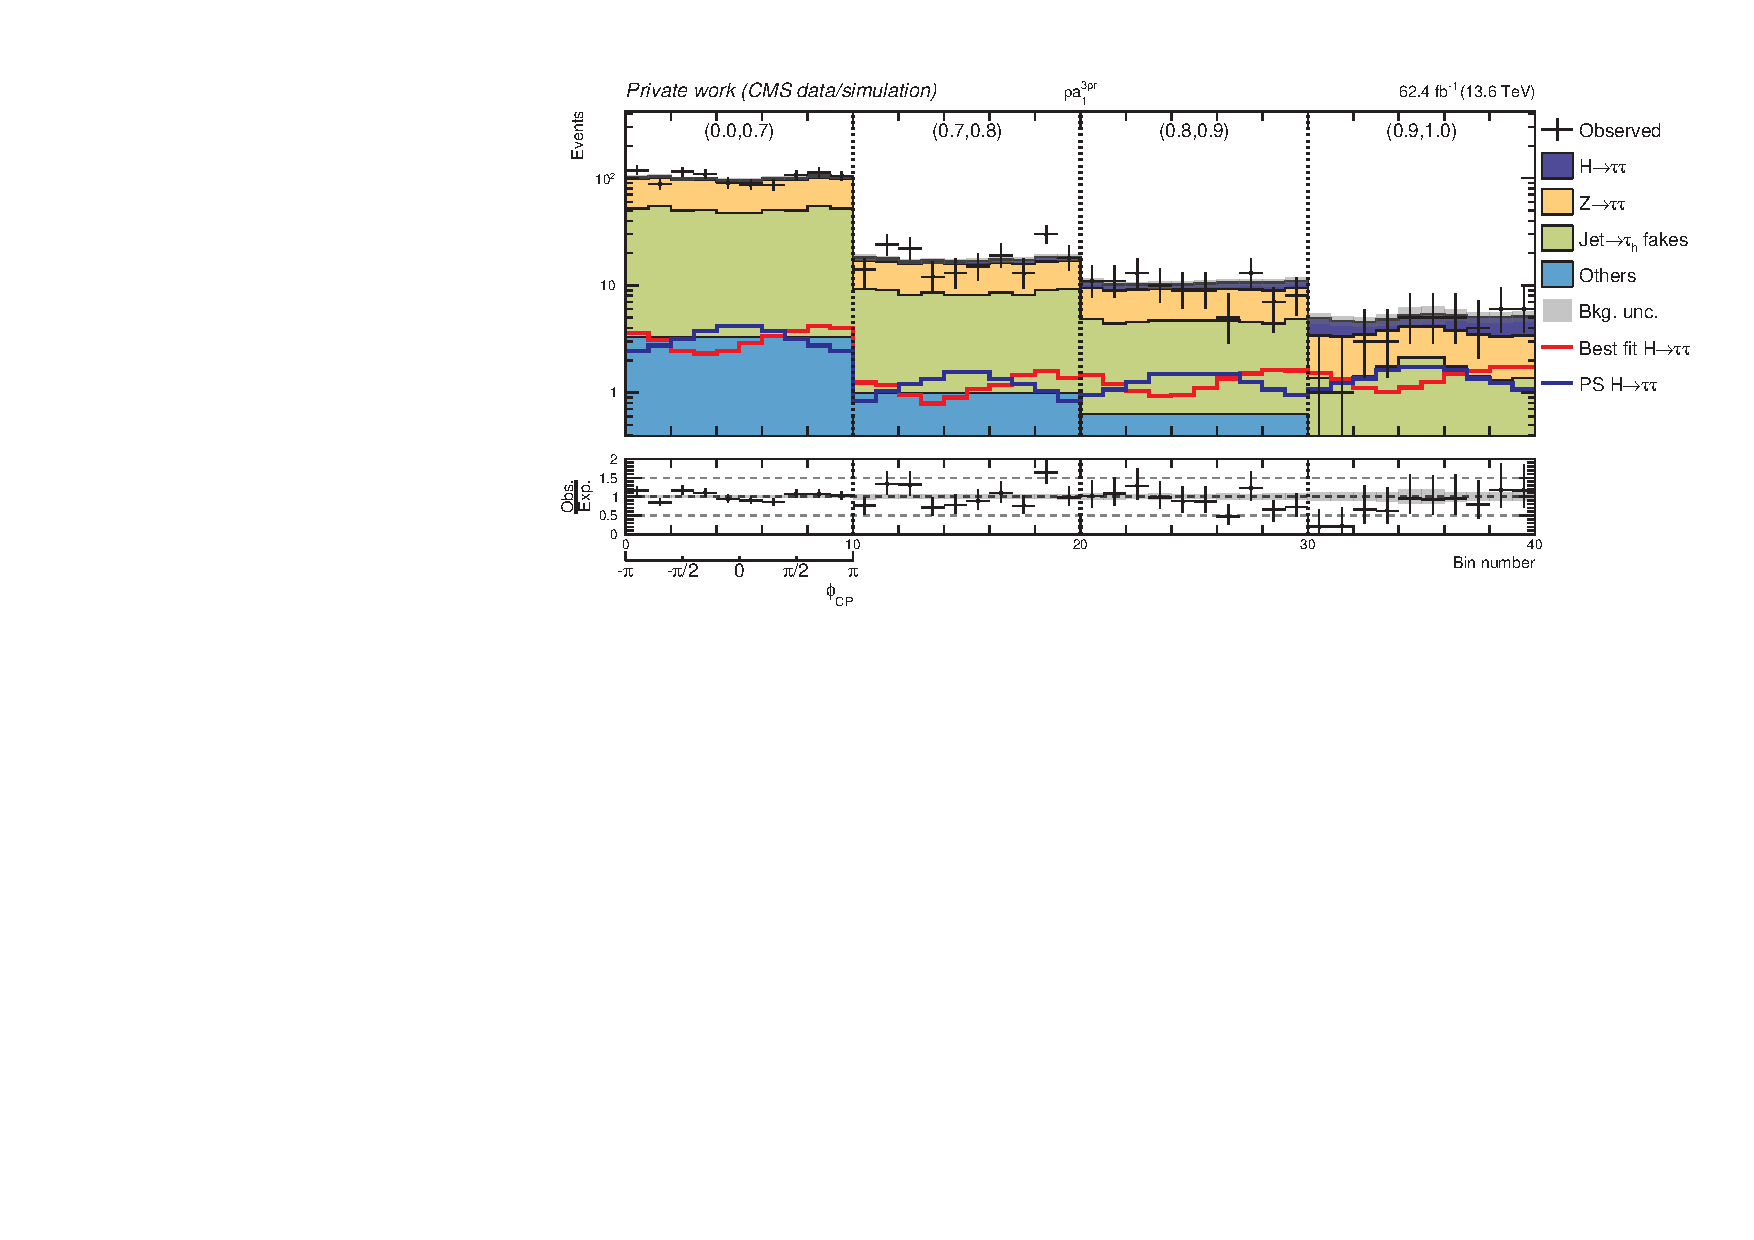
\includegraphics[width=1\textwidth]{Figures/Chapter7/postfit/htt_tt_5_13p6TeV.pdf}
    \caption[Postfit $\phi_{CP}$ distribution in the $\rho a_1^\text{3pr}$ category.]
    {Postfit $\phi_{CP}$ distribution in the $\rho a_1^\text{3pr}$ category, shown in bins of \ac{BDT} score. Overlaid are the signal distributions for a purely CP-odd coupling and for the best-fit result. The binning of the BDT score is displayed through the broken vertical lines, with labels indicating the corresponding intervals.}
    \label{Figure:Chapter7_Postfit_Unrolled_3}
\end{figure}

\begin{figure}[!htbp]
    \centering
    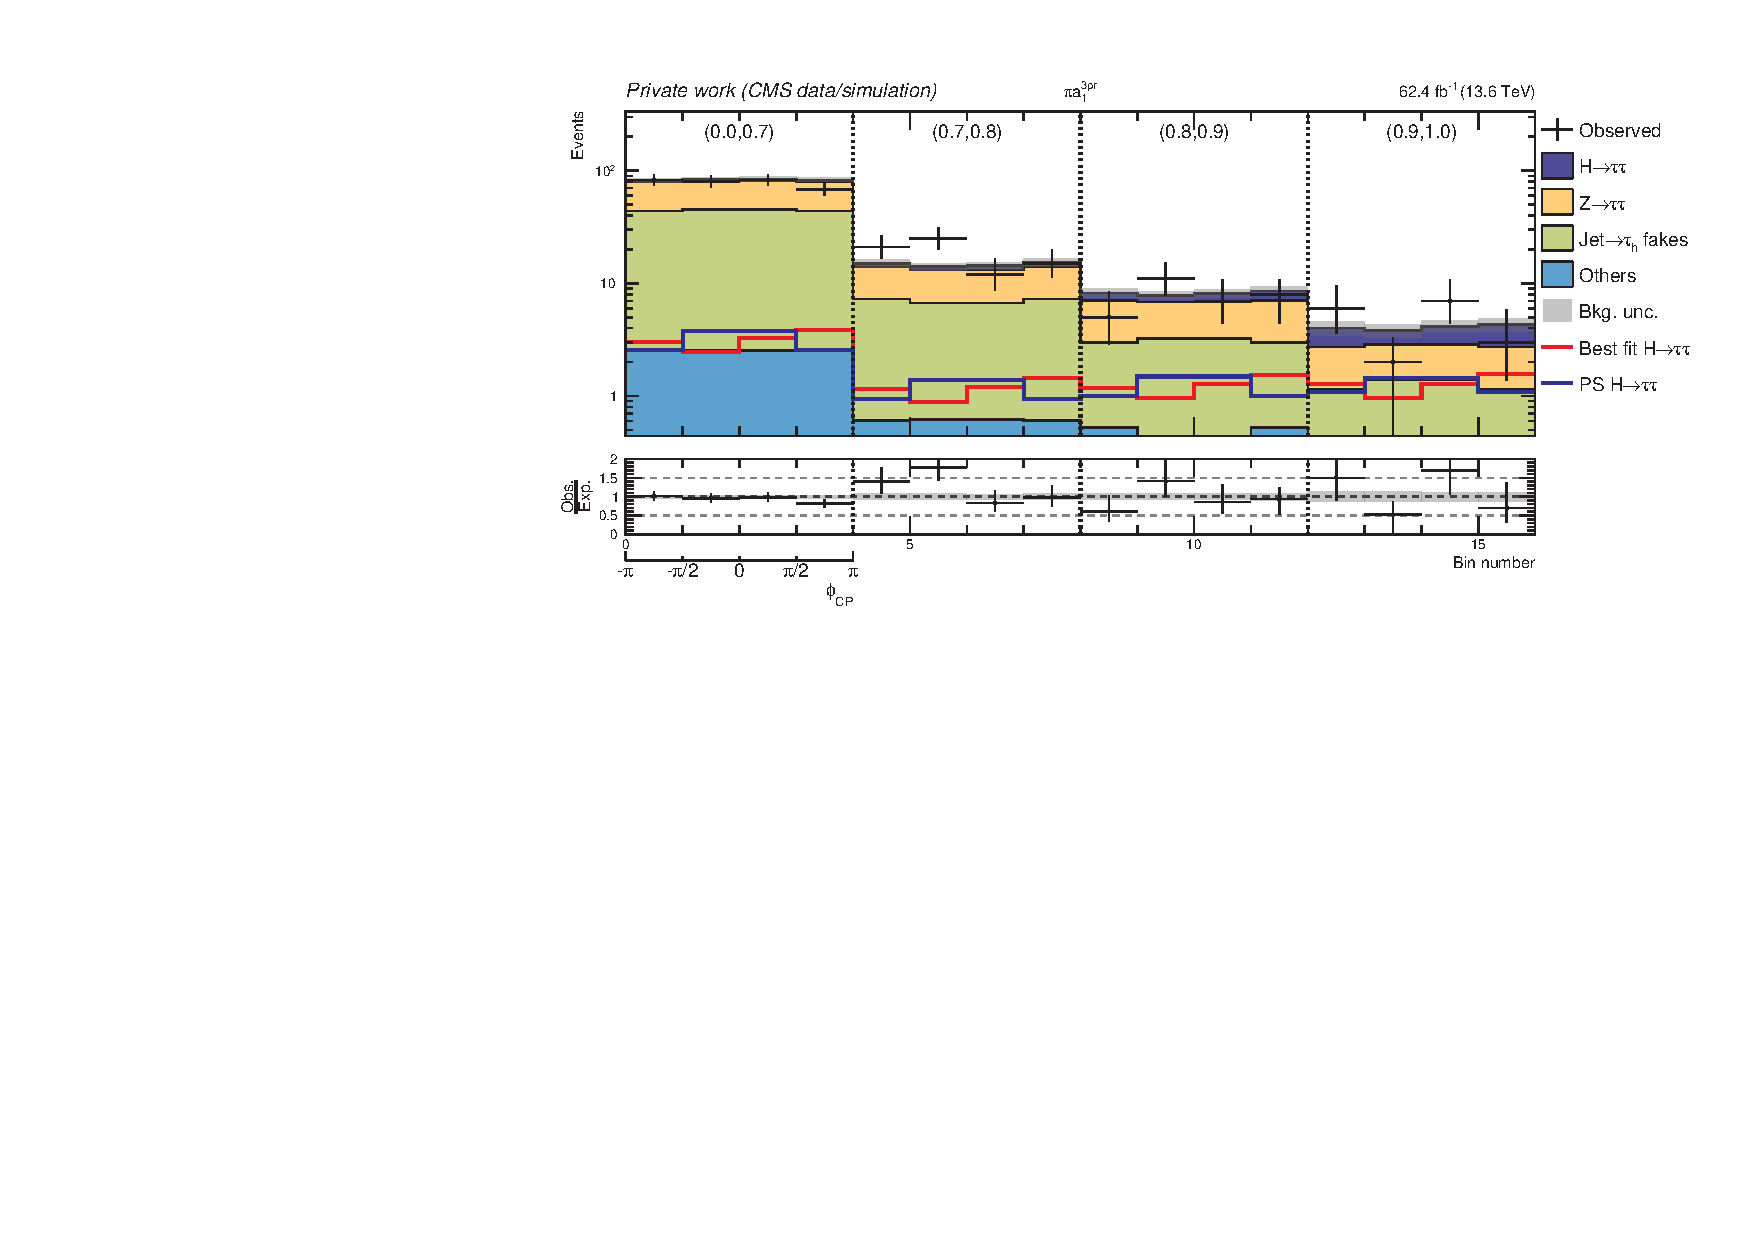
\includegraphics[width=1\textwidth]{Figures/Chapter7/postfit/htt_tt_9_13p6TeV.pdf}
    \caption[Postfit $\phi_{CP}$ distribution in the $\pi a_1^\text{3pr}$ category.]
    {Postfit $\phi_{CP}$ distribution in the $\pi a_1^\text{3pr}$ category, shown in bins of \ac{BDT} score. Overlaid are the signal distributions for a purely CP-odd coupling and for the best-fit result. The binning of the BDT score is displayed through the broken vertical lines, with labels indicating the corresponding intervals.}
    \label{Figure:Chapter7_Postfit_Unrolled_4}
\end{figure}

\begin{figure}[!htbp]
    \centering
    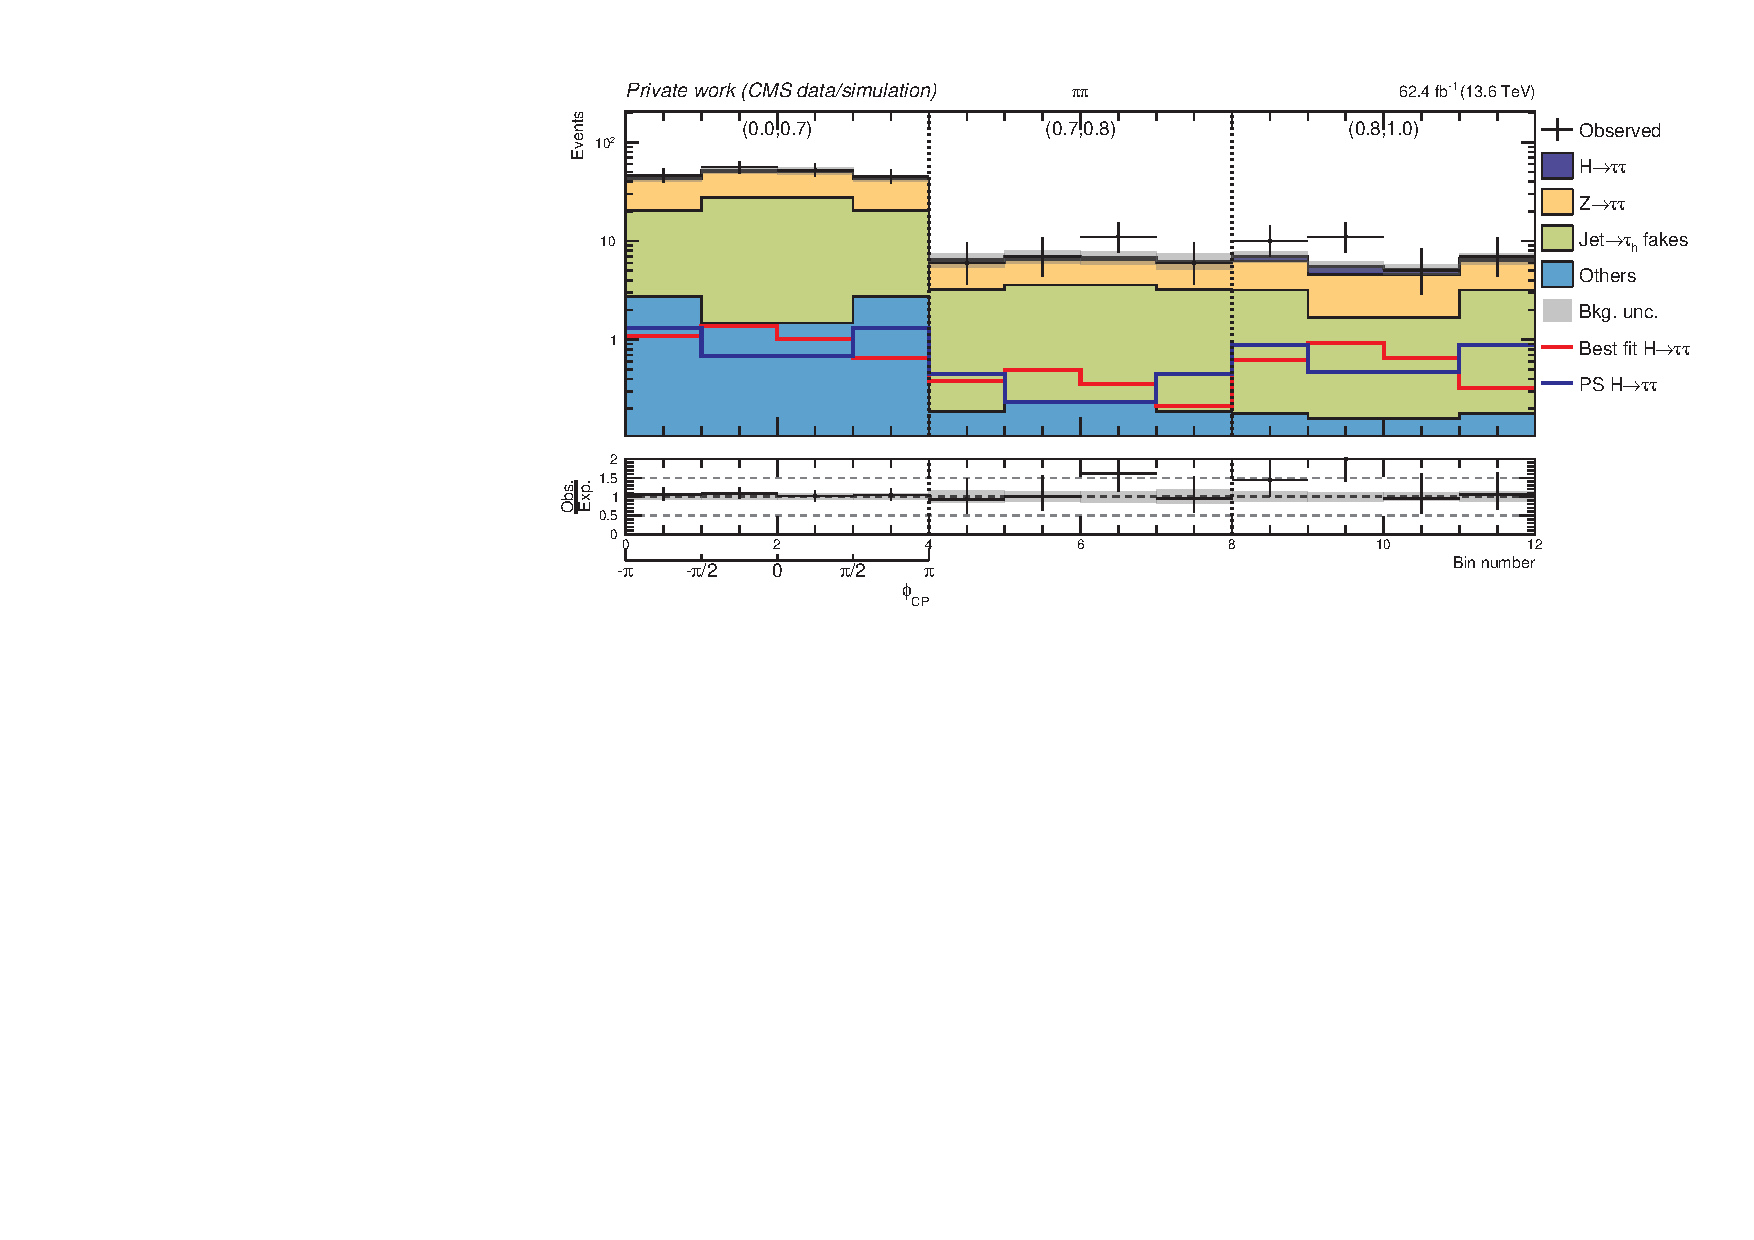
\includegraphics[width=1\textwidth]{Figures/Chapter7/postfit/htt_tt_8_13p6TeV.pdf}
    \caption[Postfit $\phi_{CP}$ distribution in the $\pi \pi$ category.]
    {Postfit $\phi_{CP}$ distribution in the $\pi \pi$ category, shown in bins of \ac{BDT} score. Overlaid are the signal distributions for a purely CP-odd coupling and for the best-fit result. The binning of the BDT score is displayed through the broken vertical lines, with labels indicating the corresponding intervals.}
    \label{Figure:Chapter7_Postfit_Unrolled_5}
\end{figure}

\begin{figure}[!htbp]
    \centering
    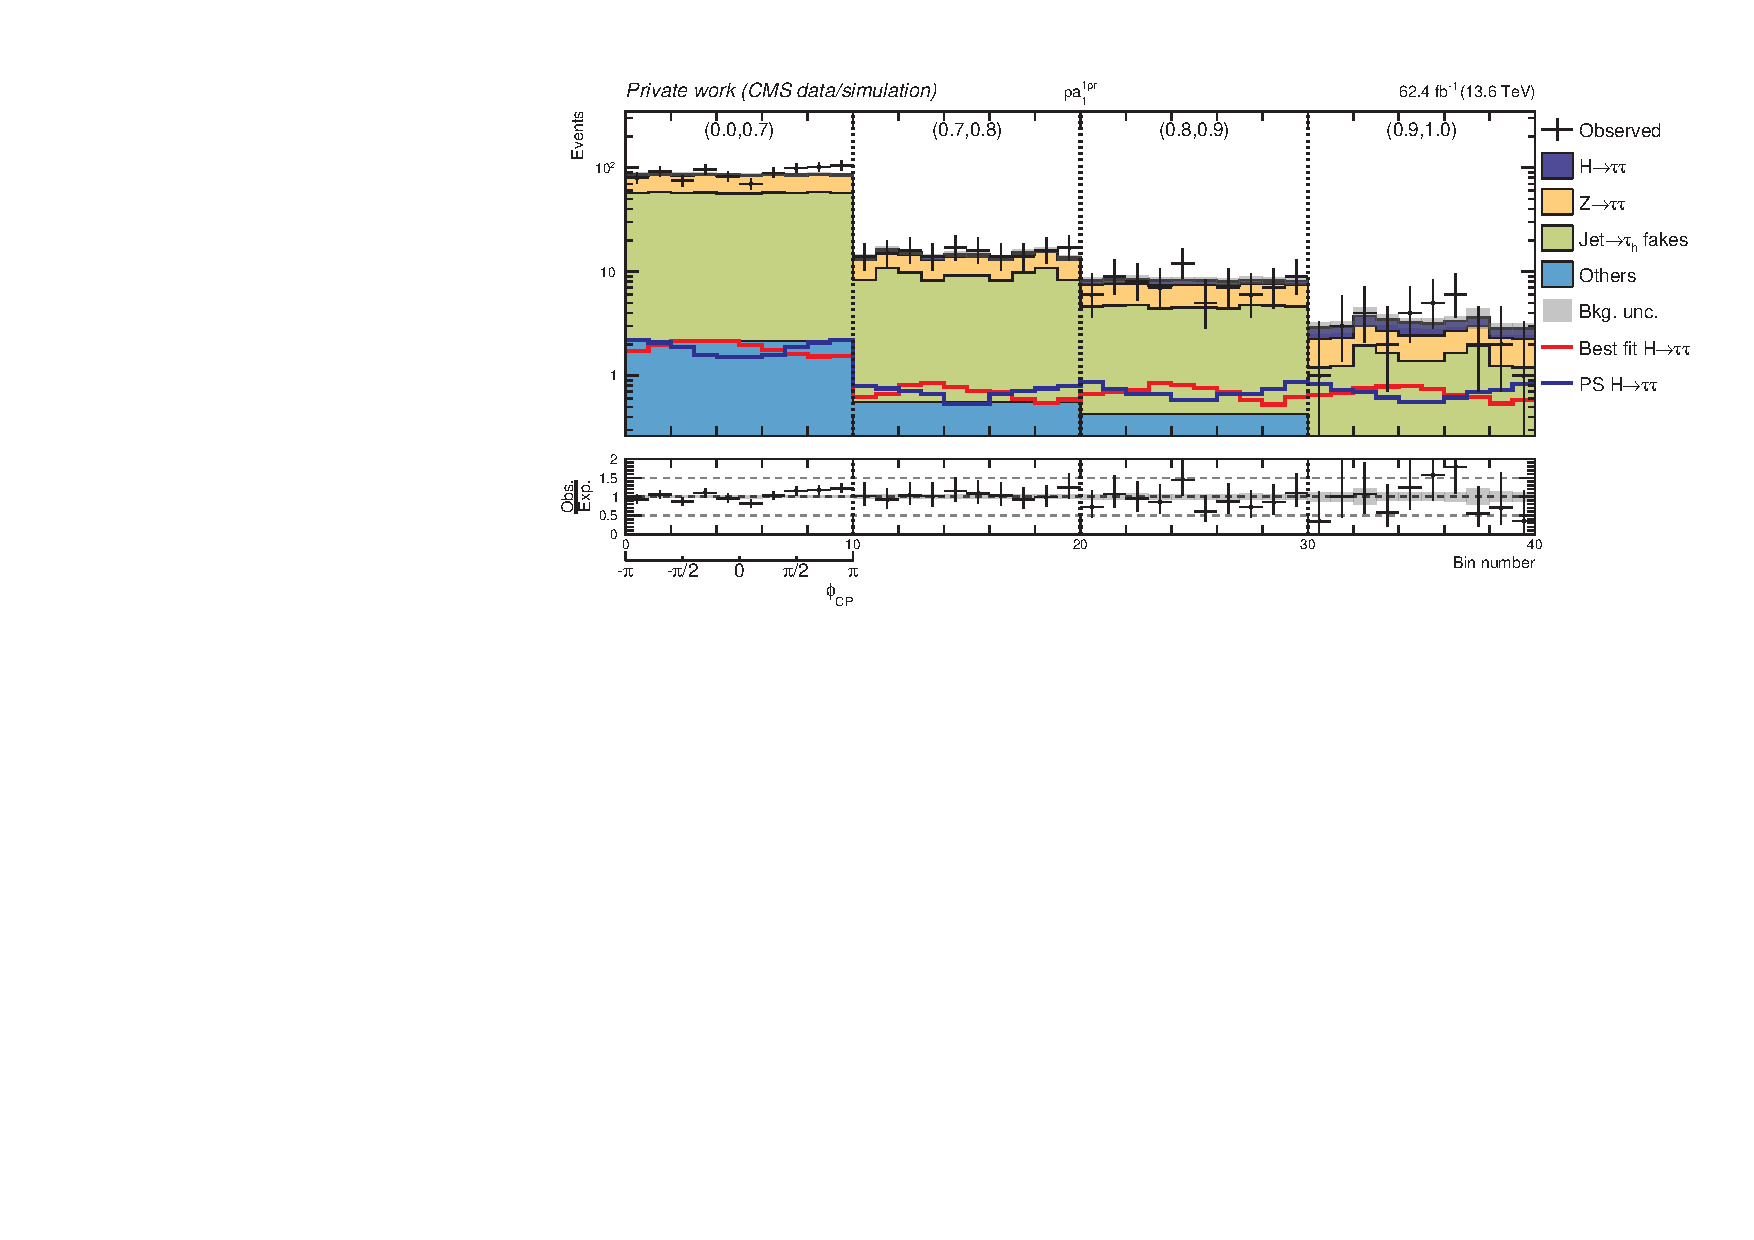
\includegraphics[width=1\textwidth]{Figures/Chapter7/postfit/htt_tt_4_13p6TeV.pdf}
    \caption[Postfit $\phi_{CP}$ distribution in the $a_1^\text{1pr}\rho + a_1^\text{1pr}a_1^\text{1pr}$ category.]
    {Postfit $\phi_{CP}$ distribution in the $a_1^\text{1pr}\rho + a_1^\text{1pr}a_1^\text{1pr}$ category, shown in bins of \ac{BDT} score. Overlaid are the signal distributions for a purely CP-odd coupling and for the best-fit result. The binning of the BDT score is displayed through the broken vertical lines, with labels indicating the corresponding intervals.}
    \label{Figure:Chapter7_Postfit_Unrolled_6}
\end{figure}

\begin{figure}[!htbp]
    \centering
    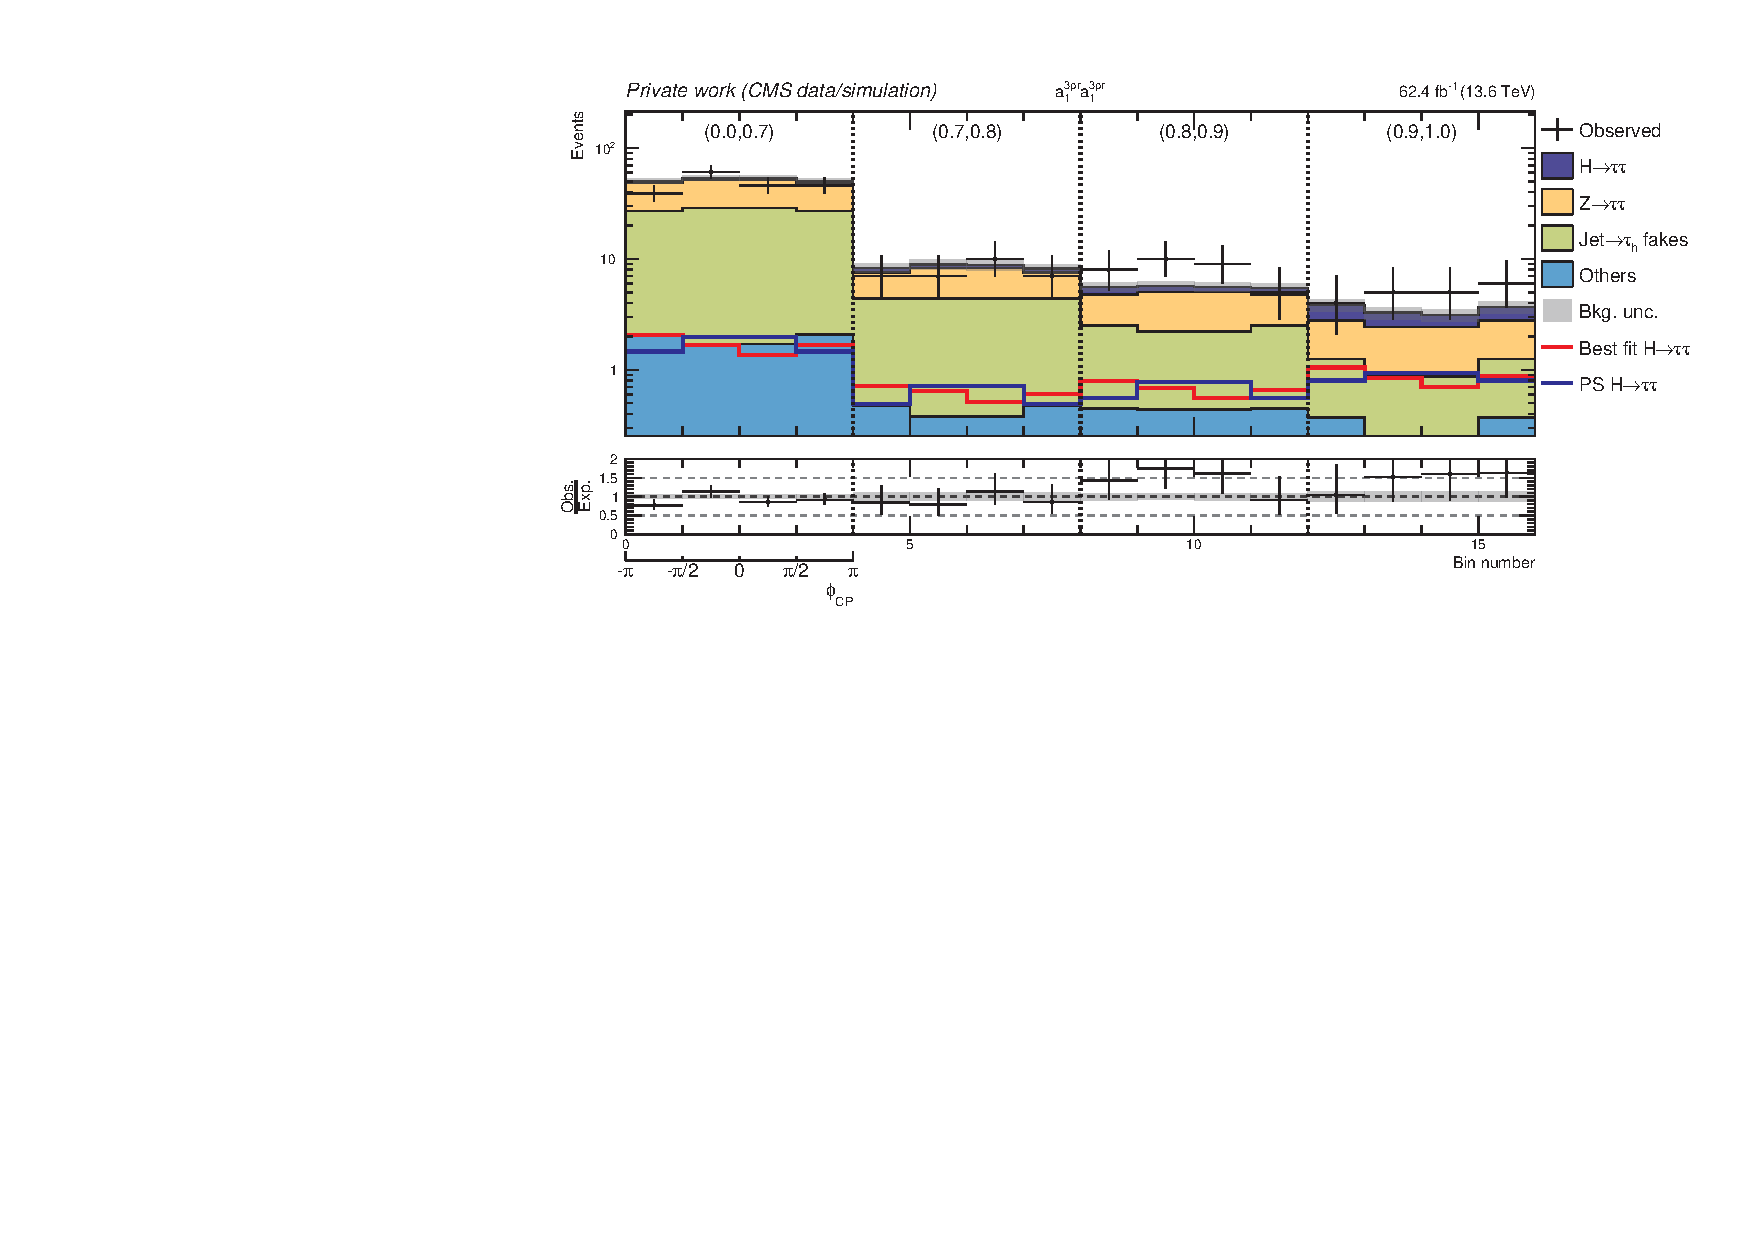
\includegraphics[width=1\textwidth]{Figures/Chapter7/postfit/htt_tt_6_13p6TeV.pdf}
    \caption[Postfit $\phi_{CP}$ distribution in the $a_1^\text{3pr}a_1^\text{3pr}$ category.]
    {Postfit $\phi_{CP}$ distribution in the $a_1^\text{3pr}a_1^\text{3pr}$ category, shown in bins of \ac{BDT} score. Overlaid are the signal distributions for a purely CP-odd coupling and for the best-fit result. The binning of the BDT score is displayed through the broken vertical lines, with labels indicating the corresponding intervals.}
    \label{Figure:Chapter7_Postfit_Unrolled_7}
\end{figure}

\begin{figure}[!htbp]
    \centering
    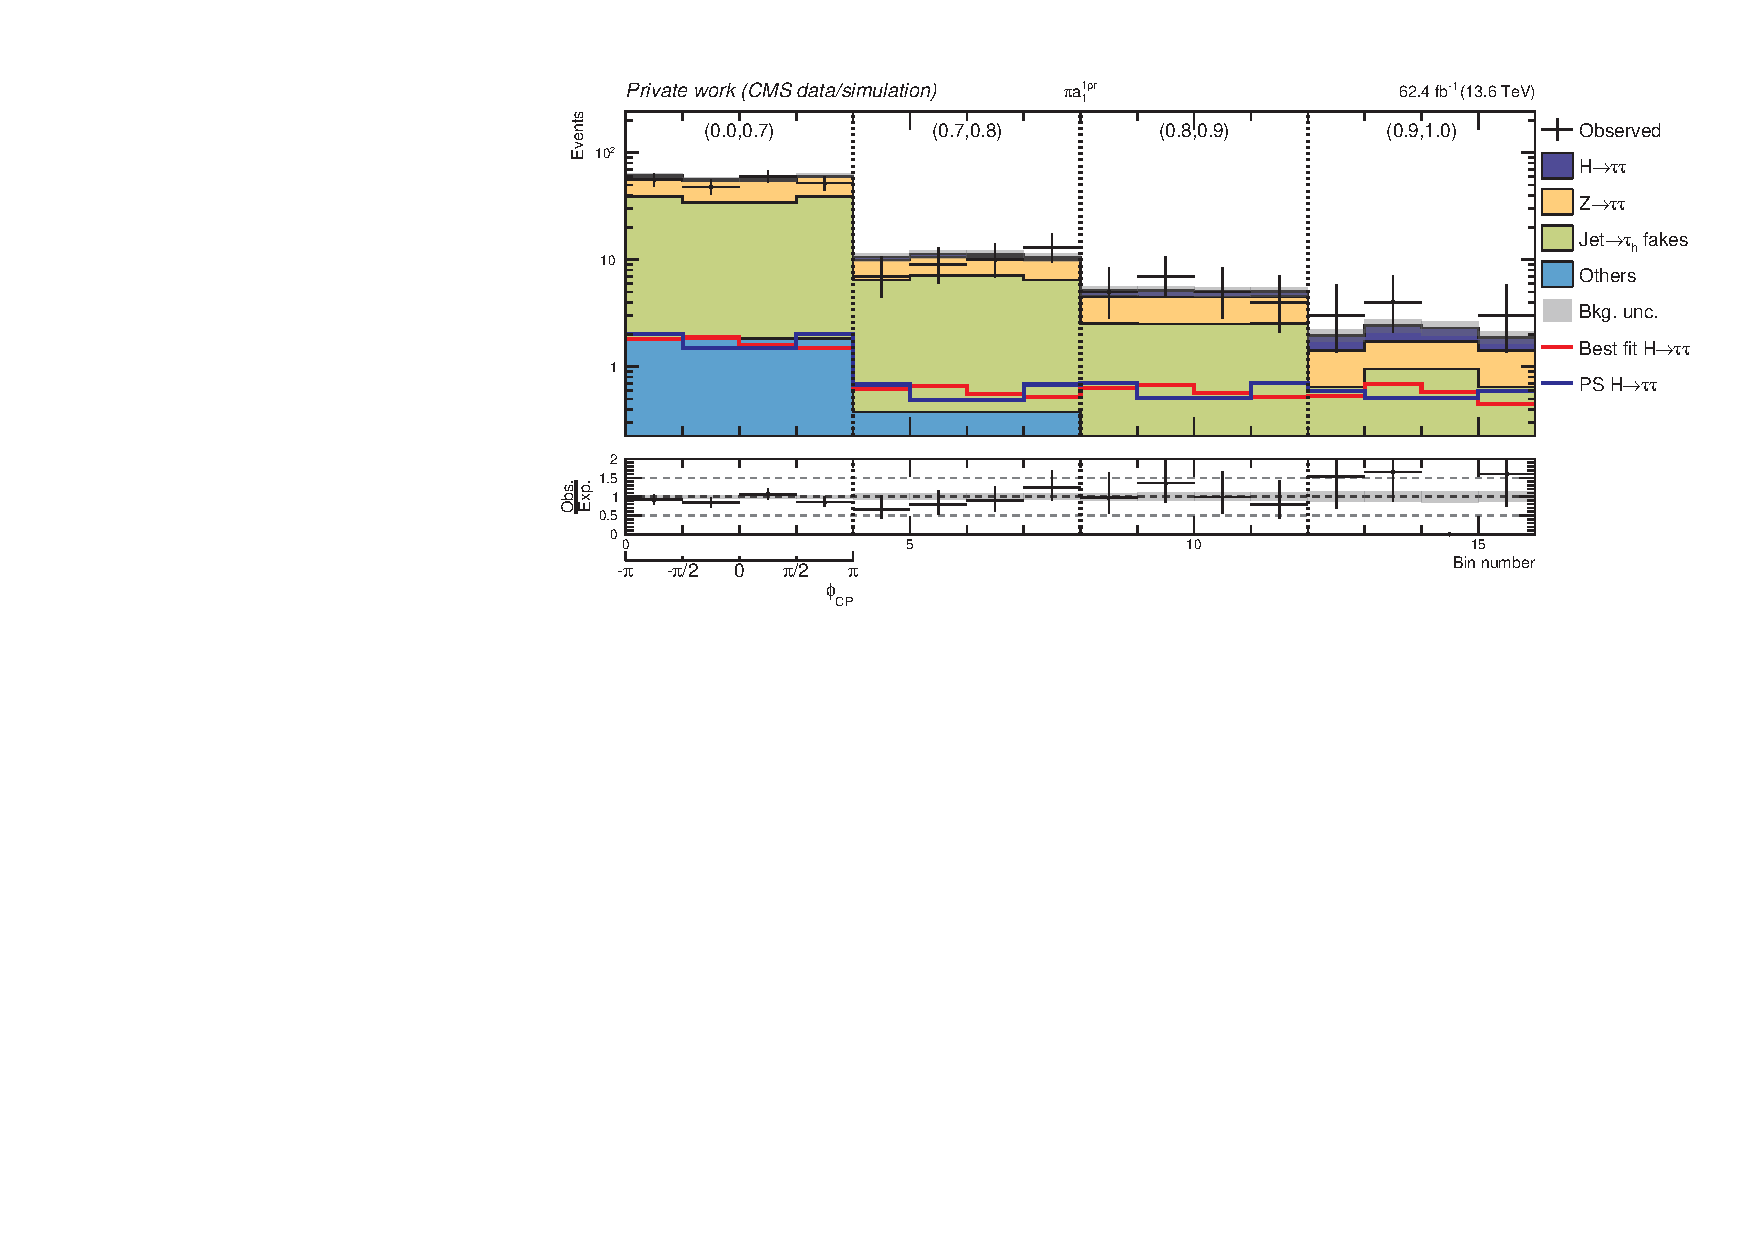
\includegraphics[width=1\textwidth]{Figures/Chapter7/postfit/htt_tt_10_13p6TeV.pdf}
    \caption[Postfit $\phi_{CP}$ distribution in the $\pi a_1^\text{1pr}$ category.]
    {Postfit $\phi_{CP}$ distribution in the $\pi a_1^\text{1pr}$ category, shown in bins of \ac{BDT} score. Overlaid are the signal distributions for a purely CP-odd coupling and for the best-fit result. The binning of the BDT score is displayed through the broken vertical lines, with labels indicating the corresponding intervals.}
    \label{Figure:Chapter7_Postfit_Unrolled_8}
\end{figure}

\begin{figure}[!htbp]
    \centering
    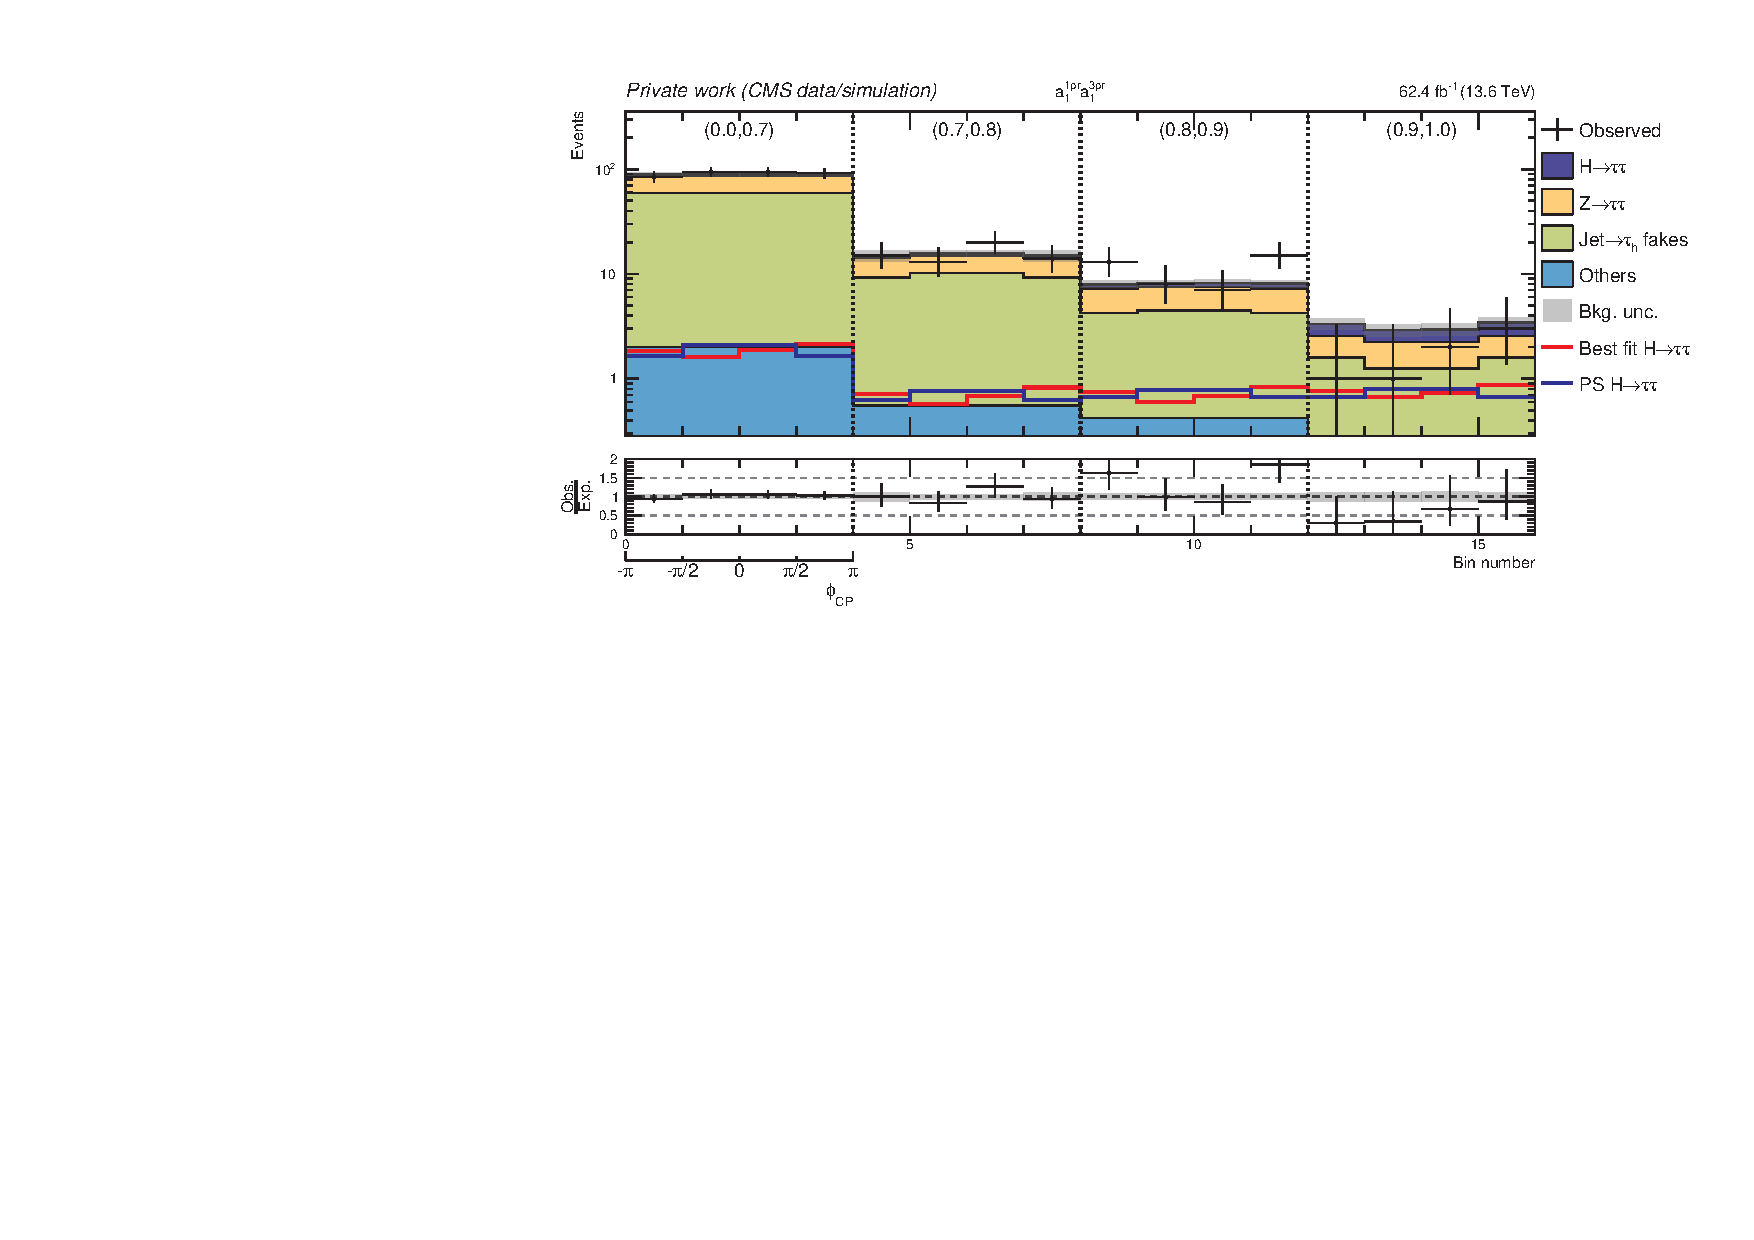
\includegraphics[width=1\textwidth]{Figures/Chapter7/postfit/htt_tt_11_13p6TeV.pdf}
    \caption[Postfit $\phi_{CP}$ distribution in the $a_1^\text{1pr}a_1^\text{3pr}$ category.]
    {Postfit $\phi_{CP}$ distribution in the $a_1^\text{1pr}a_1^\text{3pr}$ category, shown in bins of \ac{BDT} score. Overlaid are the signal distributions for a purely CP-odd coupling and for the best-fit result. The binning of the BDT score is displayed through the broken vertical lines, with labels indicating the corresponding intervals.}
    \label{Figure:Chapter7_Postfit_Unrolled_9}
\end{figure}

\subsection{\texorpdfstring{$\alpha^{\PH\tau\tau}$}{alphatautau} mixing angle}

The observed and expected negative log-likelihood scans for the combination of all analysis categories in the $\tauh\tauh$ final state are shown in Fig.~\ref{Figure:Chapter7_LLScan}. As discussed in Section~\ref{Section:Chapter7_StatisticalProcedure}, a freely-floating single rate parameter scaling the overall signal strength is used. The best fit value of this parameter is $\mu_{\tau\tau}= 0.94 \pm 0.33$.

The data disfavour the pure CP-odd scenario at \textbf{1.74$\sigma$}, compared to an expected exclusion of \textbf{2.39$\sigma$}. The observed sensitivity to the $\alpha^{\PH\tau\tau}$ mixing angle is weaker than the expectation, which can be attributed to statistical fluctuations in the data. In particular, the sensitivity of the $\phi_{CP}$ observable relies strongly on the amplitude and phase of the modulation. Such statistical fluctuations could distort the observed $\phi_{CP}$ shape. When these fluctuations generate a modulation pattern inconsistent with both the CP-even and CP-odd templates, the fit compensates by broadening the likelihood scan, which manifests as an increased uncertainty in the determination of the mixing angle.

\begin{figure}[!htbp]
    \centering
    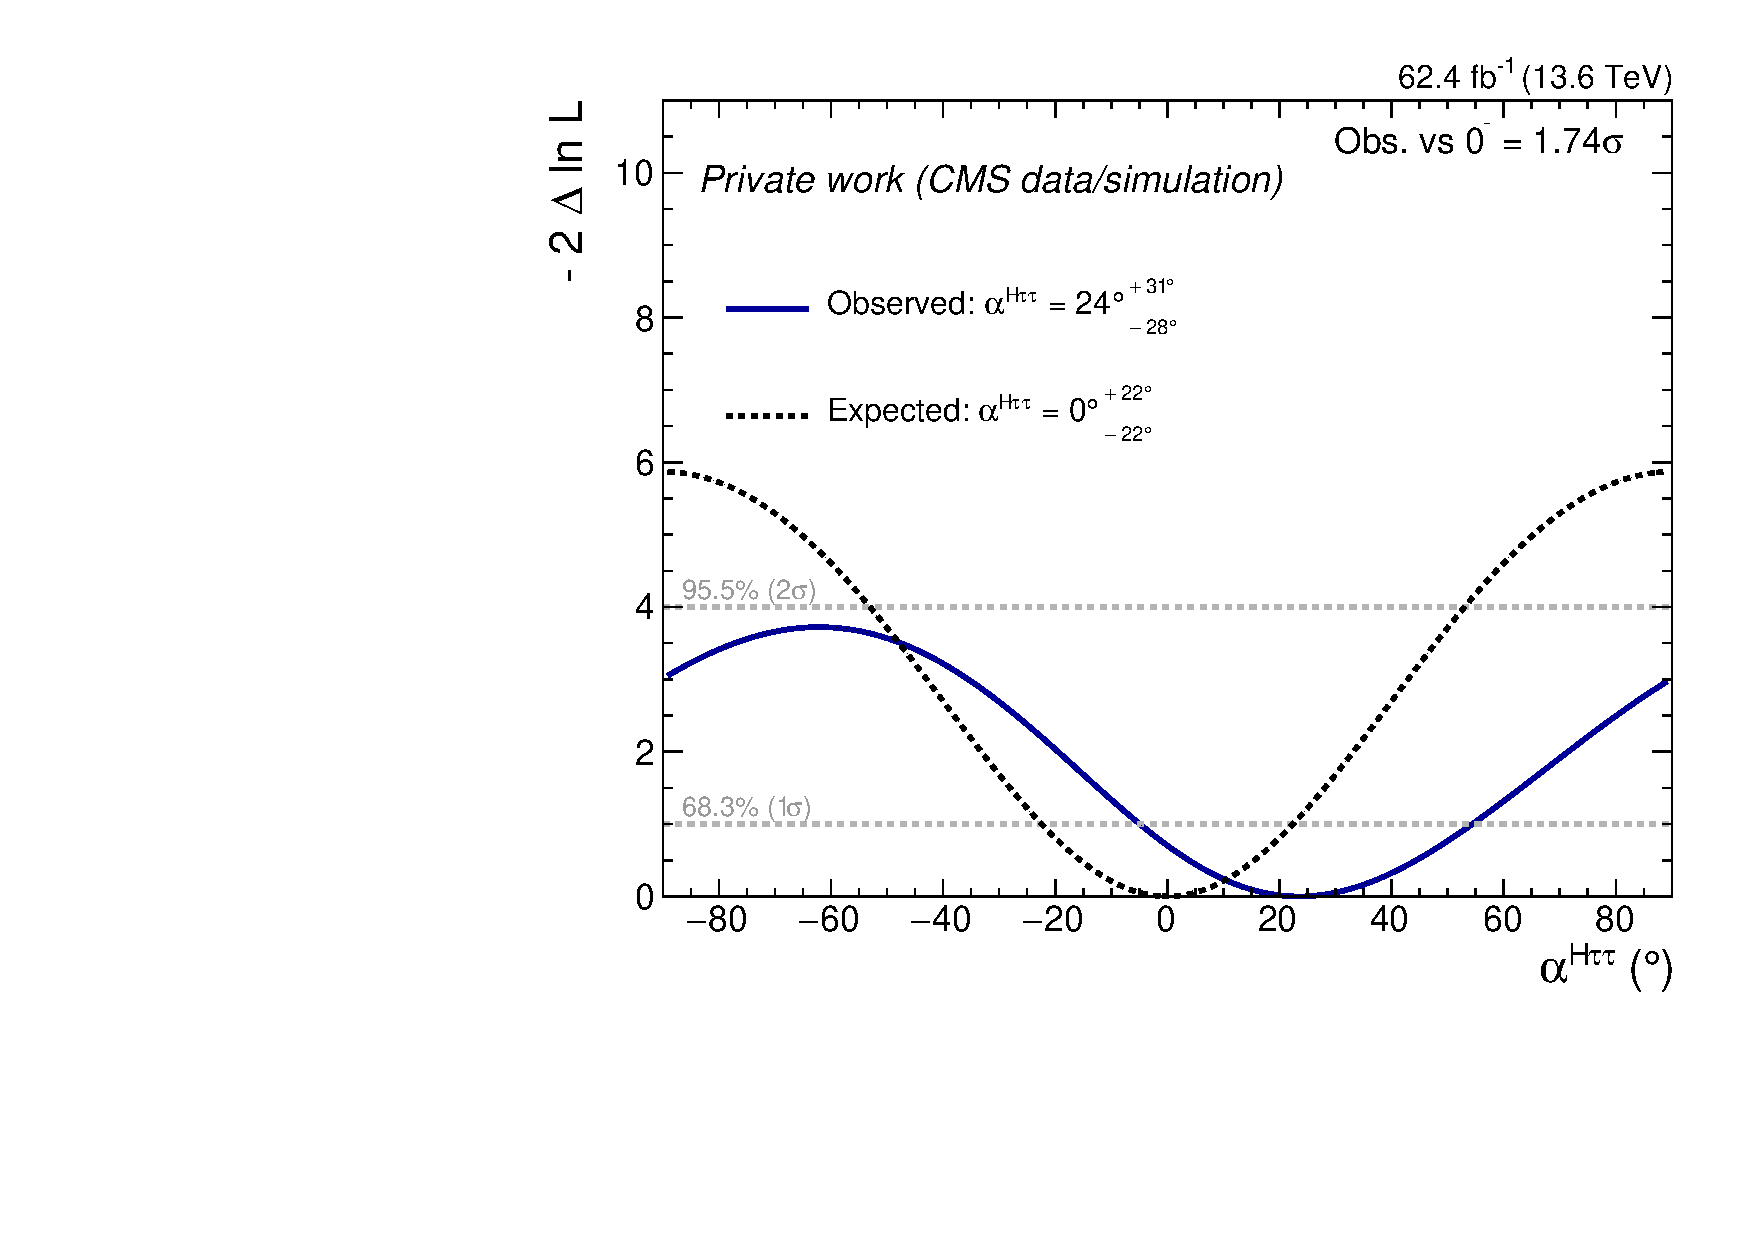
\includegraphics[width=0.9\textwidth]{Figures/Chapter7/alpha/alpha_Run3.pdf}
    \caption{Negative log-likelihood scan of the mixing angle $\alpha^{\PH\tau\tau}$ in the Run 3 analysis.}
    \label{Figure:Chapter7_LLScan}
\end{figure}

The present result ($\alpha^{\PH\tau\tau} = 24 ^{+31^{\circ}}_{-28^{\circ}}$) is consistent with previous measurements of the same parameter. The CMS analysis using the full Run 2 dataset reported $\alpha^{\PH\tau\tau} = -1 \pm 19^{\circ}$ (observed) and $0 \pm 21^{\circ}$ (expected) at the 68.3\% CL~\cite{HiggsCP_CMS_2021}, as discussed earlier in this chapter. The ATLAS collaboration obtained $\alpha^{\PH\tau\tau} = 9 \pm 16^{\circ}$ (observed) and $0 \pm 28^{\circ}$ (expected)~\cite{ATLAS:2022akr}, with their observed sensitivity also affected by statistical fluctuations, in that case leading to stronger observed limits than expected. This measurement is in agreement with both results, and remains compatible with the \ac{SM} expectation of $\alpha^{\PH\tau\tau} = 0^{\circ}$ within uncertainties. In a similar fashion to the previous measurements, the sensitivity of this analysis is predominantly limited by the statistical uncertainty of about $24^{\circ}$, while the contributions from bin-by-bin uncertainties, theoretical modelling, and experimental systematics are subdominant.

\subsection{Sensitivity comparison with the CMS Run 2 analysis}

This measurement has introduced several methodological improvements compared to its Run 2 precursor~\cite{HiggsCP_CMS_2021}, including advances in tau identification, refined event categorisation, and an optimised reconstruction of the CP-sensitive observable (see Section~\ref{Section:Chapter7_Introduction}). Since inherently the measurement is dominated by statistical uncertainties, it has been a challenge to approach or even surpass the sensitivity of the full Run 2 study while working with a dataset that has less than half the statistical power. To enable a meaningful comparison, the expected sensitivity is evaluated separately for each event category. The results are summarised in Table~\ref{Table:Chapter7_Run2Run3_PerCat_Comp}. 

\begin{table}[!htbp]
\centering
\renewcommand{\arraystretch}{1.5} % Increase row height
\setlength{\tabcolsep}{10pt} % Increase column width
\arrayrulecolor{black} % Ensure outer border is black
\begin{tabular}{ccc}
\hline
\multirow{2}{*}{Category} & \multicolumn{2}{c}{Expected sensitivity [$\sigma$]} \\
         & Run 2 ($137~\mathrm{fb}^{-1}$)  & Run 3 ($62.4~\mathrm{fb}^{-1}$) \\
\hline
$\rho\rho$       & 1.10 & 1.36 \\
\arrayrulecolor{lightgray} \hline
$\rho \pi$       & 1.08 & 1.21 \\
\arrayrulecolor{lightgray} \hline
$\rho a_1^\text{3pr}$       & 0.65 & 1.12 \\
\arrayrulecolor{lightgray} \hline
$\pi\pi$       & 0.39 &  0.41 \\
\arrayrulecolor{lightgray} \hline
$\pi a_1^\text{3pr}$  & 0.48 & 0.70 \\
\arrayrulecolor{lightgray} \hline
$a_1^\text{1pr}\rho + a_1^\text{1pr}a_1^\text{1pr}$  & 0.30 & 0.49 \\
\arrayrulecolor{lightgray} \hline
$\pi a_1^\text{1pr}$       & 0.23 & 0.29 \\
\arrayrulecolor{lightgray} \hline
$a_1^\text{3pr} a_1^\text{3pr}$       & 0.28 & 0.41 \\
\arrayrulecolor{lightgray} \hline
$a_1^\text{3pr} a_1^\text{1pr}$       & 0.13 & 0.27 \\
\arrayrulecolor{black} \hline
\end{tabular}
\caption[Comparison of per-category sensitivities in Run 2 with reconstruction strategies in Run 3.]
{Summary of the expected sensitivity per category in the Run 2 analysis~\cite{HiggsCP_CMS_2021} (second column), compared with the reconstruction strategy adopted for the present Run 3 analysis (third column).}
\label{Table:Chapter7_Run2Run3_PerCat_Comp}
\end{table}

An improvement in sensitivity is observed across all categories relative to the Run 2 analysis. The largest gain is achieved in categories involving one $a_1^{3\mathrm{pr}}$ decay, where the $\phi_{CP}$ reconstruction method has been substantially overhauled (see Section~\ref{Section:Chapter7_CombinedMethods}). Overall, the expected exclusion of the pure CP-odd scenario in the $\PH\to\tau_h\tau_h$ alone reaches $2.39\sigma$, compared to $1.85\sigma$ in Run 2~\cite{HiggsCP_CMS_2021}, despite the reduced statistical power of the datasets used in this analysis. This improvement underscores the effectiveness of the methodological refinements introduced in Run 3 and illustrates the potential impact they could deliver, both in future analyses with larger Run 3 datasets and in a possible re-analysis of the full Run 2 data.

\subsection{Combination with the CMS Run 2 result}

A statistical combination of this measurement with the previous CMS Run 2 result has been performed to maximise sensitivity to the CP structure of the $\PH\tau\tau$ Yukawa coupling. Since both analyses are dominated by statistical uncertainties, only a subset of systematic effects is treated as correlated between the two. Theoretical uncertainties on production cross sections and branching ratios are considered correlated, with the exception of backgrounds, where different generators are used across the two analyses. Similarly, top-quark $p_\text{T}$ reweighting uncertainties are treated as correlated, whereas uncertainties from Z $p_\text{T}$-mass reweighting are decorrelated due to the different modelling strategies employed in the two analyses.

For theory uncertainties affecting the signal acceptance and shape, a conservative approach is adopted. For the \ac{ggH} process, different event generators are used in Run 2 and Run 3, and the associated uncertainties are therefore decorrelated. For \ac{VBF}, uncertainties from parton-shower modelling are correlated, but QCD scale variations are not, since their implementation differs between the two analyses. Experimental uncertainties are mostly decorrelated, reflecting the distinct reconstruction strategies and treatments applied in the two data-taking periods. Overall, the combination remains statistics-limited, and the exact treatment of subdominant systematic sources has only a minor impact on the final result.

Following the strategy of the individual analyses, the combination is performed with a single rate parameter left free to float in the fit, scaling the overall signal strength. The resulting negative log-likelihood scan is shown in Fig.~\ref{Figure:Chapter7_Combined_LLScan}. The pure CP-odd hypothesis is disfavoured at a significance of $3.55\sigma$, and the extracted mixing angle is measured with an uncertainty of $\pm 15^\circ$ at the 68.3\% CL. This represents the most precise determination of $\alpha^{\PH\tau\tau}$ to date, improving upon both the standalone Run 2 and Run 3 results.

\begin{figure}[!htbp]
    \centering
    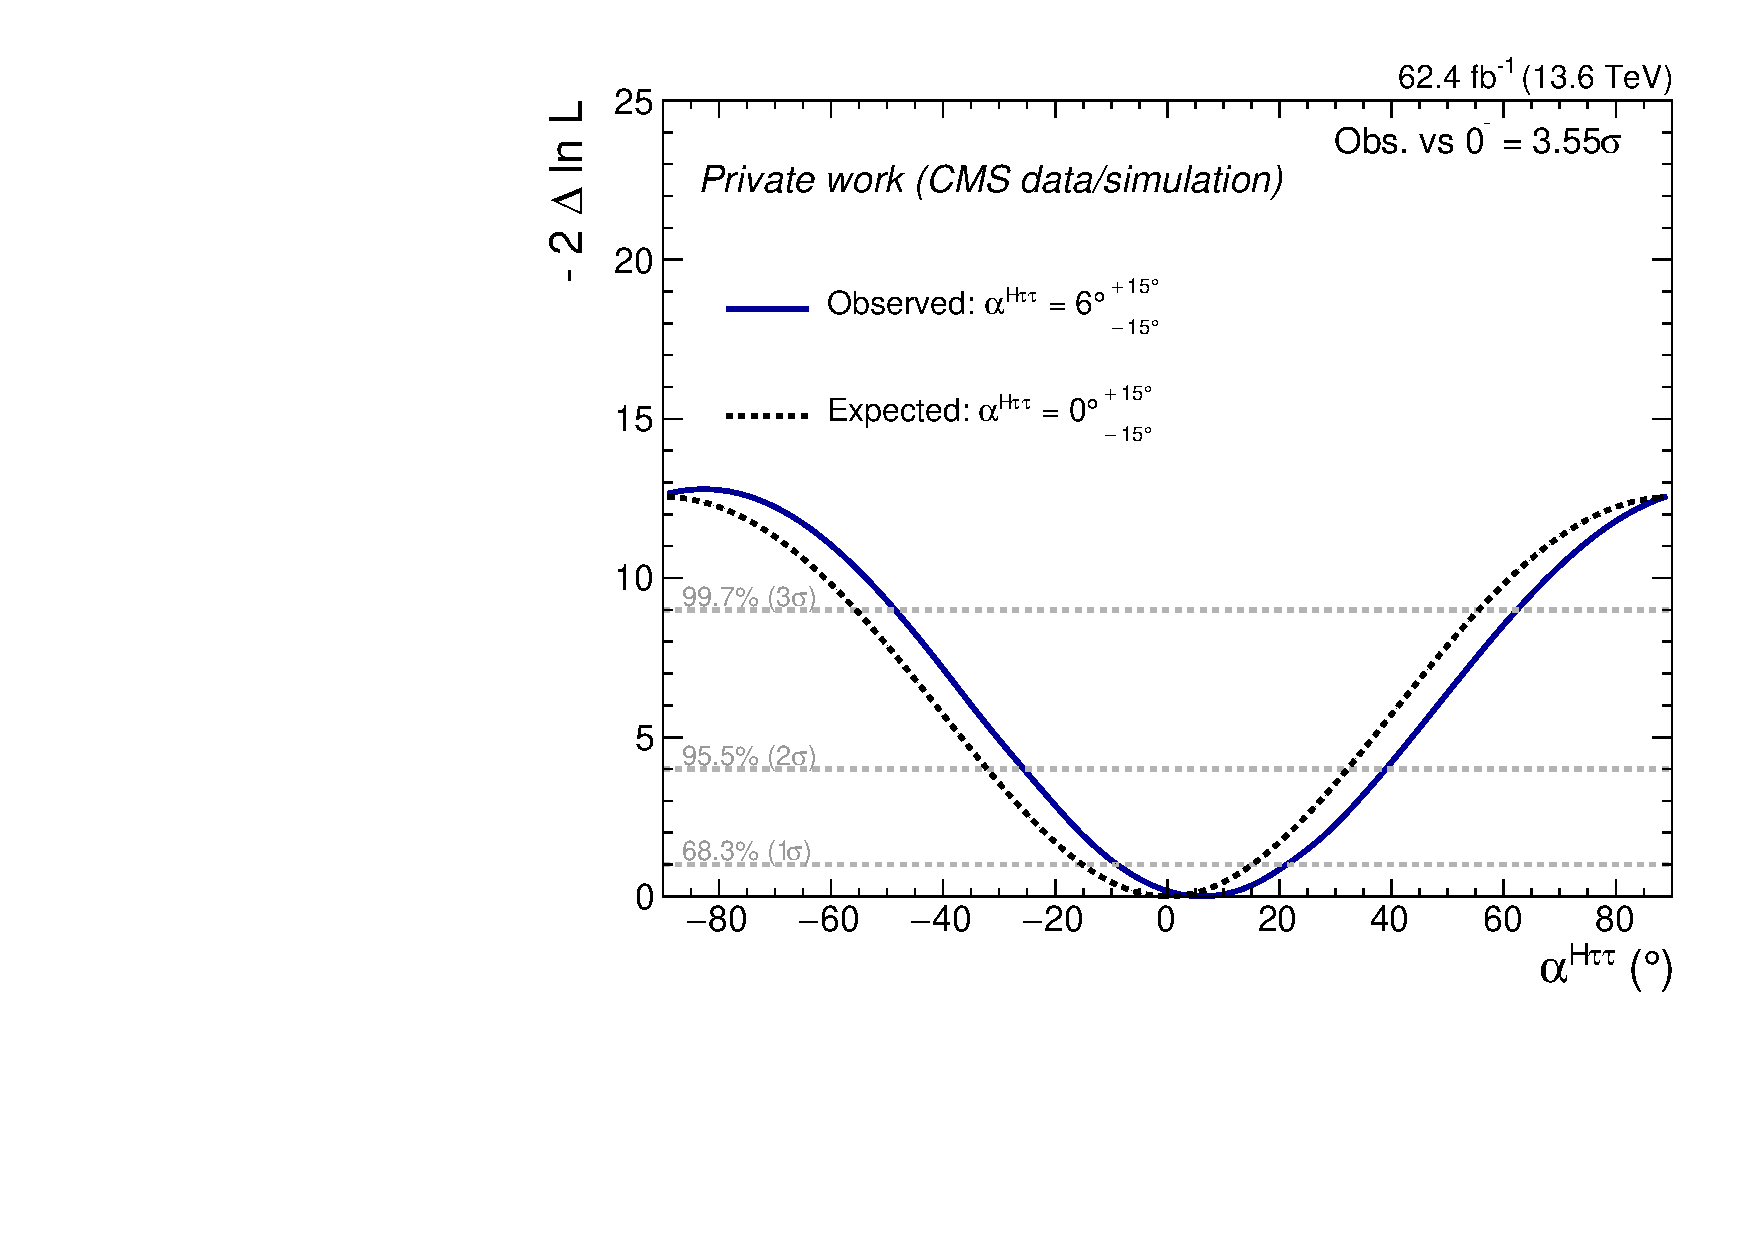
\includegraphics[width=0.9\textwidth]{Figures/Chapter7/alpha/alpha_Run2_3.pdf}
    \caption{Negative log-likelihood scan of the mixing angle $\alpha^{\PH\tau\tau}$ from the combined Run 2 and Run 3 analyses.}
    \label{Figure:Chapter7_Combined_LLScan}
\end{figure}